\documentclass[11pt]{book}

\usepackage{amssymb}
\usepackage{amsmath}
\usepackage{upquote}
\usepackage[]{listings}
%\usepackage{apacite}
\usepackage[font=small,labelfont=bf,indention=0.5cm,aboveskip=20pt]{caption}
\usepackage[amsmath,thmmarks,standard]{ntheorem}
\usepackage{etex}
\usepackage{ifthen} 
\usepackage{graphicx}
\usepackage[]{subfig}
\usepackage[margin=0.75in]{geometry}
\usepackage{makeidx}
%\usepackage{layout} % this allows to print the layout data of the actual class
\usepackage[authoryear,round]{natbib}
\usepackage[avoideditors,withbib,pages]{authorindex} 
%\usepackage[T1]{fontenc}
\usepackage[final]{animate}
\usepackage{tabularx}
\usepackage[colorlinks]{hyperref}
\usepackage{cleveref}
\usepackage{mymath}
\usepackage{ocmat}
\makeindex
%\bibliographystyle{plain}
%\bibliographystyle{apacite}

% defined for the subfigure command
\newcommand{\goodgap}{%
\hspace{\subfigtopskip}%
\hspace{\subfigbottomskip}}

%\lstset{breaklines=true,language=Matlab,basicstyle=\small,escapeinside={(*@}{@*)}}
\lstset{breaklines=true,basicstyle=\ttfamily,escapeinside={(*@}{@*)}}
\begin{document}
\bibliographystyle{newapa}
%\layout
\frontmatter
\begin{titlepage}
\title{\OCT\ v0.1 Manual}
\author{Dieter Grass\thanks{dieter.grass@tuwien.ac.at} \and Andrea Seidl\thanks{andrea.seidl@tuwien.ac.at}}
\date{}
\maketitle
\end{titlepage}

\newpage
\tableofcontents
\preface{}
\addcontentsline{toc}{chapter}{Preface}

\part{Standard Optimal Control Model}
\label{part:user_man}
\chapter{Introduction}
%\section{Introduction}

The \OCT\ toolbox is a collection of functions designed to adequately handle optimal control problems in \MATL\TReg\footnote{\MATL\ is a registered trademark of The MathWorks Inc.}. The primary focus of this toolbox lies on discounted, autonomous infinite time horizon models, but it also provides extensions to (non-autonomous) finite time horizon problems. Relying on Pontryagin's \MAXP, at its core is the formulation and solution of boundary value problems in combination with a continuation algorithm. This approach allows a systematic numerical analysis of the problem under varying conditions, like changing initial states or parameter values and therefore the detection of bifurcations of the optimal system. It was \emph{not} the intention to provide a general solver for a wide variety of \OCPRO s, or a very fast solver. The typical situation for the usage of \OCMAT\ is a rather low-dimensional problem in the state space (even though there is no principle limit on the number of states or controls) and analytical functional terms describing the dynamics, objective function and constraints.  

A further advantage of \OCMAT\ is the possibility to derive the first order necessary optimality conditions automatically using the symbolic toolbox of \MATL. This frees the user from this often tedious and error-prone step. Additionally the user also has the possibility to provide the optimality conditions by her/his own, which becomes important if a specific situation has to be considered, that is not included in the standard case. Furthermore, the necessary \MATL\ files are generated automatically, which speeds up the time between model formulation and start of the numerical analysis considerably. 

This automatization process for the file generation relies on the provision of so called template files. These files are pure ASCII files (extension 'oct') and contain variables, which are then replaced by the model specific values. A simple script language also allows the usage of ``if-else'' clauses and ``for'' loops supporting the adaptation on specific needs. An experienced user should therefore be able to write her/his own template files and extending the capabilities of \OCMAT.

Another intention for the development of \OCMAT\ was to create a tool that researchers with only little (mathematical) background knowledge can use for the analysis of standard optimal control models. However, some basic knowledge about the underlying ideas and methods is certainly helpful and for non-standard models even necessary. Introductory books to optimal control theory are numerous, one of these is \cite{grassetal2008} which was written simultaneously to the development of the toolbox. All of the numerical results presented in this book were calculated with \OCMAT. For a first introduction to the used numerical methods the user is referred to \citet{grass2012}. 

But not only problems of mathematical nature were a concern for the design of this toolbox. As a large quantity of information has to be handled, another objective of the toolbox is to ensure that users can efficiently access information interesting not only from a mathematician's point of view, but also information relevant for the economic interpretation of the analyzed model. Closely related is the goal that as much as possible can be handled automatically without losing information, as well as providing ways to influence the outcome. It was also important not to neglect the possibility of further extensions of the toolbox. For all these reason an objective oriented programming approach was used for \OCMAT.

The aim of this manual is to present the main features of the \OCMAT\ toolbox and to provide some guidance to users about how to use it. Additional information are included in the files of the specific functions. Further, on the website\footnote{\httpOCMAT} some demos are provided in order to illustrate \OCMAT's main capabilities.

\section{First Steps for Installation}
\subsection*{System Requirements}
\OCMAT\ requires the correct installation of \MATL\ V.7 or higher. At the moment the derivation of the necessary optimality conditions only work for the Symbolic Toolbox relying on the Maple kernel (\MATL\ V.7.5 and lower). \OCMAT\ accesses by default also the Optimization Toolbox, but this is not a necessary requirement.

For bifurcation related calculations it is suggested that the package \CLMATCONT\ \footnote{download from \httpMATCONT.} is installed on a path accessible to \MATL.

\subsection*{General Preparation}
In order to run \OCMAT, take the following steps:
\begin{enumerate}
\item Make sure you have correctly installed \MATL\ and the necessary toolboxes.
\item Download the \OCMAT-Toolbox and unzip it into any directory where \MATL\ can find it (or add the directory to the \MATL\ path).
\item You can have different versions of \OCMAT\ at the same time, only make sure that \MATL\ has the ``right'' version on its path.
\end{enumerate}

\section{Model Class}
To help the novice in becoming acquainted with the optimal control toolbox (\OCMAT) we start with a simple class of problems. This has the advantage that we can concentrate on the basic concepts without getting lost in technicalities. Thus, we consider 
\begin{subequations}
\label{eq:simple_simple_opt_pro}
\begin{align}
& \max_{u(\cdot)}\int_0^\infty\E^{-rt}g\left(x(t),u(t),\modelpar\right)\,\Dt\label{eq:simple_opt_pro_obj}\\
\text{s.t.}\quad & \dot{x}(t) =\f\left(x(t),u(t),\modelpar\right),\quad t\in[0,\,\infty)\label{eq:simple_opt_pro_dyn}\\
& \mixc\left(x(t),u(t),\modelpar\right)\ge0,\quad t\in[0,\,\infty)\label{eq:simple_opt_pro_mc}\\
\text{with}\quad & x(0) = x_0\label{eq:simple_opt_pro_init}
\end{align}
\end{subequations}
where the state dynamics $f\colon\R^{n+m}\rightarrow\R^n$, the objective function $g\colon\R^{n+m}\rightarrow\R$ and the constraint $\mixc\colon\R^{n+m}\to\R^k$ are assumed to be as often continuously differentiable in their arguments as necessary. Moreover the model is assumed to be nonlinear in the control variable $u\in\R^m$.


\mainmatter 
\chapter{Basic Model}
\label{sec:standardmodel}
For a concrete model we use the so called ``model of moderation'' (\MoM) which is analyzed in \citet{caulkinsetal2005a} and given by
\begin{subequations}
\label{eq:mom}
\begin{align}
& \max_{u(\cdot)}\int_0^\infty\E^{-rt}\left(x(t)^2+cu(t)^2\right)\,\Dt\label{eq:mom1}\\
\text{s.t.}\quad & \dot{x}(t)=x(t)\left(1-x(t)^2\right)+u(t),\quad t\ge0\label{mom2}\\
\text{with}\quad & x(0) = x_0.\label{eq:mom3}
\end{align}
\end{subequations}
Model \cref{eq:mom} consists of one state $x$ and one control $u$ and is obviously member of the class of models \cref{eq:simple_simple_opt_pro}. 

\section{Initialization}
\label{sec:InitializationMoM}
In the subsequent sections the initialization process for \MoM\ is presented. The following steps are necessary and will subsequently be carried out in detail.
\begin{enumerate}
	\item Preparation of an initialization file (plain ASCII file).
	\item Process the initialization file to generate the necessary optimality conditions. (We assume that the symbolic toolbox is installed.)
	\item Start auto-generation of the model files.
\end{enumerate}

\subsection{Initialization File}
\label{sec:InitializationFile}
Initialization files are plain ASCII files with extension (\lstinline+.ocm+) and a specific syntax, that allows \OCMAT\ to identify the model structure and therefore derive the necessary optimality conditions. The following example for \MoM\ is a minimal example, since only mandatory parts are included. We generate a file \lstinline+mom.ocm+ consisting of
\begin{ocmlisting}
Variable
state::x
control::u

Statedynamics
ode::Dx=x-x^3+u

Objective
int::-(x^2+c*u^2)

Parameter
r::1
c::1
\end{ocmlisting}
The empty lines between the different sections can be omitted and are only kept for better readability. There are four mandatory sections that have to appear in each initialization file. The signal words \lstinline+Variable+, \lstinline+Statedynamics+, \lstinline+Objective+ and \lstinline+Parameter+ are case insensitive but have to appear in a separate line. Comments starting with \lstinline+%+ are allowed at any place.

\paragraph{Variable}
\label{sec:Variable}
The lines following the signal word \lstinline+Variable+ define the variable names for the state and the control variable(s). The syntax is 
\begin{ocmlisting}
variable::variablename
\end{ocmlisting}
where \lstinline+variable+ can be one of the following types
\begin{itemize}
	\item state
	\item control
	\item costate (default variable name \lstinline+lambda1,lambda2,+ etc.).
\end{itemize}
The \lstinline+variablename+ has to be a name satisfying the \MATL\ rules for variable names. If there exist more than one \lstinline+variable+ the variable names have to be comma separated
\begin{ocmlisting}
variable::variablename1,variablename2
\end{ocmlisting}
or according to \MATL\ convention
\begin{ocmlisting}
variable::variablename1:variablename4
\end{ocmlisting}
which is a short cut for
\begin{ocmlisting}
variable::variablename1,variablename2,variablename3,variablename4
\end{ocmlisting}
The main reason for specifying the variable names explicitly is for a better readability for the user, who is familiar with her/his own denomination and need not adapt to a standard notation.\footnote{In the auto-generated model files such a standard notation is used, where, e.g. state and costates are replaced by the variable name \lstinline+depvar+ (for dependent variables) with an index. Symbolic expressions of terms, like the Hamiltonian, are returned (using, e.g., the command \lstinline+hamiltonian(m)+) in the user denomination.}

\paragraph{Statedynamics}
\label{sec:Statedynamics}
The syntax for the state dynamics is as follows
\begin{ocmlisting}
ode::Dx=f(x,u)
\end{ocmlisting}
where \lstinline+f(x,u)+ is some algebraic term for the differential equation.
Each state dynamics has to be written in an extra line.

%For a two state model with state variables $F$ and $A$ this becomes
%\begin{ocmlisting}
%Statedynamics
%ode::DF=sigma*F*(1-F/(m*A))-gamma/(C+tau)*(F^theta1/(1+F^theta2))-eta*h*F
%ode::DA=(n-d*A-e*A*F)/epsilon
%\end{ocmlisting}

\paragraph{Objective}
\label{sec:Objective}
The objective section lets you specify the actual function that has to be optimized. Usually this will be a (discounted) integral, and the syntax is
\begin{ocmlisting}
int::g(x,u)
\end{ocmlisting}
where \lstinline+g(x,u)+ is some algebraic expression for the integrand of the following integral
\begin{equation*}
	\int\E^{-rt}g(x(t),u(t))\,\Dt.
\end{equation*}
Without additional information it is assumed that the integrand is exponentially discounted and the variable for the discount rate is $r$ by default. To use a different variable name for the discount rate, e.g. \lstinline+rho+, you can additionally specify
\begin{ocmlisting}
expdisc::rho
int::g(x,u)
\end{ocmlisting}
Also note that by default the problem is considered as a maximization problem and therefore the objective function for \MoM\ as it is given in \cref{eq:mom1} is multiplied by minus one in the initialization file. %Subsequently we will show how to change the optimization type to minimization.

\paragraph{Parameter}
\label{sec:Parameter}
For each of the parameter variables that appear in the functional forms of the model a value has to be provided in the form
\begin{ocmlisting}
r::1
c::1
\end{ocmlisting}
It is also allows to provide functional expressions like
\begin{ocmlisting}
r::exp(0)+6
c::sqrt(2)
\end{ocmlisting}

\subsection{Processing the Initialization File}
\label{sec:ProcessingInitializationFile}
Next the necessary optimality conditions and further information about the model have to be processed within \OCMAT. During this step the default model folders, where files and data are stored, will be generated. These folders are
\begin{pathlisting}
ocmat\model\usermodel\[modelname]
ocmat\model\usermodel\[modelname]\data
\end{pathlisting}
Moreover, a structure \lstinline+ocStruct+ will be generated, containing the model specific properties. This structure is stored in
\begin{pathlisting}
ocmat\model\usermodel\[modelname]\data\[modelname]ModelDataStructure.mat
\end{pathlisting}
For the model \MoM\ the process is initiated by
\begin{matlab}
>> ocStruct=processinitfile('mom');(*@\index{Command!Initialization!\lstinline+processinitfile+}@*)
.\ocmat\model\usermodel\mom does not exist. Create it?  y/(n): y
.\ocmat\model\usermodel\mom\data does not exist. Create it?  y/(n): y
.\ocmat\model\usermodel\mom\data is not on MATLAB path. Add it?  (y)/n: y
\end{matlab}
The main fields of the structure \lstinline+ocStruct+ are
\begin{matlab}
ocStruct = 

             modeltype: 'standardmodel'
             modelname: 'mom'
              variable: [1x1 struct]
            constraint: [1x1 struct]
             objective: [1x1 struct]
             parameter: [1x1 struct]
                   arc: [1x1 struct]
    pontryaginfunction: [1x1 struct]
                   foc: [1x1 struct]
\end{matlab}
E.g., the field \lstinline+foc+ itself is a structure containing the first order necessary optimality conditions. %For a detailed description of the structure see \cref{sec:ocStruct}.

\subsection{Generating the Model Files}
\label{sec:GeneratingTheModelFiles}
In the last step the necessary model files are generated and moved to the default model folder. To start the file generation call the command
\begin{matlab}
>> modelfiles=makefile4ocmat(ocStruct);(*@\index{Command!Initialization!\lstinline+makefile4ocmat+}@*)
\end{matlab}
The variable \lstinline+modelfiles+ is a structure consisting of the file names and some properties that were generated, e.g.
\begin{matlab}
>> strvcat(modelfiles.name)

ans =

ArcInfo                           
ArcDiscretizationInfo             
CanonicalSystem                   
EquilibriumEquation               
SymbolicCanonicalSystem           
CanonicalSystemJacobian           
CanonicalSystemParameterJacobian  
CanonicalSystemHessian            
CanonicalSystemTotalHessian       
OptimalControl                    
SymbolicOptimalControl            
LagrangeMultiplier                
SymbolicLagrangeMultiplier        
Hamiltonian                       
DHamiltonianDx                    
D2HamiltonianDu2                  
SymbolicHamiltonian               
4SaddlePathContinuation           
4IndifferenceSolutionContinuation 
BCJacobian4Initial                
BCJacobian4Asymptotic             
BCJacobian4Guard                  
BCJacobian4Reset                  
Admissible                        
UserAdmissible                    
UserFunction                      
ObjectiveFunction                 
ObjectiveFunctionJacobian         
ObjectiveFunctionParameterJacobian
Constraint                        
PlotIndifferenceContinuation      
PlotContinuation          
\end{matlab}
For each of these files a corresponding template file has to exist. These template files are plain ASCII files and provide the structure, that is filled by the specific functional forms of a model. Calling the command \lstinline+makefile4ocmat+ generates these files and store the files in the intermediate folder
\begin{pathlisting}
\ocmat\model\usermodel\out
\end{pathlisting}
This step is mainly interposed for security reasons that the user may check the files and decide if s/he wants to replace maybe older model files from a previous model installation. 

To move the files to the actual model folder, e.g.
\begin{pathlisting}
\ocmat\model\usermodel\mom
\end{pathlisting}
call the \MATL\ command
\begin{matlab}
>> moveocmatfiles(ocStruct,modelfiles)(*@\index{Command!Initialization!\lstinline+moveocmatfiles+}@*)
\end{matlab}
If the model files already exist you are asked if you want to overwrite the older files by the actual files.

\subsection{Model Instance}
\label{sec:modelinstance}
The default instance of the standard optimal control model \lstinline+stdocmodel+\index{Command!\lstinline+stdocmodel+} \MoM\ is initiated by
\begin{matlab}
>> m=stdocmodel('mom')
Model data structure successfully loaded from data file:
.\ocmat\model\usermodel\mom\data\momModelDataStructure.mat
m =
ocmatclass: stdocmodel
    modelname : mom
    r : 1
    c : 2
\end{matlab}
This loads the data structure for model \MoM\ and assigns the corresponding \MATL\ class \lstinline+stdocmodel+ for model \cref{eq:mom} to \lstinline+m+. The parameter values are the default values specified in the initialization file.

This class consists of the two fields \lstinline+Model+ (mainly the data structure) and \lstinline+Result+, where the latter is empty for a new instance. All results of an analysis will then be written into this field and the specific instance can be saved
\begin{matlab}
>> save(m)
\end{matlab}
This stores the actual instance \lstinline+m+ into a \lstinline+mat+-file with default name \lstinline+mom_r_1_c_2.mat+ (composed of the model name and its parameter values) at the default model data folder \lstinline+.\ocmat\model\usermodel\mom\data+.

To generate an instance with different parameter values, these can be changed using
\begin{matlab}
>> m=changeparametervalue(m,'r',0.1);\index{Command!stdocmodel!changeparametervalue}
\end{matlab}
or to change more than one parameter value at once
\begin{matlab}
>> m=changeparametervalue(m,'r,c',[0.1 2]);
\end{matlab}

\subsection{Retrieving Model Information}
There exists a large number of commands that allow the user either to evaluate expressions, e.g. canonical system, Hamiltonian, etc., at specific points or to return the corresponding symbolic expressions. In the following a few of these commands are presented.

With \lstinline+control+ the symbolic expression for the control value is returned
\begin{matlab} 
>> u=control(m)
u =
-1/2*lambda1/c
\end{matlab}
Similar the expression of the Hamiltonian is returned by
\begin{matlab} 
>> H=hamiltonian(m)
H =
x^2+c*u^2+lambda1*(x-x^3+u)
\end{matlab}
We note that the control variable \lstinline+u+ is not replaced by its optimal expression. To get the maximized Hamiltonian, i.e., where the control variable is substituted by the corresponding expression from the Hamiltonian maximizing condition, the following command can be used
\begin{matlab} 
>> H_opt=hamiltonian(m,[],[],1)
H_opt =
x^2+1/4/c*lambda1^2+lambda1*(x-x^3-1/2*lambda1/c)
\end{matlab}
The empty arguments are necessary and will be explained in due course. Analogous to the latter case we find the canonical system by
\begin{matlab} 
>> dxdt=canonicalsystem(m)
dxdt =
                           x-x^3+u
 r*lambda1-(2*x+lambda1*(1-3*x^2))
\end{matlab}
or with replaced control variable
\begin{matlab} 
>> dxdt_opt=canonicalsystem(m,[],[],1)
dxdt_opt =
             x-x^3-1/2*lambda1/c
 r*lambda1-2*x-lambda1*(1-3*x^2)
\end{matlab}
To find the expressions where the parameter variables are replaced by the values of the actual instance \lstinline+m+ we can, e.g., call
\begin{matlab} 
>> H_rep=subsparametervalue(m,H_opt)
H_rep =
x^2+1/8*lambda1^2+lambda1*(x-x^3-1/4*lambda1)
\end{matlab}

\section{Numerical Analysis}
\label{sec:numanalysis}
After a successful initialization of the model the numerical analysis can immediately start. Subsequently we present the basic steps of an analysis. This includes the determination of equilibria of the canonical system and the calculation of stable paths. Since equilibria and trajectories are central objects of the analysis these are implemented as \MATL-classes (see \cref{sec:classdesign}).

\subsection{Equilibria}
\label{sec:numanalysis_equilib}
In its simplest form the equilibria can be found by
\begin{matlab} 
>> ocEP=calcep(m)(*@\index{Command!dynprimitive!\lstinline+calcep+}@*)
ocEP = 
    [1x1 dynprimitive]
    [1x1 dynprimitive]
    [1x1 dynprimitive]
    [1x1 dynprimitive]
    [1x1 dynprimitive]
\end{matlab}
For our example and the actual parameter values of the instance \lstinline+m+ five equilibria, each of them is represented by a member of the class \lstinline+dynprimitive+, are detected. The returning argument assigned to \lstinline+ocEP+ is a cell array of \lstinline+dynprimitive+ objects.

To find the equilibria by \lstinline+calcep(m)+ it is assumed that the symbolic expressions of the canonical system
\begin{matlab} 
>> dxdt_rep=subsparametervalue(m,dxdt_opt)(*@\index{Command!stdocmodel!\lstinline+subsparametervalue+}@*)
dxdt_rep =
             x-x^3-1/4*lambda1
 lambda1-2*x-lambda1*(1-3*x^2)
\end{matlab}
can be solved by the symbolic toolbox of \MATL.\footnote{I.e. the equations are solved using the \MATL\ command \lstinline+solve(dxdt_rep(1),dxdt_rep(2),'x','lambda1')+} Otherwise further arguments have to be provided and a numerical procedure is used, which will be explicated in the next chapter.

The class structure of \lstinline+dynprimitive+ allows an easy manipulation of the objects and access to the basic properties. Basic information about the values and the eigenvalues of an equilibrium, e.g., for the second equilibrium of the previous example, are displayed in the workspace simply writing
\begin{matlab} 
>> ocEP{2}
ans =
ocmatclass: dynprimitive
modelname: mom
Equilibrium:
   -0.8881
   -0.7507
Eigenvalues:
   -1.2269
    2.2269
Arcidentifier:
     0
\end{matlab}
For the subsequent examples let us assign the second equilibrium to the variable \lstinline+dynPrim+, i.e.
\begin{matlab} 
>> dynPrim=ocEP{2};
\end{matlab}
To retrieve the values of \lstinline+dynPrim+ the following commands can used
\begin{matlab} 
>> y=dynPrim.y;
\end{matlab}
or equivalently
\begin{matlab} 
>> y=dependentvar(dynPrim);(*@\index{Command!dynprimitive!\lstinline+dependentvar+}@*)
\end{matlab}
For the Jacobian write
\begin{matlab} 
>> J=dynPrim.linearization;
\end{matlab}
or equivalently
\begin{matlab} 
>> J=jacobian(dynPrim);(*@\index{Command!dynprimitive!\lstinline+jacobian+}@*)
\end{matlab}
Due to the importance of eigenvectors and eigenvalues for the calculation of solution paths the \MATL\ command \lstinline+eig+ was overloaded for the \lstinline+dynprimitive+ class. Thus,
\begin{matlab} 
>> [vec val]=eig(dynPrim);(*@\index{Command!dynprimitive!\lstinline+eig+}@*)
\end{matlab}
returns the eigenvectors and eigenvalues.

Members of the class \lstinline+dynprimitive+ can be used as (second) arguments for the commands like, \lstinline+hamiltonian+, \lstinline+control+, \lstinline+canonicalsystem+, etc. Then the particular expressions are evaluated at the specific equilibrium, e.g.
\begin{matlab} 
>> H=hamiltonian(m,dynPrim);(*@\index{Command!dynprimitive!\lstinline+hamiltonian+}@*)
>> u=control(m,dynPrim);(*@\index{Command!dynprimitive!\lstinline+control+}@*)
>> dxdt=canonicalsystem(m,dynPrim);(*@\index{Command!dynprimitive!\lstinline+canonicalsystem+}@*)
\end{matlab}
For an equilibrium the last command should return a nullvector, or, due to numerical inaccuracy, a ``near'' nullvector. Additionally the commands
\begin{matlab} 
>> x=state(m,dynPrim);(*@\index{Command!dynprimitive!\lstinline+state+}@*)
>> lambda=costate(m,dynPrim);(*@\index{Command!dynprimitive!\lstinline+costate+}@*)
\end{matlab}
allow to specifically address the state or costate values.

To check if a calculated equilibrium is admissible, i.e. it satisfies the constraints if there are any, the canonical system is zero (or nearly zero) evaluated at the equilibrium and the equilibrium is real valued (or an imaginary part is smaller than some tolerance) the following command can be used
\begin{matlab} 
>> b=isadmissible(dynPrim,m);(*@\index{Command!dynprimitive!\lstinline+isadmissible+}@*)
\end{matlab}
where $b=1$ denotes an admissible equilibrium and $b=0$ an inadmissible equilibrium. It is also possible to check a cell array of \lstinline+dynprimitive+ objects
\begin{matlab} 
>> b=isadmissible(ocEP,m);
\end{matlab}
In that case \lstinline+b+ is a vector of the same size as the cell array with zero and one for (in)admissible equilibria.

To ease the search for saddle points that have to be considered for a further analysis the command \lstinline+issaddle+ can be used
\begin{matlab} 
>> [b dim]=issaddle(dynPrim);(*@\index{Command!dynprimitive!\lstinline+issaddle+}@*)
\end{matlab}
where \lstinline+b+ is one in case of a saddle point and zero otherwise. The argument \lstinline+dim+ denotes the number of eigenvalues with negative real part (dimension of the corresponding stable manifold).

\subsection{Saddle-path}
\label{sec:numanalysis_saddlepath}
The core part of \OCMAT\ is the calculation of a saddle-path corresponding to an equilibrium and starting at some given initial state. The basic numerical concepts are presented in \citet{grass2012}. At this point only the technical steps within the \OCMAT\ environment are explained. To reproduce the process depicted in \cref{fig:uniquemomcont} the following commands have to be called. 
\begin{matlab} 
>> m=changeparametervalue(m,'r',0.5);ocEP=calcep(m);
>> sol=initocmat_AE_EP(m,ocEP{1},1,1.5)(*@\index{Command!continuation!\lstinline+initocmat_AE_EP+}@*)
sol = 
              x: [1x40 double]
              y: [2x40 double]
     parameters: 0
    arcinterval: [0 100]
    timehorizon: Inf
         arcarg: 0
             x0: 0
          idata: [1x1 struct]
>> c=bvpcont('extremal2ep',sol);(*@\index{Command!continuation!\lstinline+bvpcont+}@*)
first solution found
tangent vector to first solution found

 Continuation step No.: 1
 stepwidth: 0.01
 Newton Iterations: 1
 Mesh size: 41
 Continuation parameter: 0.000513129

/* run through continuation steps */

 Continuation step No.: 205
 stepwidth: 0.1
 Newton Iterations: 1
 Mesh size: 93
 Continuation parameter: 1.01721

 Target value hit.
 label=HTV
 Continuation parameter=1
\end{matlab}
First the parameter $r$ is set to $0.05$ and the corresponding equilibria are calculated. Next the continuation process is initialized. The function of the equilibrium \lstinline+ocEP{1}+ is twofold. First it denotes the equilibrium for which the saddle-path is calculated. Second it is used as an initial solution for the underlying \BVP. The third argument denotes the used coordinate for the continuation. The last argument specifies the initial state for the requested solution. The returned argument \lstinline+sol+ is a structure, representing the initial function for the \BVP. 

Finally the continuation process is started, where \lstinline+extremal2ep+ denotes a saddle-path continuation by varying the initial state. The continuation process is depicted graphically (see \cref{fig:uniquemomcont}) and information is displayed in the command window (see the previous listing). The output argument \lstinline+c+ mainly consists of the initial and last detected solution. The information \lstinline+Target value hit.+ (equivalently \lstinline+Continuation parameter=1+) indicates that the solution at the requested initial state $x=1.5$ is reached.

To save the results of the so far carried out calculations, i.e. the equilibria and saddle-path continuation, a storing command is provided.
\begin{matlab} 
>> store(m,ocEP);(*@\index{Command!continuation!\lstinline+store+}@*)
>> store(m,'extremal2ep');
>> save(m)
\end{matlab}
The first two commands store the equilibria and result of the continuation process in the \lstinline+Result+ field of the model \lstinline+m+. The last command saves the entire object (and therefore also the results) as a \lstinline+mat+ file in the default model data folder (see \cref{sec:modelinstance}).
\begin{figure}
\centering
\animategraphics[controls,scale=\scalefactor]{15}{./fig/UniqueMoMContinuation_}{001}{207}
\caption{The graphic display during the continuation process.}
\label{fig:uniquemomcont}
\end{figure}

\subsection{Detection of an Indifference Threshold\index{indifference threshold}}
\label{sec:numanalysis_detindthr}
An interesting phenomenon that consistently appears in \OCPRO, is that of multiple optimal solutions, i.e. initial states for which at least two solutions exist. For a detailed discussion of this phenomenon and the underlying bifurcations the reader is referred to \citet{grassetal2008,kiselevawagener2008a} and \citet{kiseleva2011}. The usual ingredients for the appearance of multiple optimal solutions is the occurrence of multiple equilibria (saddle points). The standard procedure  for the detection of such an indifference threshold (in economic literature also called Skiba point)\index{indifference threshold}\index{Skiba point|see{indifference threshold}} consists of the following steps\footnote{In the presentation we implicitly assume that the model has one state variable. For higher dimensional models the procedure is very similar but needs a more careful explanation.}
\begin{enumerate}
	\item Choose two saddle points $\hat E_{1,2}$.
	\item Calculate the saddle-path starting at the state value of the second equilibrium and converging to the first equilibrium. If an indifference threshold exists such a path does not exist. Usually the saddle-path bends back (limit point) and the continuation process (ideally) stops if the maximum number of continuation steps is reached.\footnote{In case of the existence of an indifference threshold point and if the Hessian matrix of the Hamiltonian with respect to the control variables is strictly convex (maximum), concave (minimium), the saddle-paths cannot be continued to the state values of the other equilibrium, respectively.} Otherwise the user can interrupt the continuation process, pressing the stop button in the ``User Stop'' window.
	\item Repeat the previous step with interchanged roles of the equilibria.
	\item If a region (in the state space) exists, where both saddle paths exist an indifference threshold may exist in this region. To find this point the Hamiltonian is evaluated along both saddle-paths. A possible intersection point denotes the indifference threshold.\footnote{Note that the objective value is given by the Hamiltonian multiplied by the reciprocal of the discount rate $r$ \citep{michel1982}.}
\end{enumerate}
\begin{matlab} 
>> m=stdocmodel('mom');
>> ocEP=calcep(m);store(m,ocEP);
>> opt=setocoptions('OCCONTARG','MaxContinuationSteps',150);
>> sol=initocmat_AE_EP(m,ocEP{1},1,state(m,ocEP{3}));
>> c=bvpcont('extremal2ep',sol,[],opt);
>> store(m,'extremal2ep');
>> sol=initocmat_AE_EP(m,ocEP{3},1,state(m,ocEP{1}));(*@\index{Command!continuation!\lstinline+initocmat_AE_EP+}@*)
>> c=bvpcont('extremal2ep',sol,[],opt);
>> store(m,'extremal2ep');
>> it=findindifferencepoint(m,1,2);(*@\index{Command!stdocmodel!\lstinline+findindifferencepoint+}@*)
\end{matlab}
The last command \lstinline+findindifferencepoint+ computes the indifference threshold by intersecting the Hamiltonian functions corresponding to the two stable paths. The second and third input argument therefore denote the index of the stable path (continuations) as stored in the object \lstinline+m+. Thus, the arguments $1$ and $2$ entail that the indifference threshold is searched by comparing the results of the first and second continuation.

In this approach the value of the indifference threshold depends on the step width of the continuation. To find the (numerical) exact value a \BVP\ can be formulated, that allows the computation of the two optimal paths and therefore the location of the indifference threshold, cf.~\citet{grass2012}.\footnote{A further advantage of this approach is the possible usage of continuation to compute, e.g. an indifference threshold curve in a two state model.} The necessary steps are shown by the following listing of \OCMAT\ commands 
\begin{matlabnum} 
>> sol=initocmat_AE_EP(m,ocEP{1},1,it);(*@\label{li:initocmat_ae_ep_mom}@*)
>> c=bvpcont('extremal2ep',sol,[],opt);
>> store(m,'extremal2ep');
>> sol=initocmat_AE_EP(m,ocEP{3},1,it);
>> c=bvpcont('extremal2ep',sol,[],opt);
>> store(m,'extremal2ep');(*@\label{li:m_store_mom}@*)
>> ocAsym{1}=m.Result.Continuation{3}.ExtremalSolution;(*@\label{li:ocasym1_mom}@*)
>> ocAsym{2}=m.Result.Continuation{4}.ExtremalSolution;(*@\label{li:ocasym2_mom}@*)
>> sol=initocmat_AE_IS(m,ocAsym,1,[]);(*@\label{li:initocmat_ae_is_mom}@*)
>> opt=setocoptions('OCCONTARG','InitStepWidth',0,'MaxContinuationSteps',1);(*@\label{li:setocoptions_mom}@*)
>> c=bvpcont('indifferencesolution',sol,[],opt);(*@\label{li:bvpcont_mom}\index{Command!continuation!\lstinline+bvpcont+}@*)
first solution found
tangent vector to first solution found

 Continuation step No.: 1
 stepwidth: 0
 Newton Iterations: 1
 Mesh size: 127
 Continuation parameter: 0
>> store(m,'indifferencesolution');(*@\label{li:store_mom}@*)
>> save(m)(*@\label{li:save_mom}@*)
Overwrite existing file from 05-Sep-2013 06:14:35 of size 465687 with new size 1891454?  y/(n): y
\end{matlabnum}
To determine an initial function for the indifference threshold \BVP\ the saddle-paths starting at the previously calculated value \lstinline+it+ are computed and stored (\crefrange{li:initocmat_ae_ep_mom}{li:m_store_mom}). These solutions are assigned to a cell array \lstinline+ocAsym+ (\cref{li:ocasym1_mom,li:ocasym2_mom}). Then global variables for the \BVP\ are initialized and the initial function \lstinline+sol+ is returned (\cref{li:initocmat_ae_is_mom}). Next some options are set (\cref{li:setocoptions_mom}). The initial step size is set to zero, because in fact nothing is to be continued. Only the first solution is needed. Therefore also the number of continuation steps is set to one. Finally the computation is started (\cref{li:bvpcont_mom}) and successfully cancels after one step. To keep the result for further processing the solution is stored (\cref{li:store_mom}) and the model is saved (\cref{li:save_mom}).
\begin{figure}
\centering
\animategraphics[controls,scale=\scalefactor]{15}{./fig/MultipleMoMContinuation_}{001}{152}
\caption{The continuation processes for the detection of an indifference threshold.}
\label{fig:multiplemomcont}
\end{figure}
\begin{figure}
\centering
\includegraphics[scale=\scalefactor]{./fig/MultipleMoM}
\label{fig:multiplemom}
\caption{The Hamiltonian evaluated along the saddle-paths intersect in an indifference threshold}
\end{figure}
\begin{remark}
The existence of multiple equilibria in the canonical system does not imply the existence of multiple optimal solutions as the example with $r=0.5$ and $c=2$ shows. In that case the saddle-path of the equilibrium at the origin overlaps the other saddle-points in the state space, cf.~\cref{fig:uniquemomov}
\end{remark}
\begin{figure}
\centering
\includegraphics[scale=\scalefactor]{./fig/UniqueMoMOverlap}
\caption{The saddle-path (right arc) of the equilibrium at the origin (green) overlaps the right saddle-point and its saddle-path (blue)}
\label{fig:uniquemomov}
\end{figure}
\begin{figure}
\centering
\includegraphics[scale=\scalefactor]{./fig/ExactIndifferenceThresholdMoM}
\caption{The (numerical) exact indifference threshold determined as a solution of a \BVP.}
\label{fig:exactindifferencethresholdmom}
\end{figure}
%
%\section{Graphical Display}
%\label{sec:graphicaldisplay}
%The graphical representation of the numerical results is of crucial importance as well. It is of course possible to use the native \MATL\ plotting commands. However, the provided plotting commands in \OCMAT\ take specifically care about the underlying class structure of the model and results and therefore simplifies its handling. This section is devoted to the introduction of these basic plotting commands.



\chapter{Higher Dimensional Models}
\label{sec:twostatemodel}
The example model for a two-state model is a fishery model (\FM). 
\begin{subequations}
\label{eq:harvest2D}
\begin{align}
& \max_{h(\cdot)}\int_0^\infty\E^{-rt}\left(ph(t)F(t)-\varphi h(t)^2\right)\,\Dt\label{eq:harvest2D1}\\
\text{s.t.}\quad & \dot{F}(t)=\sigma F(t)\left(1-\frac{F(t)}{A(t)}\right)-\frac{1}{C}\frac{F(t)^2}{1+F(t)^2}-h(t)F(t),\quad t\ge0\label{eq:harvest2D2}\\
&\dot{A}(t)=\varepsilon(n-dA(t)-eA(t)F(t))\label{eq:harvest2D3}\\
&h(t)\ge0,\quad t\ge0\label{eq:harvest2D4}\\
\text{with}\quad & F(0) = F_0>0,\ A(0)=A_0>0.\label{eq:harvest2D5}
\end{align}
\end{subequations}
Model \cref{eq:harvest2D} consists of two states $F$ (fish), $A$ (algae) and one control $h$ (harvesting) and is member of the class of models \cref{eq:simple_simple_opt_pro}. 

Model \FM\ is a simplified version of the following three-state model (\CRM) presented in \citet{crepin2007}.
\begin{subequations}
\label{eq:harvest3D}
\begin{align}
& \max_{h(\cdot)}\int_0^\infty\E^{-rt}\left(ph(t)F(t)-\varphi h(t)^2+\mu C(t)\right)\,\Dt\label{eq:harvest3D1}\\
\text{s.t.}\quad & \varepsilon\dot{F}(t)=\sigma F(t)\left(1-\frac{F(t)}{A(t)}\right)-\frac{\gamma}{C(t)+\tau}\frac{F(t)^{\theta_1}}{1+F(t)^{\theta_2}}-\eta h(t)F(t),\quad t\ge0\label{eq:harvest3D2}\\
&\varepsilon\dot{A}(t)=n-dA(t)-eA(t)F(t)\label{eq:harvest3D3}\\
&\dot{C}(t)=\frac{\psi C}{\kappa C+sA+w}-lC\label{eq:harvest3D4}\\
&h(t)\ge0,\quad t\ge0\label{eq:harvest3D5}\\
\text{with}\quad & F(0) = F_0>0,\ A(0)=A_0>0,\ C(0)=C_0>0.\label{eq:harvest3D6}
\end{align}
\end{subequations}
The third state denotes the size of corals ($C$) and appeared as a parameter value in the simplified model \FM. The dynamics of both models are formulated as slow-fast systems, which is a topic for itself and is not further considered. In all numerical examples $\varepsilon$ is set to one.

In the next subsections only model \FM\ is discussed. The presentation of the full model \CRM\ starts in \cref{sec:initandnumanacrm}.
\section{Initialization}
\label{sec:InitializationCRM}
Subsequently only the steps, that differ from the example case \MoM\ are presented in detail

Compared to the initialization file of \MoM\ the initialization file of model \FM\ includes new mandatory sections for the control constraint \cref{eq:harvest2D4}.
\begin{ocmlistingnum}
Variable
state::F,A
control::h

Statedynamics
ode::DF=sigma*F*(1-F/A)-1/C*(F^2/(1+F^2))-h*F
ode::DA=(n-d*A-e*A*F)*epsilon

Objective
int::p*h*F-h^2

Controlconstraint % identifier has to contain an alphabetic character
CC::ineq::h>=ulow

ArcDefinition
0::[]
1::CC

Parameter
r::0.03
d::0.05
e::1
n::1
epsilon::1
p::1
sigma::1
ulow::0
C::2
\end{ocmlistingnum}
Each line of section \lstinline+Controlconstraint+ formulates a constraint, usually inequalities \lstinline+ineq+, of the corresponding model. Each constraint is assigned a (unique) identifier, e.g. (\lstinline+CC+). This identifier appears in the section \lstinline+ArcDefinition+. The concept of arcs reflects the fact that a solution path may consist of parts with different (combinations) of active constraints. In the actual case only two cases have to be distinguished. The control constraint \cref{eq:harvest2D4} is inactive (arc number \lstinline+0+) or active (arc number \lstinline+1+). The number of the arcs have to start with zero and in consecutive increasing order.

The further steps of initialization are the same for each model, where slight modifications are possible. E.g. an option can be provide to yield information about the initialization process.
\begin{ocmlisting}
>> opt=setocoptions('INIT','MessageDisplay','on');
>> ocStruct=processinitfile('fishery2D',opt);(*@\index{Command!Initialization!\lstinline+processinitfile+}@*)
Initialization file passed the main syntax consistency test.

Initialization file passed the consistency test for the derived model structure.

The necessary conditions are derived using the symbolic toolbox version 3.2.2.
The necessary conditions are successfully derived.

Model folder(s) are successfully created:
[userspecific path]\ocmat\model\usermodel\fishery2D
[userspecific path]\ocmat\model\usermodel\fishery2D\data

Data structure 'ocStruct' is successfully stored in file:
[userspecific path]\ocmat\model\usermodel\fishery2D\data\fishery2DModelDataStructure.mat.
>> m=stdocmodel('fishery2D');(*@\index{Command!\lstinline+stdocmodel+}@*)
>> modelfiles=makefile4ocmat(m);(*@\index{Command!Initialization!\lstinline+makefile4ocmat+}@*)
>> moveocmatfiles(m,modelfiles);(*@\index{Command!Initialization!\lstinline+moveocmatfiles+}@*)
\end{ocmlisting}

\section{Numerical Analysis}
\label{sec:numanalysis2D}
The numerical analysis of \FM\ follows the same steps as for \MoM. In a first step these are mainly the determination of equilibria for the canonical system and the calculation of stable paths in case of saddle-points.

\subsection{Equilibria}
\label{sec:numanalysis_equilib2D}
Again the equilibria can be calculated using the symbolic toolbox of \MATL, yielding
\begin{matlab} 
>> ocEP=calcep(m);numel(ocEP)(*@\index{Command!dynprimitive!\lstinline+calcep+}@*)
ans =
    17
\end{matlab}
Not all of the $17$ equilibria are admissible, some of them are complex valued, e.g.
\begin{matlab} 
>> ocEP{4}
ans =
ocmatclass: dynprimitive
modelname: fishery2D
   0.3018 - 0.8326i
   0.4306 + 1.0190i
   1.9022 - 2.5651i
  -0.2952 + 2.2148i
\end{matlab}
others violate the control constraint \cref{eq:harvest2D4}
\begin{matlab} 
>> control(m,ocEP{7})
ans =
   -0.8873
\end{matlab}
Equilibria with negative state values, e.g.,
\begin{matlab} 
>> ocEP{17}
ans =
ocmatclass: dynprimitive
modelname: fishery2D
   -1.1423
   -0.9155
         0
         0
\end{matlab}
can be excluded as well. Since pure state constraints, like $F(t)\ge0$ or $A(t)\ge0$, do not have to be considered explicitly, the latter equilibrium does not violate any admissibility condition. Therefore these equilibria will remain even after dismissing the non-admissible equilibria
\begin{matlab}
>> b=isadmissible(ocEP,m);ocEP(~b)=[];
\end{matlab}
To handle these cases the user can specify own admissibility conditions in the file \lstinline+fishery2DUserAdmissible+. By default the positivity condition for the states are set
\begin{matlab}
function out=fishery2DUserAdmissible(t,depvar,par,arcid)
% in this file the user can specify admissiblity conditions, e.g., non-negative states.
% These conditions can be used during the query for admissible equilibria
%
% this file was generated automatically: 25-Oct-2013 05:12:47
% 2012, Dieter Grass
r=par(1);
d=par(2);
e=par(3);
n=par(4);
epsilon=par(5);
p=par(6);
sigma=par(7);
ulow=par(8);
C=par(9);
%ctrl=fishery2DOptimalControl(t,depvar,par,arcid);
	
%[lagmcc,lagmsc]=fishery2DLagrangeMultiplier(t,depvar,par,arcid);
out=[depvar(1:2,:)];
\end{matlab}
where \lstinline+depvar+ is  the internal name for the dependent variables, i.e. states and costates. These conditions can be changed by the user for his/her own needs. The admissibility test, including the user specific part, becomes
\begin{matlab}
>> b=isadmissible(ocEP,m,[],'UserAdmissible');ocEP(~b)=[];numel(ocEP)(*@\index{Command!dynprimitive!\lstinline+isadmissible+}@*)
ans =
     3
>> store(m,ocEP);(*@\index{Command!continuation!\lstinline+store+}@*)
\end{matlab}
Finally only three equilibria are left. Inspecting these equilibria more closely we see that the first and third equilibrium are equal
\begin{matlab}
>>  ocEP{[1 3]}
ans =
ocmatclass: dynprimitive
modelname: fishery2D
Equilibrium:
     0
    20
     0
     0
Arcidentifier:
     0
ans =
ocmatclass: dynprimitive
modelname: fishery2D
Equilibrium:
     0
    20
     0
     0
Arcidentifier:
     1
\end{matlab}
but their arc-identifiers, i.e. the unique number denoting a specific case of active and inactive constraints, are different
\begin{matlab}
>> arcargument(ocEP{1})(*@\index{Command!dynprimitive!\lstinline+arcargument+}@*)
ans =
     0
>> arcargument(ocEP{3})
ans =
     1
\end{matlab}
Why does the same equilibrium appear with two different arc-identifiers? This happens since the canonical system specified for inactive $h>0$ (arc-identifier $0$) and active control constraints $h=0$ (arc-identifier $1$) exhibit the same equilibrium. The difference becomes obvious when we consider the corresponding stable paths. In the first case the control values of a stable path are positive, i.e., $h(t)>0,\ t\ge0$ with $\lim_{t\to\infty}h(t)=0$. Whereas the control value of a stable path in the latter case is already zero (the control constraint is active), i.e., $h(t)=0,\ t\in[t_s,\infty)$ and $t_s\ge0$. Thus, even though the values of the equilibria are the same, the properties of the corresponding stable path is different, and therefore have to be distinguished.

Furthermore, the equilibria are saddle-points with two-dimensional stable manifolds
\begin{matlab}
>> [b dim]=issaddle(ocEP{:})(*@\index{Command!dynprimitive!\lstinline+issaddle+}@*)
b =
     1     1     1
dim =
     2     2     2
\end{matlab}
Therefore, without further inspection, all three equilibria have to be considered for the computation of the optimal path. To answer the question, which of these equilibria (corresponding state values) are equilibria of the optimal system, the stable paths have to be computed.

\subsection{Saddle-path}
\label{sec:numanalysis_saddlepath2D}
We will draw the attention of the user to an important aspect that was disguised in the one state model. In the latter case the stable-path of an equilibrium and its stable manifold can, in a sloppy way, be used synonymously. But in fact these are different objects. The stable-path is a function in time (trajectory), whereas the stable manifold is a geometric object consisting of all points for which a trajectory, starting at these points, converges to the equilibrium. This differentiation becomes specifically important in the detection of indifference thresholds.

Usually it is not necessary to reconstruct the ``entire'' stable manifold, see e.g. the work of Hinke Osinga\footnote{\url{http://www.math.auckland.ac.nz/~hinke/}} and Bernd Krauskopf\footnote{\url{http://www.math.auckland.ac.nz/~berndk/}}, but it suffices to calculate ``significant'' stable-paths that allow an inference on the global behavior. What ``significant'' means is model-specific and cannot be answered in general. But with the number of analyzed models and experience the user will be able to answer this question on a case-by-case basis.

To exemplify the notion of a significant path for \FM, we try to answer the two following questions
\begin{itemize}
	\item What is the optimal path for a solution with initial states $F(0)\gg0$ and $A(0)=A_0>0$?
	\item What is the optimal path for a solution with initial states $F(0)=0$ and $A(0)=A_0\ge0$?
	\item What is the optimal path for a solution with initial states $F(0)=\varepsilon$?
\end{itemize}
For an answer to the first question we say, that large value for the initial stock of fish is ten times the equilibrium value, yielding approximately $F(0)=7$. For the stock of algae we take the extreme case of $A(0)=0$. Next we compute the stable path corresponding to the second (inner)\footnote{The term inner refers to the state space $F\ge0,\ A\ge 0$} equilibrium.
\begin{matlab}
>> opt=setocoptions('OCCONTARG','MaxStepWidth',2);
>> sol=initocmat_AE_EP(m,ocEP{2},1:2,[7 1e-3],opt,'TruncationTime',100);(*@\index{Command!continuation!\lstinline+initocmat_AE_EP+}@*)
>> c=bvpcont('extremal2ep',sol,[],opt);(*@\index{Command!continuation!\lstinline+bvpcont+}@*)
first solution found
tangent vector to first solution found

 Continuation step No.: 1
 stepwidth: 0.01
 Newton Iterations: 1
 Mesh size: 49
 Continuation parameter: 0.00147688


 Continuation step No.: 44
 stepwidth: 2
 Newton Iterations: 1
 Mesh size: 148
 Continuation parameter: 1.00003

 Target value hit.
 label=HTV
 Continuation parameter=1
>> store(m,'extremal2ep');(*@\index{Command!continuation!\lstinline+store+}@*)
\end{matlab}
Thus, a path was found that completely lies in the interior of the region for the control values, i.e., $h(t)>0$. Next we answer the question if this qualitative behavior (staying in the interior of the control region) changes for larger initial values $A_0$. Therefore, the continuation is started with the last solution function to find the path starting at $F(0)=7$ and $A(0)=10$.
\begin{matlab}
>> ocAsym=extremalsolution(m);
>> sol=initocmat_AE_AE(m,ocAsym{1},1:2,[7 10],opt);(*@\index{Command!continuation!\lstinline+initocmat_AE_AE+}@*)
\end{matlab}
The first command returns the solution(s) (as a cell array of \lstinline+ocasymptotic+ objects) found by the previous continuation(s). The command  \lstinline+initocmat_AE_AE+ initializes a stable path continuation starting with a (previously calculated) stable path. The \BVP\ continuation is called as usual.
\begin{matlab}
>> c=bvpcont('extremal2ep',sol,[],opt);
first solution found
tangent vector to first solution found

 Continuation step No.: 1
 stepwidth: 0.01
 Newton Iterations: 1
 Mesh size: 148
 Continuation parameter: 5.84272e-008

 Continuation step No.: 52
 stepwidth: 2
 Newton Iterations: 1
 Mesh size: 119
 Continuation parameter: 1.08747
Residual tolerance 0.000010 is not met, but mesh is accepted with residual 0.000012

 Target value hit.
 label=HTV
 Continuation parameter=1
>> store(m,'extremal2ep');
\end{matlab}
\begin{remark}
The option to check the admissibility of the path during the continuation process is set 'on' by default
\begin{matlab}
>> getocoptions(opt,'OCCONTARG','CheckAdmissibility')
ans =
on
\end{matlab}
Therefore the so far calculated paths satisfy the constraints and are admissible.
\end{remark}
To answer the second question we note that with $F(0)=0$ also $F(t)=0$ for all $t\ge0$ follows (see \cref{eq:harvest2D2}). Thus, it is not possible to find a stable path starting with $F(0)=0$ and converging to the second equilibrium with $\hat F>0$. Furthermore, the optimal harvest (control) has to be zero (see \cref{eq:harvest2D1}) and therefore the constraint is active, yielding the third equilibrium as the long-run optimal solution for any solution starting with $F(0)=0$.\footnote{From an ecological (applied) perspective this case is of no interest. In fact a sea without fish would not correctly be covered by this model. From the mathematical perspective it is necessary to analyze these extreme cases as well, not least to determine the limits of the model's explanatory power.} 

To answer the last question, what happens for the case with $F(0)>\varepsilon$ (small but positive), the objective function \cref{eq:harvest2D1} has to be considered. It is immediately clear that for a very small stock of fishes it is always better not to fish (i.e. $h(t)=0$). This implies that fish recovers, i.e., $F(t)>0$ for all $t\ge0$ if $F(0)>0$. Thus, the optimal path for $F(0)>0$ will always converge to the inner equilibrium. Furthermore we expect that for small values of $F$ the control constraint becomes active (binding). We (numerically) prove this proposition by determining the solution path with $F(0)=0.01$ and $A(0)=0.1$
\begin{matlab}
>> sol=initocmat_AE_EP(m,ocEP{2},1:2,[0.01 0.1],opt,'TruncationTime',100);
>> c=bvpcont('extremal2ep',sol,[],opt);
first solution found
tangent vector to first solution found

 Continuation step No.: 1
 stepwidth: 0.01
 Newton Iterations: 1
 Mesh size: 42
 Continuation parameter: 0.00546785


 Continuation step No.: 20
 stepwidth: 1.46192
 Newton Iterations: 1
 Mesh size: 153
 Continuation parameter: 0.884803

Non admissible solution detected, reduce stepwidth.

 Continuation step No.: 21
 stepwidth: 0.950248
 Newton Iterations: 1
 Mesh size: 130
 Continuation parameter: 0.907923

 
Non admissible solution detected, reduce stepwidth.
Current step size too small (point 30)

 Continuation step No.: 30
 stepwidth: 1e-005
 Newton Iterations: 1
 Mesh size: 111
 Continuation parameter: 0.915442
>> store(m,'extremal2ep');ocAsym=extremalsolution(m);
\end{matlab}
The output in the \MATL\ command window during the continuation process reveals that between step $20$ and $21$ the solution becomes inadmissible. Therefore, the step width is reduced and the continuation pursued with a smaller step width. This procedure is repeated until the minimum step width is reached. Then the process is aborted the last detected solution returned.

To check, where the solution becomes non-admissible the control values of the last path can be displayed
\begin{matlab}
>> control(m,ocAsym{3})
ans =
  Columns 1 through 20
   -0.0000    0.0002    0.0004    0.0007    0.0010    0.0016    0.0022    0.0027    0.0037    0.0047    0.0060    0.0075    0.0093    0.0114    0.0139    0.0166    0.0195    0.0226    0.0271    0.0303


  Columns 101 through 111
    0.2603    0.2603    0.2603    0.2603    0.2603    0.2603    0.2603    0.2603    0.2603    0.2603    0.2603
\end{matlab}
This shows that the control of the solution path becomes zero at the initial point. Thus, a path starting with a lower initial value of $F$ consists of two arcs, split at some time $\tau$. For the first arc, $t\in[0,\tau]$, the control constraint is active, i.e. the system is driven by the canonical system with arc number $1$. At time $\tau$ the system switches to system where the control is non-negative and converges to the equilibrium. This problem can be formulated as a multi-point \BVP\ or equivalently as a two-point \BVP\ \citep[see][]{grass2012}.
\begin{matlab}
>> trj=partialarc(ocAsym{3},[1 1]);trj.arcarg=1;(*@\index{Command!continuation!\lstinline+partialarc+}@*)
>> ocAsymN=addarc(ocAsym{3},trj);(*@\index{Command!continuation!\lstinline+addarc+}@*)
>> sol=initocmat_AE_AE(m,ocAsymN,1:2,[0.01 0.1],opt);
>> c=bvpcont('extremal2ep',sol,[],opt);
first solution found
tangent vector to first solution found

 Continuation step No.: 1
 stepwidth: 0.01
 Newton Iterations: 1
 Mesh size: 113
 Continuation parameter: 0.000567554


 Continuation step No.: 33
 stepwidth: 2
 Newton Iterations: 1
 Mesh size: 134
 Continuation parameter: 1.00451

 Target value hit.
 label=HTV
 Continuation parameter=1
>> store(m,'extremal2ep');
\end{matlab}
The purpose of the two commands \lstinline+partialarc+ and \lstinline+addarc+ is the composition of a function that serves as an initial function for the \BVP\ solver. Therefore, the first point of the last solution \lstinline+cAsym{3}+ is taken twice \lstinline+[1 1]+. An arc has to consist at least of two points, one point for the initial time and one for the end time. Thus \lstinline+trj+ is a ``trivial'' arc, where the initial time equals the end time yielding
\begin{matlab}
>> trj
trj = 
              x: [0 0]
              y: [4x2 double]
         arcarg: 1
    arcinterval: [0 0]
    arcposition: [1 2]
>> trj.y
ans =
    0.0672    0.0672
    0.2063    0.2063
    1.0000    1.0000
    0.0606    0.0606
\end{matlab}
This ``trivial'' arc is appended to the last solution at position $1$
\begin{matlab}
>> ocAsymN.octrajectory
ans = 
                 x: [1x113 double]
                 y: [4x113 double]
            arcarg: [1 0]
       arcposition: [2x2 double]
       arcinterval: [0 0 100]
                x0: 0
     linearization: []
            solver: ''
       timehorizon: 100
         modelname: 'fishery2D'
    modelparameter: [0.0300 0.0500 1 1 1 1 1 0 2]
        solverinfo: [1x1 struct]
          userinfo: []
     violationinfo: []
\end{matlab}
This new function consists of two arcs, in the order \lstinline+[1 0]+. Restarting the continuation with this initial function yields the final result, the admissible path starting at $F(0)=0.01,\ A(0)=0.1$ and converging to the inner equilibrium. 

What happens for a small initial stock of fish and large stock of algae?\footnote{The denomination of ``large'' and ``small'' is meant within the mathematical context not necessarily from a real world point of view.} This can easily be answered. Therefore, the last solution is used and a continuation is started for the path with initial states $F(0)=0.01$ and $A(0)=10$.
\begin{matlab}
>> ocAsym=extremalsolution(m);
>> sol=initocmat_AE_AE(m,ocAsym{4},1:2,[0.01 10],opt);
>> c=bvpcont('extremal2ep',sol,[],opt);
first solution found
tangent vector to first solution found

 Continuation step No.: 1
 stepwidth: 0.01
 Newton Iterations: 1
 Mesh size: 135
 Continuation parameter: 0.000140805


 Continuation step No.: 42
 stepwidth: 2
 Newton Iterations: 1
 Mesh size: 128
 Continuation parameter: 1.03122

 Target value hit.
 label=HTV
 Continuation parameter=1
\end{matlab}
\begin{figure}
\centering
\animategraphics[controls,scale=\scalefactor]{10}{./fig/UniqueFishery2DContinuation_}{01}{46}
\caption{The continuation process for the determination of the saddle-path starting at $F(0)=7$ and $A(0)=0$. The continuation starts with the equilibrium solution and the initial states follow along the (connecting) line (dashed gray).}
\label{fig:uniquefm2int}
\end{figure}
\begin{figure}
\centering
\animategraphics[controls,scale=\scalefactor]{10}{./fig/UniqueFishery2DContinuationVaryA_}{01}{54}
\caption{Continuation with fixed $F(0)=7$.}
\label{fig:uniquefm2intva}
\end{figure}
\begin{figure}
\centering
\animategraphics[controls,scale=\scalefactor]{10}{./fig/UniqueFishery2DContinuationMultiArc_}{01}{67}
\caption{Find and calculate a solution with active and inactive control constraints.}
\label{fig:uniquefm2intma}
\end{figure}
\begin{figure}
\centering
\animategraphics[controls,scale=\scalefactor]{10}{./fig/UniqueFishery2DContinuationMultiArcCtrl_}{01}{67}
\caption{Illustrates the detection of an admissible solution and the continuation process of a solution with two arcs.}
\label{fig:uniquefm2intmac}
\end{figure}

\subsection{Calculation of an Indifference Threshold Curve\index{indifference threshold!curve}}
\label{sec:numanalysis_calcindthrcv}
This section addresses, in detail, the calculation of an indifference threshold curve, i.e. the one dimensional analogon to the indifference threshold presented in \cref{sec:numanalysis_detindthr}. The entire process is illustrated in an animation, see \cref{fig:uniquefm2citc}. The basic steps are those from the one-state example
\begin{enumerate}
	\item Choose two saddle points $\hat E_{1,2}$, where the dimension of the corresponding stable manifolds equals the number of states, i.e., two in our example. 
	\item Calculate the saddle-path starting at the state value of the second equilibrium and converging to the first equilibrium. If an indifference threshold exists such a path does not exist. Usually the saddle-path bends back (limit point) and the continuation process (ideally) stops if the maximum number of continuation steps is reached. Otherwise the user can interrupt the continuation process, pressing the stop button in the ``User Stop'' window.\label{en:ind_th_cu2}
	\item Repeat the previous step with interchanged roles of the equilibria.
	\item If a region (in the state space) exists, where both saddle paths exist an indifference threshold may exist in this region. To find this point the Hamiltonian is evaluated along both saddle-paths. A possible intersection point denotes the indifference threshold.\footnote{Note that the objective value is given by the Hamiltonian multiplied by the reciprocal of the discount rate $r$ \citep{michel1982}.}
\end{enumerate}
The equilibria (interior and boundary of state space) from the previous section satisfy the properties of the first step. Anyhow, the detailed analysis revealed that the optimal path for positive initial states always converge to the equilibrium in the interior. Thus, we have to find parameter values for which multiple equilibria in the interior exist. The detection of such parameter values is a topic for itself. At the moment we content ourselves with the result of such an analysis.
\begin{matlab}
>> m=stdocmodel('fishery2D');
>> m=changeparametervalue(m,'C,d,e,n',[0.55 0.05 1.5 30]);(*@\index{Command!stdocmodel!changeparametervalue}@*)
>> ocEP=calcep(m);b=isadmissible(ocEP,m,[],'UserAdmissible');ocEP(~b)=[];
>> ocEP([1 5])=[];store(m,ocEP);
>> [b dim]=issaddle(ocEP{:})
b =
     1     1     1
dim =
     2     1     2
\end{matlab}
For the chosen parameter values two equilibria, in the interior of the state space, with two-dimensional stable manifold exist. These are our candidates for an indifference threshold. Next we make sure that there exists a point in the state space, where the solution paths converging to these different equilibria yield the same objective value. Recalling the procedure for model \MoM\ in \cref{sec:numanalysis_detindthr} we compared the Hamiltonian functions evaluated along the saddle-paths. The intersection point then yielded the indifference threshold. At this point it was crucial that the (points of the) saddle-path coincided with the stable manifold. This is obviously not the case for a stable path and a two-(or higher-) dimensional stable manifold. 

In the following remark this point is discussed in detail. Moreover, an object (slice manifold) is introduced along which the Hamiltonian is evaluated. These functions (for each equilibrium and continuation) can then be compared to find an indifference threshold.
\begin{remark}[Objective Value and Slice Manifold]\index{slice manifold|indexbf}
\label{rem:objval_sliceman}
The user should remember that the objective value of a saddle-path $(F(\cdot),A(\cdot),\lambda_1(\cdot),\lambda_2(\cdot))$ is given by
\begin{equation*}
	V(F(\cdot),A(\cdot),h(\cdot))=\frac{1}{r}\Ha^\opt(F(0),A(0),\lambda_1(0),\lambda_2(0)).
\end{equation*}
Thus the objective value of a saddle-path\footnote{In \citet{michel1982} this equation is only proved for an optimal solution path, but this equation already holds for solution candidates as proved in \citet{feichtingerhartl1986}.} (of the canonical system) is already determined by its initial (co)states. This property together with the result of the continuation process can easily be used to determine the objective value for all intermediately detected saddle-paths. 

Therefore, the initial points (states/costates) are stored in an object called ``slice manifold''. This name refers to the fact that the initial points, by definition, are elements of the stable manifold. Furthermore, the set of these points yield a discrete approximation of a slice through the stable manifold. In the one-state case the slice manifold coincides (on an interval in the state space) with the stable manifold.
\end{remark}
Evaluating the Hamiltonian along the slice manifolds for the two continuation processes of \cref{en:ind_th_cu2}. The continuation processes of our example 
\begin{matlab}
>> opt=setocoptions('OCCONTARG','MaxStepWidth',2,'Singularities',1);
>> sol=initocmat_AE_EP(m,ocEP{3},1:2,ocEP{1}.y(1:2),opt,'TruncationTime',100);(*@\index{Command!continuation!\lstinline+initocmat_AE_EP+}@*)
>> c=bvpcont('extremal2ep',sol,[],opt);
first solution found
tangent vector to first solution found

 Continuation step No.: 1
 stepwidth: 0.01
 Newton Iterations: 1
 Mesh size: 50
 Continuation parameter: 0.000262048

 label=LP
 Continuation parameter=0.638567

 Continuation step No.: 69
 stepwidth: 2
 Newton Iterations: 1
 Mesh size: 105
 Continuation parameter: 0.636698
 
Non admissible solution detected, reduce stepwidth.
Current step size too small (point 77)

 Continuation step No.: 77
 stepwidth: 1e-005
 Newton Iterations: 1
 Mesh size: 105
 Continuation parameter: 0.634402
>> store(m,'extremal2ep');
\end{matlab}
During the first continuation, to find the saddle-path starting at the state values of the first equilibrium and converging to the third equilibrium a limit point solution (\lstinline+label=LP+ in the command window output) is detected, and the process is aborted afterward due to a non-admissible solution. A limit point solution usually designates the ``last'' solution that has to be considered as a candidate for an optimal solution.\footnote{Examples exist where solutions after two or more limit point bifurcations are again optimal.} Therefore, the result is stored and the reversed continuation is started.
\begin{matlab}
>> sol=initocmat_AE_EP(m,ocEP{1},1:2,ocEP{3}.y(1:2),opt,'TruncationTime',100);
>> c=bvpcont('extremal2ep',sol,[],opt);
first solution found
tangent vector to first solution found

 Continuation step No.: 1
 stepwidth: 0.01
 Newton Iterations: 1
 Mesh size: 41
 Continuation parameter: 0.000386109

Non admissible solution detected, reduce stepwidth.
Current step size too small (point 26)

 Continuation step No.: 26
 stepwidth: 1e-005
 Newton Iterations: 1
 Mesh size: 58
 Continuation parameter: 0.0873862
>> store(m,'extremal2ep');
\end{matlab}
This process is also aborted due to the non-admissibility of the solution. This time no limit point solution is detected. Therefore, the continuation is pursued for a path consisting of two arcs (active and inactive control constraint), see the example in the previous \cref{sec:numanalysis_saddlepath2D}.
\begin{matlab}
>> ocAsym=extremalsolution(m);
>> trj=partialarc(ocAsym{2},[1 1]);trj.arcarg=1;
>> ocAsymN=addarc(ocAsym{2},trj);
>> sol=initocmat_AE_AE(m,ocAsymN,1:2,ocEP{3}.y(1:2),opt);(*@\index{Command!continuation!\lstinline+initocmat_AE_AE+}@*)
>> c=bvpcont('extremal2ep',sol,[],opt);
first solution found
tangent vector to first solution found

 Continuation step No.: 1
 stepwidth: 0.01
 Newton Iterations: 1
 Mesh size: 60
 Continuation parameter: 0.000387836

 
Non admissible solution detected, reduce stepwidth.
Current step size too small (point 62)

 Continuation step No.: 62
 stepwidth: 1e-005
 Newton Iterations: 1
 Mesh size: 122
 Continuation parameter: 0.91282
>> store(m,'extremal2ep');
\end{matlab}
Again the continuation is aborted due to a non-admissible solution without reaching a limit point. Anyhow, instead of pursuing the continuation process this time with a three arc solution (inactive/active/inactive control constraint) we test if the Hamiltonian functions corresponding to the two slice manifolds already intersect. 
\begin{matlab}
>> it=findindifferencepoint(m,1,3)(*@\index{Command!stdocmodel!\lstinline+findindifferencepoint+}@*)
it =
    0.7368
   29.6692
\end{matlab}
The arguments \lstinline+1+ and \lstinline+3+ refer to the slice manifolds of the first and third continuation. Remember that the continuation for the saddle-path converging to the first equilibrium has been done in two steps, taking the two arc solution into account. Thus, in fact three continuation process were started and  stored. Given, that the solution of the last continuation has to be considered yields three as the second argument.

Next an initial solution (function) for the \BVP\ describing the indifference threshold curve has to be computed. This solution can be taken as the paths starting at the indifference threshold \lstinline+it+. Thus the continuation process are repeated with initial state \lstinline+it+.
\begin{matlab}
>> ocAsym=extremalsolution(m);
>> sol=initocmat_AE_EP(m,ocEP{3},1:2,it,opt,'TruncationTime',100);(*@\index{Command!continuation!\lstinline+initocmat_AE_EP+}@*)
>> c=bvpcont('extremal2ep',sol,[],opt);
>> store(m,'extremal2ep');
>> sol=initocmat_AE_AE(m,ocAsym{3},1:2,it,opt);
>> c=bvpcont('extremal2ep',sol,[],opt);
>> store(m,'extremal2ep');
>> ocAsym=extremalsolution(m);
\end{matlab}
The reader may wonder why the second continuation started at the already detected solution \lstinline+ocAsym{3}+, whereas the first continuation started at the equilibrium and not with \lstinline+ocAsym{1}+. It was a pragmatic decision. The solution \lstinline+ocAsym{1}+ occurred after a limit point bifurcation and therefore changed the direction of continuation. To start with \lstinline+ocAsym{1}+ and reach \lstinline+it+ from the ``correct'' direction the continuation direction at the beginning would have to be reversed. This can be done by setting (try it)
\begin{matlab}
>> opt=setocoptions('OCCONTARG','Backward',1);
\end{matlab}
The results of the stored fourth and fifth continuation process (\lstinline+ocAsym(4:5)+) is used as an initial solution to the \BVP\ underlying the indifference threshold continuation. The continuation is done along the second state variable ($A$) and ideally until $A=0$ is reached. Some options are set, where, importantly, the computation of the Jacobian for the boundary conditions and dynamics is forced to be done numerically.
\begin{matlab}
>> opt=setocoptions('OCCONTARG','MaxStepWidth',0.5,'MinStepWidth',1e-5,'SBVPOC','BCJacobian',0,'FJacobian',0);
>> sol=initocmat_AE_IS(m,ocAsym(4:5),2,0,opt);
>> c=bvpcont('indifferencesolution',sol,[],opt);(*@\index{Command!continuation!\lstinline+bvpcont+}@*)
first solution found
tangent vector to first solution found

 Continuation step No.: 1
 stepwidth: 0.01
 Newton Iterations: 1
 Mesh size: 208
 Continuation parameter: 0.000131963

 
Non admissible solution detected, reduce stepwidth.
Current step size too small (point 143)

 Continuation step No.: 143
 stepwidth: 1e-005
 Newton Iterations: 1
 Mesh size: 226
 Continuation parameter: 0.704442

>> store(m,'indifferencesolution');(*@\index{Command!continuation!\lstinline+store+}@*)
>> sol=initocmat_AE_IS(m,ocAsym(4:5),2,35,opt);
>> opt=setocoptions(opt,'OCCONTARG','MaxStepWidth',0.25);
>> c=bvpcont('indifferencesolution',sol,[],opt);
>> store(m,'indifferencesolution');
\end{matlab}
The indifference threshold continuation stops before $A=0$ is reached, because one of the saddle-paths becomes non-admissible. To adapt this non-admissible saddle-path and restart the continuation is left as an exercise.
\begin{figure}
\centering
\animategraphics[controls,scale=\scalefactor,timeline=./fig/MultiFishery2DFindDetectThreshCurve.txt]{15}{./fig/MultiFishery2DFindDetectThreshCurve_}{001}{425}
\caption{The procedure for the detection of an indifference threshold is depicted. Thereafter, an initial solution and the continuation process for the indifference threshold curve is illustrated.}
\label{fig:uniquefm2citc}
\end{figure}

\section{Initialization and Numerical analysis of model CRM}
\label{sec:initandnumanacrm}
For demonstration purpose the initialization file for \CRM\ includes entries that need not to be provided since they are set by default. The section \lstinline+Type+ is new and set to \lstinline+standardmodel+ , in fact the only type that is implemented so far. In the \lstinline+Variable+ section the variable names for the independent variable (usually time) is explicitly set to $t$, which is the default name. Also the variable names for the \lstinline+costate+ and Lagrangian multipliers \lstinline+lagrangemultcc+ are set to their default names and could therefore be omitted. Furthermore in the section \lstinline+Objective+ the entry \lstinline+expdisc::r+, with the meaning that the objective value is exponentially discounted and the variable name is \lstinline+r+, which is the usual assumption if nothing else is stated. 
\begin{matlab} 
Type
standardmodel

Description
fishery model with fish, algae and coral as state variables

Variable
independent::t
state::F,A,C
control::h
costate::lambda1,lambda2,lambda3
lagrangemultcc::lm % Lagrange multiplier for control constraints

Statedynamics
ode::DF=(sigma*F*(1-F/(m*A))-gamma/(C+tau)*(F^theta1/(1+F^theta2))-eta*h*F)/epsilon
ode::DA=(n-d*A-e*A*F)/epsilon
ode::DC=psi*C/(kappa*C+s*A+w)-l*C

Objective
expdisc::r % expdisc, exponential discounting with discountrate 'r'
int::p*h*F-phi*h^2+mu*C


Controlconstraint % identifier has to contain an alphabetic character
CC::ineq::h>=ulow

% contains all combinations of constraints that have to be considered
% Syntax: arcid::c1 c2
% c1 and c2 are the identifiers of constraints defined before, [] stands
% for the unconstrained case.
% underscores indicate that multiple solutions of the maximizing
% Hamiltonian exist for a specific constraint combination 
ArcDefinition
0::[]
1::CC

Parameter
r::0.02
gamma::1
d::0.05
e::1
epsilon::1
eta::1
m::10
n::1
p::1
phi::1
sigma::1
tau::0.25
theta1::2
theta2::2
ulow::0
l::0.1
mu::1
psi::1
s::3
w::1
kappa::1
\end{matlab}
The initialization process is as usual.
\begin{matlab}
>> ocStruct=processinitfile('harvest3D');
>> modelfiles=makefile4ocmat(ocStruct);
>> moveocmatfiles(ocStruct,modelfiles)
\end{matlab}
Now the numerical analysis can be started. Our goal is the calculation of an indifference threshold curve. In fact we have an indifference threshold surface and the reader is invited to extend these calculations to compute part of this surface.

First an instance of the model is created, and the equilibria are calculated.
\begin{matlab}
>> m=stdocmodel('harvest3D');
>> m=changeparametervalue(m,'r,l,s,w',[0.1 1 0.325 0]);(*@\index{Command!stdocmodel!changeparametervalue}@*)
>> ocEP=calcep(m);b=isadmissible(ocEP,m,[],'UserAdmissible');ocEP(~b)=[];(*@\index{Command!stdocmodel!calcep}\index{Command!dynprimitive!isadmissible}@*)
>> [b dim]=issaddle(ocEP{:})(*@\index{Command!dynprimitive!issaddle}@*)
b =
     0     1     1     1     0

dim =
     0     3     3     2     0
>> ocEP(~b)=[];store(m,ocEP);
>> ocEP=equilibrium(m);ocEP{:}(*@\index{Command!stdocmodel!equilibrium}@*)
ans =
ocmatclass: dynprimitive
modelname: harvest3D
Equilibrium:
    0.2346
    3.5137
         0
    0.1145
    0.0001
    4.8842
Arcidentifier:
     0
ans =
ocmatclass: dynprimitive
modelname: harvest3D
Equilibrium:
    1.8186
    0.5352
    0.8261
    0.7055
    0.1977
    1.5850
Arcidentifier:
     0
ans =
ocmatclass: dynprimitive
modelname: harvest3D
Equilibrium:
    0.2821
    3.0108
    0.0215
    0.8011
   -0.2381
   14.8250
Arcidentifier:
     0
\end{matlab}
Thus, three equilibria exist, where the first two have three dimensional stable manifold, and the third equilibrium has a two dimensional stable manifold. Therefore, we expect the first two equilibria as candidates for the limitsets of optimal paths\footnote{To be exact, we expect the states of these equilibria as locally stable equilibria of the optimal system. Their basin of attractions separated by the indifference threshold surface.} To check this presumption (at least numerically) stable paths of the first two equilibria have to be computed.

The strategy for the detection of an indifference threshold is the same as in the two previous examples in \cref{sec:numanalysis_detindthr,sec:numanalysis_calcindthrcv}. We try to find a stable path starting at the states of the first equilibrium and converging to the second equilibrium and vice versa. If one of these saddle paths exist the corresponding (states of the) equilibrium is globally stable (in the optimal system). Otherwise an indifference threshold may exist.
\begin{matlab}
>> opt=setocoptions('OCCONTARG','MaxStepWidth',1,'GENERAL','BVPMethod','bvp6c');
>> opt=setocoptions(opt,'OCCONTARG','MaxContinuationSteps',100);
\end{matlab}
The change of the options for the maximum step width, the \BVP\ solver and the maximum number of continuation steps is an ex post decision, after some computational trials and the reader is invited to test different values.
\begin{matlab}
>> sol=initocmat_AE_EP(m,ocEP{1},1:3,ocEP{2}.y(1:3),opt,'TruncationTime',1000);(*@\index{Command!stdocmodel!\lstinline+initocmat_AE_EP+}@*)
>> c=bvpcont('extremal2ep',sol,[],opt);(*@\index{Command!continuation!\lstinline+bvpcont+}@*)
first solution found
tangent vector to first solution found

 Continuation step No.: 1
 stepwidth: 0.01
 Newton Iterations: 1
 Mesh size: 45
 Continuation parameter: 0.000250665


 Continuation step No.: 100
 stepwidth: 1
 Newton Iterations: 1
 Mesh size: 81
 Continuation parameter: 0.0350385
>> store(m,'extremal2ep');
>> opt=setocoptions(opt,'OCCONTARG','InitStepWidth',1e-3);
>> sol=initocmat_AE_EP(m,ocEP{2},1:3,ocEP{1}.y(1:3),opt,'TruncationTime',1000);
>> c=bvpcont('extremal2ep',sol,[],opt);
first solution found
tangent vector to first solution found

 Continuation step No.: 1
 stepwidth: 0.001
 Newton Iterations: 1
 Mesh size: 62
 Continuation parameter: 0.00341219
 
Non admissible solution detected, reduce stepwidth.
Current step size too small (point 30)

 Continuation step No.: 30
 stepwidth: 1e-005
 Newton Iterations: 1
 Mesh size: 42
 Continuation parameter: 0.220018
>> store(m,'extremal2ep');
>> ocAsym=extremalsolution(m);
>> trj=partialarc(ocAsym{2},[1 1]);trj.arcarg=1;
>> ocAsymN=addarc(ocAsym{2},trj);
>> sol=initocmat_AE_AE(m,ocAsymN,1:3,ocEP{1}.y(1:3),opt);(*@\index{Command!stdocmodel!\lstinline+initocmat_AE_AE+}@*)
>> opt=setocoptions('OCCONTARG','MaxStepWidth',10);
>> c=bvpcont('extremal2ep',sol,[],opt);
first solution found
tangent vector to first solution found

 Continuation step No.: 1
 stepwidth: 0.001
 Newton Iterations: 1
 Mesh size: 42
 Continuation parameter: 0.000176209

 
Non admissible solution detected, reduce stepwidth.
Current step size too small (point 68)

 Continuation step No.: 68
 stepwidth: 1e-005
 Newton Iterations: 1
 Mesh size: 102
 Continuation parameter: 0.967644
>> store(m,'extremal2ep');
\end{matlab}
Comparing the objective values (Hamiltonian) along the slice manifolds\index{slice manifold} of the first and third continuation we find an indifference threshold (see \cref{fig:multipleharvest3Dit}).
\begin{matlab}
>> it=findindifferencepoint(m,1,3);(*@\index{Command!stdocmodel!findindifferencepoint}@*)
>> sol=initocmat_AE_AE(m,ocAsymN,1:3,it,opt);
>> c=bvpcont('extremal2ep',sol,[],opt);
first solution found
tangent vector to first solution found

 Continuation step No.: 1
 stepwidth: 0.001
 Newton Iterations: 1
 Mesh size: 42
 Continuation parameter: 0.000182929


 Continuation step No.: 56
 stepwidth: 31.1206
 Newton Iterations: 1
 Mesh size: 87
 Continuation parameter: 1.00081

 Target value hit.
 label=HTV
 Continuation parameter=1
>> store(m,'extremal2ep');
>> sol=initocmat_AE_EP(m,ocEP{1},1:3,it,opt,'TruncationTime',1000);
>> c=bvpcont('extremal2ep',sol,[],opt);
first solution found
tangent vector to first solution found

 Continuation step No.: 1
 stepwidth: 0.001
 Newton Iterations: 1
 Mesh size: 32
 Continuation parameter: 0.000642533


 Continuation step No.: 29
 stepwidth: 1.55029
 Newton Iterations: 1
 Mesh size: 40
 Continuation parameter: 1.09851

 Target value hit.
 label=HTV
 Continuation parameter=1
>> store(m,'extremal2ep');
\end{matlab}
The two optimal solutions starting at the indifference threshold \lstinline+it+ can be used to initialize an indifference threshold continuation. Actually a continuation can only be carried out for one free parameter, yielding a curve. Since the indifference threshold manifold is a two-dimensional manifold one coordinate (in the state space) is fixed and the continuation is done along the two free state coordinates. In our example the state value of the second coordinate is fixed \lstinline+initocmat_AE_IS(...,2);+ (see \cref{fig:multipleharvest3Ditc}).
\begin{matlab}
>> ocAsym=extremalsolution(m);
>> opt=setocoptions('OCCONTARG','InitStepWidth',0.1,'MaxStepWidth',20);
>> opt=setocoptions(opt,'SBVPOC','BCJacobian',0,'FJacobian',0);
>> sol=initocmat_AE_IS(m,ocAsym(4:5),[1 2],[1.5 it(2)],opt);
>> c=bvpcont('indifferencesolution',sol,[],opt);(*@\index{Command!continuation!\lstinline+bvpcont+}@*)
first solution found
tangent vector to first solution found

 Continuation step No.: 1
 stepwidth: 0.1
 Newton Iterations: 1
 Mesh size: 241
 Continuation parameter: 0.000238947



 Continuation step No.: 96
 stepwidth: 20
 Newton Iterations: 2
 Mesh size: 334
 Continuation parameter: 1
Residual tolerance 0.000010 is not met, but mesh is accepted with residual 4.702457
Residual tolerance 0.000010 is not met, but mesh is accepted with residual 0.000068

 Target value hit.
 label=HTV
 Continuation parameter=1
>> store(m,'indifferencesolution');
>> sol=initocmat_AE_IS(m,ocAsym(4:5),[2 3],[it(2) 0.1],opt);
>> c=bvpcont('indifferencesolution',sol,[],opt);
first solution found
tangent vector to first solution found

 Continuation step No.: 1
 stepwidth: 0.1
 Newton Iterations: 1
 Mesh size: 255
 Continuation parameter: 0.000284509

 
Non admissible solution detected, reduce stepwidth.
Current step size too small (point 32)

 Continuation step No.: 32
 stepwidth: 1e-005
 Newton Iterations: 1
 Mesh size: 289
 Continuation parameter: 0.399232
>> store(m,'indifferencesolution');
\end{matlab}
\begin{figure}
\centering
\includegraphics[scale=\scalefactor]{./fig/MultiHarvest3DIndifferenceThreshold}
\caption{The Hamiltonian evaluated along the slice manifolds intersect in an indifference threshold.}
\label{fig:multipleharvest3Dit}
\end{figure}
\begin{figure}
\centering
\animategraphics[controls,scale=\scalefactor]{15}{./fig/MultipleHarvest3DIndifferenceThresholdContinuation_}{001}{132}
\caption{The indifference threshold solutions are continued for fixed algae state $A$.}
\label{fig:multipleharvest3Ditc}
\end{figure}

%\section{Displaying the Results}
%Another important feature of \OCMAT\ is the possibility to plot the computed results in a simple way. Therefore the native plotting commands of \MATL\ are overloaded for the classes in \OCMAT. The basic command is the \lstinline+line+ command, for a detailed description of its syntax see \cref{sec:plot_command_sel_com}.

\chapter{Selected Commands}
\label{ch:commands}
In the following sections the basic commands of \OCMAT\ are explained and examples are given.

\section{Initialization}
To initialize and automatically generate the \MATL\ files for a new file the initialization file has to be processed. This step has to be done only once, as long as the model (initialization file) does not change.
\begin{matlab}
function [ocStruct,datafilename]=processinitfile(initfilename,opt)(*@\index{Command!Initialization!\lstinline+processinitfile+|indexbf}@*)
%
% PROCESSINITFILE is the main file to read the initialization file
% describing the optimal control model.
%
% OCSTRUCT=PROCESSINITFILE(INITFILENAME) INITFILENAME is the name of the
% initialization file. This file has to be located in a folder on the
% MATLAB path. The name of the initialization file is given by the
% INITFILENAME and extension 'ocm'. For the structure of the initialization
% file see examples in the 'initfiles' folder. OCSTRUCT is a structure
% containing the necessary information for a further processing and
% automatic file generation.
%
% OCSTRUCT=PROCESSINITFILE(INITFILENAME,OPT) OPT is an the ocoption
% structure.
% OPT.INIT.MessageDisplay='on'/'off': turning 'on'/'off' the more detailed
%       messaging about the processing of the initialization file 
% OPT.INIT.TestConsistency='on'/'off': turning 'on'/'off' the consistency
%       test for the initialization file.
%
% [OCSTRUCT,DATAFILENAME]=PROCESSINITFILE(...) DATAFILENAME is the full
% filename, where the structure OCSTRUCT is stored. The default path and
% filename are.
% ocmat/model/usermodel/[modelname]/data/[modelname]ModelDataStructure.mat
\end{matlab}

\paragraph{Example}
To start the initialization process of model \MoM, see \cref{sec:InitializationMoM}, the initialization file \lstinline+mom.ocm+ has to be processed.
\begin{matlab}
>> [ocStruct,datafilename]=processinitfile('mom')
ocStruct = 
             modeltype: 'standardmodel'
             modelname: 'mom'
              variable: [1x1 struct]
            constraint: [1x1 struct]
             objective: [1x1 struct]
      optimizationtype: 'max'
             parameter: [1x1 struct]
           description: {'a model of moderation, simple one state model with indifference solutions'}
                   arc: [1x1 struct]
    pontryaginfunction: [1x1 struct]
                   foc: [1x1 struct]
datafilename =
\ocmat\model\usermodel\mom\data\momModelDataStructure.mat

>> opt=setocoptions('INIT','MessageDisplay','on');
>> ocStruct=processinitfile('mom',opt);
Initialization file passed the main syntax consistency test.

Initialization file passed the consistency test for the derived model structure.

The necessary conditions are derived using the symbolic toolbox version 3.2.2.
The necessary conditions are successfully derived.

\ocmat\model\usermodel\mom does not exist. Create it?  (y)/n: y
\ocmat\model\usermodel\mom\data does not exist. Create it?  (y)/n: y
Model folder(s) are successfully created:
\ocmat\model\usermodel\mom
\ocmat\model\usermodel\mom\data

\ocmat\model\usermodel\mom\data is not on MATLAB path. Add it?  (y)/n: y
Data structure 'ocStruct' is successfully stored in file:
\ocmat\model\usermodel\mom\data\momModelDataStructure.mat.
\ocmat\model\usermodel\mom is not on MATLAB path. Add it?  (y)/n: y
\end{matlab}
The instantiation of the class \lstinline+stdocmodel+ creates the main object \OCMAT\ is working with. This instance contains all information about the model and (numerical) results can be stored within this object.
\begin{matlab}
function ocObj=stdocmodel(firstarg,Result)(*@\index{Command!\lstinline+stdocmodel+|indexbf}\label{cmd:stdocmodel}@*)
%
% STDOCMODEL initializes a standard ocmodel. This object consits of two
% fields MODEL and RESULT.
%
% STDOCMODEL() an empty object is returned
%
% STDOCMODEL(OCSTRUCT) 'OCSTRUCT' is a regular model structure, as e.g.
% returned by the initialization process 
%
% STDOCMODEL(MODELNAME) the model structure is loaded from the data file
% stored in the corresponding user data folder and generated during the
% initialization process.
%
% STDOCMODEL(FILENAME) the model structure is loaded from the data file
% 'FILENAME', where 'FILENAME' is either on the MATLAB path or has to
% consist of the full path.
%
% STDOCMODEL(.,RESULT) RESULT is a structure storing results for the model.
\end{matlab}
\paragraph{Example}
\begin{matlab}
>> m=stdocmodel('mom')
Model data structure successfully loaded from data file:
F:\home\dieter\Eigene Dateien\Matlab\toolbox\numtools\ocmatnew\model\usermodel\mom\data\momModelDataStructure.mat
m =
ocmatclass: stdocmodel
    modelname : mom
    r : 1
    c : 2
		
>> m=stdocmodel([])
m =
empty stdocmodel

>> ocStruct=processinitfile('mom');
>> m=stdocmodel(ocStruct)
m =
ocmatclass: stdocmodel
    modelname : mom
    r : 1
    c : 2
\end{matlab}
The necessary files for the numerical analysis of a model can be created automatically.
\begin{matlab}
function modelfiles=makefile4ocmat(ocStruct)(*@\index{Command!Initialization!\lstinline+makefile4ocmat+|indexbf}@*)
%
% MAKEFILE4OCMAT generates the specific modelfiles from general template
% files.
%
% MODELFILES=MAKEFILE4OCMAT(OCSTRUCT) OCSTRUCT is the model structure
% generated and stored during the processing of the initialization file.
% The specific model files, e.g. the file fore the canonical system,
% Hamiltonian, etc., are build from general template files. These template
% files can be found in 'ocmat\model\standardmodel\templatefiles'. On basis
% of these template files the user can create her/his own template files.
%
% In the m-file GETMODELFILENAMES the filenames and some properties are
% defined that are then actually created. MODELFILES is a structure array
% that is returned by GETMODELFILENAMES.
% MODELFILES.NAME: basic name of a specific file (e.g. 'OptimalControl')
%           .TRANSFORMTYPE: determines if the terms are considered
%               vectorized/symbolic form
%           .FILENAME: full name of the specific file (e.g.
%               'F:\Matlab\ocmat\model\usermodel\out\momOptimalControl.m') 
\end{matlab}
\paragraph{Example}
\begin{matlab}
>> modelfiles=makefile4ocmat(ocStruct)
modelfiles = 
27x1 struct array with fields:
    name
    transformtype
    filename

>> m=stdocmodel('mom');
>> modelfiles=makefile4ocmat(m);
\end{matlab}
The newly created files are placed at an intermediate folder \lstinline+\ocmat\model\usermodel\out+. This is thought as a precautionary measure not to override already existing model files by accident. From this intermediate folder the model files can be moved to the default model folder.
\begin{matlab}
function varargout=moveocmatfiles(ocStruct,modelfiles,varargin)(*@\index{Command!Initialization!\lstinline+moveocmatfiles+|indexbf}@*)
%
% MOVEOCMATFILES moves the generated files to the model folder
%
% MOVEOCMATFILES(OCOBJ,MODELFILES) moves the files 'MODELFILES' from the
% standard output folder to the standard model folder.
%
% STATUS = MOVEOCMATFILES(OCOBJ,MODELFILES,OPT,FORCE,DIR) The resulting
% status and standard output from the operating system are returned.
\end{matlab}
\paragraph{Example}
If the model is initialized for the first time and files are created and placed at the intermediate folder the process of moving is ``quiet''.
\begin{matlab}
>> moveocmatfiles(ocStruct,modelfiles);
\end{matlab}
If files already exist in the model folder you are asked what to do.
\begin{matlab}
>> moveocmatfiles(ocStruct,modelfiles);
momArcInfo.m' already exists in \ocmat\model\usermodel\mom. Overwrite it?  y/a/(n)/q: y
momArcDiscretizationInfo.m' already exists in \ocmat\model\usermodel\mom. Overwrite it?  y/a/(n)/q: y
momCanonicalSystem.m' already exists in \ocmat\model\usermodel\mom. Overwrite it?  y/a/(n)/q: a
\end{matlab}
You can force not to ask and override
\begin{matlab}
>> moveocmatfiles(ocStruct,modelfiles,[],1);
\end{matlab}
If some file(s) named in \lstinline+modelfiles+ do not exist you receive a message
\begin{matlab}
>> moveocmatfiles(ocStruct,modelfiles);
File momCanonicalSystem.m in output folder \ocmat\model\usermodel\out does not exist.
\end{matlab}
Each instance of the class \lstinline+stdocmodel+ has a specific set of parameter values assigned. These parameter values can be retrieved or changed.
\begin{matlab}
function [parval,parvar]=parametervalue(ocObj)(*@\index{Command!stdocmodel!\lstinline+parametervalue+|indexbf}@*)
%
% PARAMETERVALUE returns the set of parameter values for the actual
% oc-model.
%
% [PARVAL,PARVAR]=PARAMETERVALUE(OCOBJ) OCOBJ is an instance of the
% stdocmodel class. The function returns the values of the parameter PARVAL
% and a cell array of strings consisting of the parameter variable names
% PARVAR.
\end{matlab}
\begin{matlab}
function ocObj=changeparametervalue(ocObj,varargin)(*@\index{Command!stdocmodel!\lstinline+changeparametervalue+|indexbf}\label{cmd:changeparametervalue}@*)
%
% CHANGEPARAMETERVALUE returns and stdocmodel with new parameters
%
% CHANGEPARAMETERVALUE(OCOBJ,PAR) returns an optimal control model with
% changed parameter values PAR. The number of parameter values PAR have to
% equal the number of parameter values of 'stdocmodel' OCOBJ. If the
% parameter values are changed the 'Result' field of the new model is
% empty. 
% 
% CHANGEPARAMETERVALUE(OCOBJ,IDX,VALUE) assigns the value VALUE to the
% parameter with  index IDX and returns the 'stdocmodel' OCOBJ with this
% changed parameter. One or more parameters can be changed, an example for
% changing one parameter would be ocObj=changeparametervalue(ocObj,1,0.05),
% for changing more parameters 
% ocObj=changeparametervalue(ocObj,[1 2 3],[0.5 1.5 4.02]). 
%
% CHANGEPARAMETERVALUE(OCOBJ,NAME,VALUE) assigns a certain value VALUE to
% the parameter with the name NAME and returns the oc model with this
% changed parameter. One or more parameters can be changed, names of
% different parameters have to be seperated by a comma e.g.
% ocObj=changeparametervalue(ocObj,'alpha,beta',[1.5 2.1]).
% or
% ocObj=changeparametervalue(ocObj,{'alpha','beta'},[1.5 2.1]).
\end{matlab}
\paragraph{Example}
\begin{matlab}
>> m=stdocmodel('fishery2D');
Model data structure successfully loaded from data file:
F:\home\dieter\Eigene Dateien\Matlab\toolbox\numtools\ocmatnew\model\usermodel\fishery2D\data\fishery2DModelDataStructure.mat
>> [par parname]=parametervalue(m)
par =
    0.0300    0.0500    1.0000    1.0000    1.0000    1.0000    1.0000         0    2.0000
parname = 
    'r'    'd'    'e'    'n'    'epsilon'    'p'    'sigma'    'ulow'    'C'
		
>> m=changeparametervalue(m,'C,d,e,n',[0.55 0.05 1.5 30])
m =
ocmatclass: stdocmodel
    modelname : fishery2D
    r : 0.03
    d : 0.05
    e : 1.5
    n : 30
    epsilon : 1
    p : 1
    sigma : 1
    ulow : 0
    C : 0.55
\end{matlab}
An easy way for the substitution of the parameter values of the current model instance in a symbolic expression.
\begin{matlab}
function s=subsparametervalue(ocObj,s)(*@\index{Command!stdocmodel!\lstinline+subsparametervalue+|indexbf}@*)
% SUBSPARAMETERVALUE substitutes the model parameters
%
% S=SUBSPARAMETERVALUE(OCOBJ,S) substitutes the parameter values of the
% optimal control model OCOBJ for the expression S, where S can be a
% character or symbolic variable.
\end{matlab}
\paragraph{Example}
\begin{matlab} 
>> m=stdocmodel('fishery2D');
>> dxdt=canonicalsystem(m,[],1,1)
dxdt =
                                                             sigma*F*(1-F/A)-1/C*F^2/(1+F^2)-ulow*F
                                                                              (n-d*A-e*A*F)*epsilon
 r*lambda1-p*ulow-lambda1*(sigma*(1-F/A)-sigma*F/A-2/C*F/(1+F^2)+2/C*F^3/(1+F^2)^2-ulow)+lambda2*e*A*epsilon
                                           r*lambda2-lambda1*sigma*F^2/A^2-lambda2*(-d-e*F)*epsilon
>> dxdt_s=subsparametervalue(m,dxdt)
dxdt_s =
                                         F*(1-F/A)-1/2*F^2/(1+F^2)
                                                      1-1/20*A-A*F
 3/100*lambda1-lambda1*(1-2*F/A-F/(1+F^2)+F^3/(1+F^2)^2)+lambda2*A
                   3/100*lambda2-lambda1*F^2/A^2-lambda2*(-1/20-F)
\end{matlab}
If a model and/or data folder for a specific \lstinline+stdocmodel+ is not on the \MATL\ path these folders can simply be added.
\begin{matlab}
function addmodelpath(modelname,force)(*@\index{Command!stdocmodel!\lstinline+addmodelpath+|indexbf}@*)
%
% ADDMODELPATH add model and data path to MATLAB search path.
%
% ADDMODELPATH(MODELNAME) MODELNAME is either a string with the name of the
% model or an OCOBJ. 
%
% ADDMODELPATH(MODELNAME,FORCE) If FORCE is 1 the model and data folder are
% added to the MATLAB path independently if the folder is already on the
% MATLAB path. If FORCE is 0 the user is asked, if the folder is not on the
% MATLAB path
\end{matlab}
\begin{matlab}
function rmmodelpath(modelname,force)(*@\index{Command!stdocmodel!\lstinline+rmmodelpath+|indexbf}@*)
%
% RMMODELPATH(MODELNAME) removes the model and data path from the MATLAB
% path. 
%
% RMMODELPATH(MODELNAME,FORCE) If FORCE is 1 the model and data folder are
% remove from the MATLAB path, otherwise (0) the user is asked if s/he
% wants to continue.
\end{matlab}
\paragraph{Example}
\begin{matlab}
>> m=stdocmodel('fishery2D');
Model data structure successfully loaded from data file:
\ocmat\model\usermodel\fishery2D\data\fishery2DModelDataStructure.mat

>> addmodelpath(m)

>> rmmodelpath(m)
Remove \ocmat\model\usermodel\fishery2D from MATLAB path?  y/(n): y
Remove \ocmat\model\usermodel\fishery2D\data from MATLAB path?  y/(n): y

>> addmodelpath(m)
\ocmat\model\usermodel\fishery2D is not on MATLAB path. Add it?  (y)/n: y
\ocmat\model\usermodel\fishery2D\data is not on MATLAB path. Add it?  (y)/n: y
\end{matlab}
During the numerical analysis you usually store the results in the instance of the analyzed \lstinline+stdocmodel+. You can save the model and its results for future work.
\begin{matlab}
function save(ocObj,varargin)(*@\index{Command!stdocmodel!\lstinline+save+|indexbf}\label{cmd:save}@*)
%
% SAVE saves an optimal control model
%
% SAVE(OCOBJ,'WORKSPACE') stores all variables from the current MATLAB
% workspace into the model specific mat-file [modelname]Workspace, located
% in the default model data folder.
%
% SAVE(OCOBJ) saves the data of an optimal control model under the standard
% data directory with the name composed of the name of the model and its
% parameter values.
%
% SAVE(OCOBJ,FORMAT) uses the format string FORMAT (see SPRINTF for
% details) for the parameter values.
%
% SAVE(OCOBJ,FORMAT,FORCE) FORCE = 1 forces to overwrite an already
% existing file. Default value is 0.
%
% SAVE(OCOBJ,FORMAT,FORCE,FN) FN provides an alternative filename.
%
% SAVE(OCOBJ,FORMAT,FORCE,[],IDX) filename is generated of the model
% name and the parameter values for the IDX'th parameter values. 
\end{matlab}
\paragraph{Example}
\begin{matlab}
>> m=stdocmodel('fishery2D');
>> save(m)
>> ocEP=calcep(m);b=isadmissible(ocEP,m,[],'UserAdmissible');ocEP(~b)=[];store(m,ocEP);
>> save(m)
Overwrite existing file from 12-Sep-2013 18:15:37 of size 1687 with new size 2252?  y/(n): y
>> filename(m)
ans =
fishery2D_r_0.03_d_0.05_e_1_n_1_epsilon_1_p_1_sigma_1_ulow_0_C_2
\end{matlab}
The user is asked if s/he wants to override the existing \lstinline+mat+-file. The file name is compounded of the model name, the parameter variables and the parameter values. The file is stored in the binary \lstinline+MAT+-file format (see \lstinline+matlab/save+).
\begin{matlab}
>> save(m,[],1)
\end{matlab}
An already existing \lstinline+mat+-file is overwritten without warning.
\begin{matlab}
>> save(m,'%1.1f',[],[1 2])
>> filename(m,'%1.1f',[1 2])
ans =
fishery2D_r_0.0_d_0.1
\end{matlab}
The file name is compounded of the model name, the first and second parameter variables and the parameter values in the format \lstinline+'%1.1f'+ (see \lstinline+matlab/fprintf+).
\begin{matlab}
>> save(m,'%1.1f',[],[1 2],'./')
\end{matlab}
The \lstinline+mat+-file is stored in the current directory \lstinline+'./'+.

Saved model instances can be reloaded. Since these files are stored as \lstinline+mat+-files you can use the \lstinline+load+ command if you know the file name. To ease the handling the \lstinline+load+ command is overloaded for \lstinline+stdocmodel+.
\begin{matlab}
function load(ocObj0,varargin)(*@\index{Command!stdocmodel!\lstinline+load+|indexbf}\label{cmd:load}@*)
%
% LOAD loads the data for oc model into the workspace
%
% LOAD(OCOBJ) loads the data for oc model into the workspace
%
% LOAD(OCOBJ,'WORKSPACE') loads data previously stored by the
% SAVE(OCOBJ,'WORKSPACE') command.
%
% LOAD(OCOBJ,FORMAT) uses the format string FORMAT (see SPRINTF for
% details) for the parameter values used for the file name generation.
%
% LOAD(OCOBJ,FORMAT,FORCE) FORCE = 1 forces to overwrite the results of
% OCOBJ by the data stored from a previous session. FORCE = 0 if a data
% file exists the user is asked if s/he wants to proceed and overwrite the
% model data.
%
% LOAD(OCOBJ,FORMAT,FORCE,FN) FN provides an alternative filename.
%
% LOAD(OCOBJ,FORMAT,FORCE,IDX) filename is generated of the model
% name and the parameter values for the IDX'th parameter values. 
%
% LOAD(OCOBJ,FORMAT,FORCE,FN,SAVEDIR) SAVEDIR provides an alternative
% folder. 
\end{matlab}
\paragraph{Example}
\begin{matlab}
>> m=stdocmodel('fishery2D');
>> m.Result
ans = 
0x0 struct array with no fields.
>> load(m)
The results in the actual model 'm' are overwritten. Proceed? y/(n) : y
>> m.Result
ans = 
    Equilibrium: {[1x1 dynprimitive]  [1x1 dynprimitive]  [1x1 dynprimitive]}
		
>> load(m,'%1.1f',[],[1 2])
The results in the actual model 'm' are overwritten. Proceed? y/(n) : y		
\end{matlab}
\begin{matlab}
function varargout=state(ocObj)(*@\index{Command!stdocmodel!\lstinline+state+|indexbf}@*)
%
% STATE returns the state values.
% 
% X=STATE(OCOBJ) OCOBJ is a stdocmodel class. X is a cell array of strings
% consisting of the state variable names. 
\end{matlab}
\begin{matlab}
function varargout=costate(ocObj)(*@\index{Command!stdocmodel!\lstinline+costate+|indexbf}@*)
%
% COSTATE returns the costate values.
% 
% L=COSTATE(OCOBJ) OCOBJ is a stdocmodel class. L is a cell array of
% strings consisting of the costate variable names. 
\end{matlab}
\begin{matlab}
function varargout=control(ocObj)(*@\index{Command!stdocmodel!\lstinline+control+|indexbf}@*)
%
% CONTROL returns the control values.
% 
% U=CONTROL(OCOBJ) OCOBJ is a stdocmodel class. U is a cell array of
% strings consisting of the terms derived from the maximum Hamiltonian
% condition (explicit control) or control variable names (implicit
% control).  
\end{matlab}
\begin{matlab}
function varargout=lagrangemultiplier(ocObj,solObj,varargin)(*@\index{Command!stdocmodel!\lstinline+lagrangemultiplier+|indexbf}@*)
%
%
% LAGRANGEMULTIPLIER returns the values of the Lagarangian multipliers.
% 
% LM=LAGRANGEMULTIPLIER(OCOBJ) OCOBJ is a stdocmodel class. LM is a cell
% array of strings consisting of the terms of the Lagarangian multiplier
% derived from the maximum Hamiltonian condition (explicit case) or the
% variable names of Lagarangian multipliers (implicit case).  
\end{matlab}
\begin{matlab}
function varargout=hamiltonian(ocObj,varargin)(*@\index{Command!stdocmodel!\lstinline+hamiltonian+|indexbf}@*)
%
% HAMILTONIAN returns the symbolic Hamiltonian or evaluated at a solution object.
% 
% H=HAMILTONIAN(OCOBJ) OCOBJ is a stdocmodel class. H is a string of the
% formally compounded (extended) Hamiltonian.
% 
% H=HAMILTONIAN(OCOBJ,[],ARCARG,1) ARCARG is the identifier for the used
% combination of active and inactive constraints. Then, H is given by the
% string expression for the maximized Hamiltonian (control variables are
% replaced by its explicit terms). The argument 1 triggers the replacement
% of the control variables (and in case of active constraints of the
% Lagrangian mutlipliers).
\end{matlab}
\begin{matlab}
function varargout=canonicalsystem(ocObj,varargin)(*@\index{Command!stdocmodel!\lstinline+canonicalsystem+|indexbf}@*)
%
% CANONICALSYSTEM returns the value of the canonical system
%
% CANONICALSYSTEM(OCOBJ) returns the symbolic expression of the canonical
% system in its general form, i.e., control variables (Lagrangian
% multipliers) are not substituted.
\end{matlab}
\paragraph{Example}
\begin{matlab}
>> addmodelpath('terrornpubop');
.\ocmat\model\usermodel\terrornpubop is not on MATLAB path. Add it?  (y)/n: y
.\ocmat\model\usermodel\terrornpubop\data is not on MATLAB path. Add it?  (y)/n: y
>> m=stdocmodel('terrornpubop');
>> state(m)
ans = 
    'T'    'P'
>> costate(m)
ans = 
    'lambda1'    'lambda2'
>> control(m)
ans =
-lambda1*eta*T^beta*P^gamma/(-1+2*lambda2*rho)
>> m=stdocmodel('fishery2D');
>> hamiltonian(m)
ans =
p*h*F-h^2+lambda1*(sigma*F*(1-F/A)-1/C*(F^2/(1+F^2))-h*F)+lambda2*((n-d*A-e*A*F)*epsilon)+lagmcc1*(h-ulow)
>> hamiltonian(m,[],0,1)
ans =
p*(1/2*p*F-1/2*lambda1*F)*F-(1/2*p*F-1/2*lambda1*F)^2+lambda1*(sigma*F*(1-F/A)-1/C*F^2/(1+F^2)-(1/2*p*F-1/2*lambda1*F)*F)+lambda2*(n-d*A-e*A*F)*epsilon
>> hamiltonian(m,[],1,1)
ans =
p*ulow*F-ulow^2+lambda1*(sigma*F*(1-F/A)-1/C*F^2/(1+F^2)-ulow*F)+lambda2*(n-d*A-e*A*F)*epsilon
>> dxdt=canonicalsystem(m)
dxdt =
                                                                   sigma*F*(1-F/A)-1/C*(F^2/(1+F^2))-h*F
                                                                                   (n-d*A-e*A*F)*epsilon
 r*lambda1-(p*h+lambda1*(sigma*(1-F/A)-sigma*F/A-2/C*F/(1+F^2)+2/C*F^3/(1+F^2)^2-h)-lambda2*e*A*epsilon)
                                              r*lambda2-(lambda1*sigma*F^2/A^2+lambda2*(-d-e*F)*epsilon)
\end{matlab}

\section{Numerical Analysis}
In the following sections the most important commands for the numerical analysis of \OCMOD\ \cref{eq:simple_simple_opt_pro} are presented. This covers particularly the calculation and handling of equilibria (instances of the \lstinline+dynprimitive+ class) and the computation of (stable) saddle-paths (instances of the \lstinline+ocasymptotic+ class) converging to an equilibrium. At this point only the \OCMat\ commands are introduced and explained. The numerical procedure is only shortly mentioned, a detailed presentation can be found in \citet{grass2012}.

\subsection{Equilibrium ('dynprimitive')}
\label{sec:EquilibriumDynprimitivecommand}

One of the first steps in the numerical analysis of an \OCPRO\ of type \cref{eq:simple_simple_opt_pro} is the search for equilibria of the canonical system. Due to the importance of equilibria these are realized as objects of the class \lstinline+dynprimitive+.\footnote{The class name is an abbreviation for ``dynamic primitives,'' where ``primitive'' is meant in the sense of ``basic.''} The implementation as a class allows an easy handling and overloading of functions.
\begin{matlab}
function ocEP=calcep(ocObj,varargin)(*@\index{Command!dynprimitive!\lstinline+calcep+|indexbf}@*)
%
% CALCEP calculates equilibria of an ocmodel.
%
% CALCEP(OCOBJ) calculates the equilibrium for the canonical system of the
% ocmodel OCOBJ using the symbolic toolbox.
%
% CALCEP(OCOBJ,X0) calculates the equilibrium numerically with starting
% values given at X0. If X0 is empty symbolic calculation is applied. For
% the numerical calculation 'FSOLVE' is used by default. 
%
% CALCEP(OCOBJ,X0,ARCARG) equilibria are calculated for the canonical
% system corresponding to arc ARCARG. If ARCARG is empty or missing the
% equilibria for every arc are computed.
%
% CALCEP(OCOBJ,X0,ARCARG,OPT) in the ocoption structure OPT options for the
% numerical solver can be provided (category OPT.EQ). In the category
% GENERAL the equation sover can be changed
% opt.GENERAL.EquationSolver='fsolve' or ...
%
% EP = CALCEP(...) the output argument EP is a cell array of 'dynprimitive'
% instances.
\end{matlab}
\begin{remark}
Keep always in mind that, whatever \lstinline+calcep+ returns
\begin{itemize}
	\item can be a numeric artifact (no equilibrium at all).
	\item need not be admissible, e.g. does not satisfy the constraints.
	\item may not be real valued.
	\item may not lie within the region of interest.
	\item etc...
\end{itemize}
\end{remark}
\paragraph{Example}
The canonical system of \MoM\ is simple enough such that the equilibria can be found using the symbolic toolbox of \MATL\ (\lstinline+sym/solve+). Anyhow, for the used parameter values two of the detected equilibria are complex valued and can therefore be omitted.
\begin{matlab}
>> m=stdocmodel('mom');
>> m=changeparametervalue(m,'r',3);
>> ocEP=calcep(m);ocEP{:}
ans =
ocmatclass: dynprimitive
modelname: mom
     0
     0
ans =
ocmatclass: dynprimitive
modelname: mom
   -0.9451
   -0.4039
ans =
ocmatclass: dynprimitive
modelname: mom
    0.9451
    0.4039
ans =
ocmatclass: dynprimitive
modelname: mom
        0 - 0.7482i
        0 - 4.6683i
ans =
ocmatclass: dynprimitive
modelname: mom
        0 + 0.7482i
        0 + 4.6683i
\end{matlab}
For models with ``highly'' nonlinear dynamics the equations of the canonical system is not or is only for specific parameter values solvable with the symbolic toolbox. In the following example equilibria can be found symbolically for the default parameter values. In fact only the fifth equilibrium is a correct solution for the equations of the canonical system. In the other cases either the points or the corresponding control values are complex valued.
\begin{matlab}
>> m=stdocmodel('terrornpubop');
>> ocEP=calcep(m);ocEP{:}
ans =
ocmatclass: dynprimitive
modelname: terrornpubop
  -0.0055 + 0.0054i
  -0.0794 + 0.0701i
  16.5753 + 3.2947i
  -2.2971 + 1.5561i
ans =
ocmatclass: dynprimitive
modelname: terrornpubop
  -0.0055 - 0.0054i
  -0.0794 - 0.0701i
  16.5753 - 3.2947i
  -2.2971 - 1.5561i
ans =
ocmatclass: dynprimitive
modelname: terrornpubop
    0.0000
    0.2072
    1.0968
   -0.0004
ans =
ocmatclass: dynprimitive
modelname: terrornpubop
    0.0000
    0.9048
    4.6738
   -0.0076
ans =
ocmatclass: dynprimitive
modelname: terrornpubop
    0.0062
    0.0996
   16.8498
   -2.3564
ans =
ocmatclass: dynprimitive
modelname: terrornpubop
    0.0000
    1.3911
    6.5273
    0.0154
\end{matlab}
For a slight change in the parameter values \lstinline+sym/solve+ cannot find a solution. In that case one has to resort to a numerical procedure.
\begin{matlab}
>> m=changeparametervalue(m,'beta,gamma',[0.49 0.99]);
>> ocEP=calcep(m);
Warning: Warning, solutions may have been lost
>> ocEP=calcep(m,[0.006 0.1 17 -2.4]');ocEP{:}
ans =
ocmatclass: dynprimitive
modelname: terrornpubop
    0.0059
    0.0938
   17.0368
   -2.4252
\end{matlab}
For models with explicit constraints the arcidentifier can be provided to calculate only those equilibria for a specific combination of active and inactive constraints.
\begin{matlab}
>> m=stdocmodel('fishery2D');
>> ocEP=calcep(m);numel(ocEP)
ans =
    17
>> ocEP=calcep(m,[],0);numel(ocEP)
ans =
    12
>> ocEP=calcep(m,[],1);numel(ocEP)
ans =
     5
\end{matlab}
As mentioned above the returned equilibria may be spurious results from numerical algorithms or do not satisfy possible constraints. Therefore, it is necessary to test the admissibility of the returned values.
\begin{matlab}
function [b adminfo]=isadmissible(dynPrim,ocObj,varargin)(*@\index{Command!dynprimitive!\lstinline+isadmissible+|indexbf}@*)
%
% ISADMISSIBLE test if equilibrium/limit set is admissible
%
% ISADMISSIBLE(OCOBJ,DYNPRIM) tests if the dynprimitive object DYNPRIM or
% cell of dynprimitives is admissible in terms of the underlying optimal
% control problem OCOBJ. If DYNPRIM is an equilibrium it is also checked if
% it satisfies the zero condition of the dynamics.
%
% ISADMISSIBLE(OCOBJ,DYNPRIM,OPT) with OPT providing the tolerance for
% admissibility.
%
% ISADMISSIBLE(OCOBJ,DYNPRIM,OPT,USERFUNC) with USERFUNC providing a
% user defined function (main function name, which is then build from the
% model name + USERFUNC)  
%
% B = ISADMISSIBLE(OCOBJ,DYNPRIMJ,OPT) if the criteria are satisfied B=1
% otherwise B=0.
%
% [B INFO]= ISADMISSIBLE(OCOBJ,DYNPRIMJ,OPT) INFO is a structure with the
% examined values. 
\end{matlab}
\paragraph{Example}
\begin{matlab}
>> [b infoStruct]=isadmissible(ocEP,m)
b =
     1     0     0     0     0     0
infoStruct = 
1x6 struct array with fields:
    ConstraintValue
    ZeroValue
    UserValue
    ImaginaryValue
		
>> infoStruct(1).ZeroValue
ans =
  1.0e-015 *
         0
   -0.0001
    0.1110
         0
>> infoStruct(1).ImaginaryValue
ans =
     0
     0
     0
     0
>> infoStruct(2).ZeroValue
ans =
  1.0e-015 *
        0          
  -0.0000 + 0.0003i
  -0.2220 - 0.2220i
        0          
>> infoStruct(2).ImaginaryValue
ans =
    0.0054
    0.0701
    3.2947
    1.5561
>> infoStruct(5).ZeroValue
ans =
   -0.0000
   -0.0000
    0.3658
    0.0000
>> infoStruct(5).ImaginaryValue
ans =
     0
     0
     0
     0
\end{matlab}
The user defined function in the \FM\ model allows to remove equilibria with negative state values. Since no state constraints are formulated equilibria with negative state values are admissible within the model specifications. However, only equilibria with nonnegative state values are of ``practical'' interest.
\begin{matlab}
>> m=stdocmodel('fishery2D');ocEP=calcep(m,[],1);
>> b=isadmissible(ocEP,m)
b =
     1     0     0     0     1
		
>> [b infoStruct]=isadmissible(ocEP,m,[],'UserAdmissible');b
b =
     1     0     0     0     0
>> infoStruct(5).UserValue
ans =
   -1.1423
   -0.9155
\end{matlab}
The calculated equilibria can be stored in the Result field of the \lstinline+stdocmodel+ instance.
\begin{matlab}
function ocObj=store(ocObj,varargin)(*@\index{Command!stdocmodel!\lstinline+store+|indexbf}\index{Command!dynprimitive!\lstinline+store+|see{stdocmodel, \lstinline+store+}}\label{cmd:store}@*)
%
% STORE results
%
% OCOBJ=STORE(OCOBJ,DYNPRIM) stores the dynprimitive object DYNPRIM in the
% results of the oc object OCOBJ (DYNPRIM can also be a cell array of
% dynprimitive objects) with field name Equilbrium.  
\end{matlab}
To retrieve equilibria from previously stored in a \lstinline+stdocmodel+.
\begin{matlab}
function ocEP = equilibrium(ocObj)(*@\index{Command!stdocmodel!\lstinline+equilibrium+|indexbf}\index{Command!dynprimitive!\lstinline+equilibrium+|see{stdocmodel, \lstinline+equilibrium+}}@*)
%
% EQUILIBRIUM returns the equilibria stored in OCOBJ
%
% OCEP=EQUILIBRIUM(OCOBJ) returns a cell arry of equilibria stored in the 
% 'Result' field 'Equilibrium' of OCOBJ.
\end{matlab}
\begin{matlab}
>> store(m,ocEP);
>> m.Result
ans = 
    Equilibrium: {[1x1 dynprimitive]  [1x1 dynprimitive]  [1x1 dynprimitive]}

>> ocEP=equilibrium(m);

>> ocEP=m.Result.Equilibrium;
\end{matlab}
A couple of commands return class or model specific information of an actual equilibrium.
\begin{matlab}
function out=arcargument(dynPrim)(*@\index{Command!dynprimitive!\lstinline+arcargument+|indexbf}@*)
%
% ARCARGUMENT returns the identfier for the underlying combination of
% active and inactive constraints.
%
% ARCARG=ARCARGUMENT(DYNPRIM) DYNPRIM is a member of the class
% 'dynprimitive'. The returned argument ARCARG is the identifier specified
% within an OCMat model for a specific combination of active (binding) and
% inactive (non-binding) constraints.
\end{matlab}
\begin{matlab}
function out=dependentvar(dynPrim)(*@\index{Command!dynprimitive!\lstinline+dependentvar+|indexbf}@*)
%
% DEPENDENTVAR returns the point(s) of the dynprimitive object.
%
% P=DEPENDENTVAR(DYNPRIM) DYNPRIM is a member of the class
% 'dynprimitive', these can be interpreted either as a geometric object,
% point(s) in the phase space, or a time trajectory. The constant function
% in the case of an equilibrium, a periodic function in the case of a limit
% cycle. From the latter interpretation DEPENDENTVAR returns the (time)
% depending point(s) P of the object.
\end{matlab}
\begin{matlab}
function realdynPrim=real(dynPrim)(*@\index{Command!dynprimitive!\lstinline+real+|indexbf}@*)
%
% REAL returns the real valued object.
%
% RDYNPRIM = REAL(DYNPRIM) returns a dynprimitive object RDYNPRIM, with only 
% the real parts, as well for the dynVar field as the linearization field,
% of the dynprimitive DYNPRIM.
\end{matlab}
\begin{matlab}
function varargout=imag(dynPrim)(*@\index{Command!dynprimitive!\lstinline+imag+|indexbf}@*)
%
% IMAG returns a dynprimitive object consisting of the imaginary parts.
%
% IDYNPRIM = IMAG(DYNPRIM) returns a dynprimitive object RDYNPRIM, with only 
% the imaginary parts, as well for the dynVar field as the linearization field,
% of the dynprimitive DYNPRIM.
\end{matlab}
It happens that a returned equilibrium has spurious imaginary parts being an artifact from the numerical procedure. The command \lstinline+remspuriousimag+ tests if the imaginary parts exceed some given tolerance and returns the real valued object otherwise.
\begin{matlab}
function realdynPrim=remspuriousimag(dynPrim,opt)(*@\index{Command!dynprimitive!\lstinline+remspuriousimag+|indexbf}@*)
%
% REMSPURIOUSIMAG removes spurious imaginary part.
%
% RDYNPRIM = REMSPURIOUSIMAG(DYNPRIM) returns a dynprimitive object
% RDYNPRIM, with only  the real parts, as well for the dynVar field as the
% linearization field, of the dynprimitive DYNPRIM.
\end{matlab}
\paragraph{Example} When should \lstinline+remspuriousimag+ be applied? 
\begin{matlab}
>> m=stdocmodel('terrornpubop');
>> ocEP=calcep(m,[0.1839 0.2400 0.4173 0.0497]');ocEP{:}
ans =
ocmatclass: dynprimitive
modelname: terrornpubop
   0.0062 - 0.0000i
   0.0996 + 0.0000i
  16.8498 - 0.0000i
  -2.3564 - 0.0000i
>> imag(ocEP{1})
ans =
  1.0e-012 *
   -0.0001
    0.0011
   -0.1286
   -0.0189
\end{matlab}
A numerical calculation of the equilibrium yields a result with very small imaginary part. We expect the imaginary part to be a numerical artifact.
\begin{matlab}
>> opt=setocoptions('GENERAL','ImaginaryTolerance',1e-11);
>> dynPrimR=remspuriousimag(ocEP{1},opt)
dynPrimR =
ocmatclass: dynprimitive
modelname: terrornpubop
    0.0062
    0.0996
   16.8498
   -2.3564
>> ocEP=calcep(m,dynPrimR.y);ocEP{:}
ans =
ocmatclass: dynprimitive
modelname: terrornpubop
    0.0062
    0.0996
   16.8498
   -2.3564
\end{matlab}
To assure that the imaginary parts are only removed if the values are ``very'' small, the user can provide a tolerance \lstinline+ImaginaryTolerance+. Next we check whether this real valued dynprimitive is an admissible equilibrium. Therefore, the numerical calculation is repeated with the real valued point as initial guess, which yields the expected result.

To determine the eigenvalues and eigenvectors of the Jacobian corresponding to an equilibrium the native \MATL\ \lstinline+eig+-function is overloaded for the class \lstinline+dynprimitive+.
\begin{matlab}
function varargout=eig(dynPrim,varargin)(*@\index{Command!dynprimitive!\lstinline+eig+|indexbf}@*)
%
% EIG find eigenvalues and eigenvectors.
%
% D = EIG(DYNPRIM) returns the eigenvalues for the Jacobian/Monodromy
% matrix of the dynprimitve object DYNPRIM.    
%
% [D,V] = EIG(DYNPRIM) produces matrices of eigenvalues (D) and eigenvectors
% (V) (for more information help eig).  
\end{matlab}
\paragraph{Example}
\begin{matlab}
>> m=stdocmodel('terrornpubop');
>> ocEP=calcep(m,[0.006 0.1 17 -2.4]');
>> eig(ocEP{1})
ans =
  -0.0013 + 0.0466i
  -0.0013 - 0.0466i
   0.0413 + 0.0466i
   0.0413 - 0.0466i
	
>> [eigvec eigval]=eig(ocEP{1})
eigvec =
  -0.0007 - 0.0001i  -0.0007 + 0.0001i  -0.0002 + 0.0001i  -0.0002 - 0.0001i
  -0.0019 + 0.0033i  -0.0019 - 0.0033i  -0.0009 + 0.0027i  -0.0009 - 0.0027i
   0.9996             0.9996             0.9901             0.9901          
   0.0259 - 0.0140i   0.0259 + 0.0140i  -0.0010 - 0.1406i  -0.0010 + 0.1406i
eigval =
  -0.0013 + 0.0466i        0                  0                  0          
        0            -0.0013 - 0.0466i        0                  0          
        0                  0             0.0413 + 0.0466i        0          
        0                  0                  0             0.0413 - 0.0466i
\end{matlab}
The eigenvalues determine the behavior of the trajectories in the neighborhood of an equilibrium. If the Jacobian is non-singular the dimension of the (un)stable manifold is totally determined by the positive/negative real part of the eigenvalues. An equilibrium with positive and negative real part of the eigenvalues is called a saddle point.
\begin{matlab}
function [b,dim]=issaddle(varargin)(*@\index{Command!dynprimitive!\lstinline+issaddle+|indexbf}@*)
%
% ISSADDLE true if limit set is of saddle type
%
% B = ISSADDLE(DYNPRIM) the input argument DYNPRIM is a dynprimitve object,
% 'equilibrium' or 'limitcycle'. B is 1 if DYNPRIM is of saddle type, for
% an equilibrium at least one eigenvalue has to be negative. For a limit
% cycle the absolute value at least of one eigenvalue has to be smaller
% than one.
%
% [B DIM] = ISSADDLE(DYNPRIM) DIM returns the number of of "stable"
% eigenvalues
%
% [B DIM] = ISSADDLE(DYNPRIM,OPT) with OPT the tolerance for a zero
% eigenvalue can be provided:
%   opt=setocoptions('OC','ZeroEigenValueTolerance',tol);
%
% [B DIM] = ISSADDLE(DYNPRIM1,...,DYNPRIMN) B is a vector of 0 and 1
% depending if the dynprimitve objects DYNPRIM1,...,DYNPRIMN are of saddle
% type. DIM is a vector containing the number of "stable" eigenvlaues for
% each of the dynprimitve objects.
%
% [B DIM] = ISSADDLE(DYNPRIM1,...,DYNPRIMN,OPT)
\end{matlab}
\paragraph{Example}
\begin{matlab}
>> m=stdocmodel('fishery2D');
>> m=changeparametervalue(m,'C,d,e,n',[0.55 0.05 1.5 30]);
>> ocEP=calcep(m);b=isadmissible(ocEP,m,[],'UserAdmissible');ocEP(~b)=[];
>> [b dim]=issaddle(ocEP{:})
b =
     1     1     1     1     1
dim =
     2     2     1     2     2
\end{matlab}
The so far presented properties are inherent to a \lstinline+dynprimitive+ object, independently from the underlying \OCMOD, e.g., the stability, determined by the eigenvalues. The next set of commands need information from the specific model, e.g., the value of the states, costates, controls, etc..
\begin{matlab}
function x=state(ocObj,dynPrim)(*@\index{Command!dynprimitive!\lstinline+state+|indexbf}@*)
%
% STATE returns the state values.
% 
% X=STATE(OCOBJ,DYNPRIM) If DYNPRIM is empty the output is the same as for
% STATE(OCOBJ). Otherwise the state values of the dynprimitive object
% DYNPRIM are returned.  
\end{matlab}
\begin{matlab}
function l=costate(ocObj,dynPrim)(*@\index{Command!dynprimitive!\lstinline+costate+|indexbf}@*)
%
% COSTATE returns the costate values.
% 
% L=COSTATE(OCOBJ,DYNPRIM) If DYNPRIM is empty the output is the same as
% for COSTATE(OCOBJ). Otherwise the costate of the dynprimitive object
% DYNPRIM values are returned.  
\end{matlab}
\begin{matlab}
function u=control(ocObj,dynPrim)(*@\index{Command!dynprimitive!\lstinline+control+|indexbf}@*)
%
% CONTROL returns the control values.
% 
% U=CONTROL(OCOBJ,DYNPRIM) If DYNPRIM is empty the output is the same as
% for CONTROL(OCOBJ). Otherwise the control values of the dynprimitive
% object DYNPRIM are returned. 
\end{matlab}
\begin{matlab}
function lm=lagrangemultiplier(ocObj,dynPrim)(*@\index{Command!dynprimitive!\lstinline+lagrangemultiplier+|indexbf}@*)
%
% LAGRANGEMULTIPLIER returns the values of the Lagarangian multipliers.
% 
% LM=LAGRANGEMULTIPLIER(OCOBJ,SOLOBJ)(OCOBJ,DYNPRIM) If DYNPRIM is empty
% the output is the same as for LAGRANGEMULTIPLIER(OCOBJ). Otherwise the
% values of the Lagarangian multipliers of the dynprimitive object DYNPRIM
% are returned.  
\end{matlab}
\begin{matlab}
function H=hamiltonian(ocObj,dynPrim)(*@\index{Command!dynprimitive!\lstinline+hamiltonian+|indexbf}@*)
%
% HAMILTONIAN returns the Hamiltonian value.
% 
% H=HAMILTONIAN(OCOBJ,DYNPRIM) If DYNPRIM is empty the
% autput is the same as for HAMILTONIAN(OCOBJ). Otherwise the Hamiltonian
% evaluated at the dynprimitive object DYNPRIM is returned.
\end{matlab}
\begin{matlab}
function J=jacobian(ocObj,dynPrim)(*@\index{Command!dynprimitive!\lstinline+jacobian+|indexbf}@*)
%
% JACOBIAN returns the Jacobian matrix.
% 
% J=JACOBIAN(OCOBJ,DYNPRIM) If DYNPRIM is empty the output is the same as
% for JACOBIAN(OCOBJ). Otherwise the Jacobian evaluated at the dynprimitive
% object DYNPRIM is returned.  
\end{matlab}
\begin{matlab}
function d=canonicalsystem(ocObj,dynPrim)(*@\index{Command!dynprimitive!\lstinline+canonicalsystem+|indexbf}@*)
%
% CANONICALSYSTEM returns the value of the canonical system
%
% D=CANONICALSYSTEM(OCOBJ,DYNPRIM) If DYNPRIM is empty the output is the
% same as for CANONICALSYSTEM(OCOBJ). Otherwise the value of the canonical
% system evaluated at the dynprimitive object DYNPRIM is returned. 
\end{matlab}
\paragraph{Example}
\begin{matlab}
>> m=stdocmodel('fishery2D');
>> load(m)
The results in the actual model 'm' are overwritten. Proceed? y/(n) : y
>> ocEP=equilibrium(m);
>> state(m,ocEP{2})
ans =
    0.6870
    1.3568
>> costate(m,ocEP{2})
ans =
    0.2424
    0.0810
>> control(m,ocEP{2})
ans =
    0.2603
>> hamiltonian(m,ocEP{2})
ans =
    0.1111
>> jacobian(m,ocEP{2})
ans =
   -0.8503    0.2564    0.2360         0
   -1.3568   -0.7370         0         0
    0.0387   -0.0999    0.8803    1.3568
   -0.0999    0.0916   -0.2564    0.7670

>> m=stdocmodel('fishery2D');
>> ocEP=calcep(m,[],1);ocEP{4}
ans =
ocmatclass: dynprimitive
modelname: fishery2D
    0.8434
    1.1193
         0
         0
>> lagrangemultiplier(m,ocEP{4})
ans =
   -0.8434
\end{matlab}


\subsection{Saddle-Path ('ocasymptotic')}
\label{sec:saddlepathocasymptoticcommand}
For the calculation of a saddle-path a \BVP\ embedded into a continuation process is solved \citep[cf.~][]{grass2012}. Before the continuation is started the problem has to be initialized.
\begin{matlab}
function sol=initocmat_AE_EP(ocObj,ocEP,contcoordinate,targetvalue,opt,varargin)(*@\index{Command!continuation!\lstinline+initocmat_AE_EP+|indexbf}@*)
%
% INITOCMAT_AE_EP initialization for asymptotic extremal calculation
%
% SOL=INITOCMAT_AE_EP(OCOBJ,OCEP,CONTCOORDINATE,TARGETVALUE) a stable
% saddle path calculation is initialized. 
% OCOBJ          ... corresponding optimal control model
% OCEP           ... equilibrium point (dynprimitive) (hat-x) with (local)
%                    stable manifold of dimension k 
% CONTCOORDINATE ... coordinates i_1,...,i_k of the continuation variable
%                    (usually state coordinate(s) in optimal control
%                    problems)  
% TARGETVALUE    ... determines direction of the continuation (x_j^0,
%                    j=i_1,...,i_k) 
%
% The output argument SOL is a solution structure for a BVP with the
% standard fields 'x', 'y', 'parameters' (MATLAB syntax for BVPs).
% The (important) OCMat specific fields 
%   arcinterval ... truncation of the time interval
%   arcarg      ... arc identifier for a specific combination of active and
%                   inactive constraints.
% are provided as well.
%
% During the initialization two global variables OCMATCONT and OCMATAE are
% initialized. The first variable contains general information for the
% continuation process. The second variable contains problem specific
% information.
%
% SHORT EXPLANATION OF THE MATHEMATICAL BACKGROUND
%
% The underlying mathematical problem formulation is to find a trajectory
% (time path) x(t)=(x_1(t),...,x_N(t)) with initial condition x_j(0)=x_j^0,
% j=i_1,...,i_k and lim_{t\to\infty}x(t)=hat-x (convergence to the
% equilibrium). 
%
% The problem is solved using a continuation algorithm, where the
% continuation is done for the initial condition
%   x_j(0)=x_j^0, j=i_1,...,i_k
% and the continuation parameter 'mu' is defined as
%   x_j(0)=x_j^0*mu+(1-mu)*hat-x_j, j=i_1,...,i_k.
% Thus, for mu=0 we have
%   x_j(0)=hat-x_j, j=i_1,...,i_k
% and for mu=1
%   x_j(0)=x_j^0
% The end condition, convergence to the equilibrium, is reformulated in a
% way that allows a numerical treatment. The default way is the truncation
% of the infinite time to a finite time 'T' and the condtion that the end
% point x(T) ends on the linearized stable manifold (stable eigenspace).
%
% This means that at the start of the continuation the equilibrium path
% (constant solution at the equilibrium) trivially satisfies the initial
% and end condition. Therefore, with the provision of the equilibrium the
% initial solution is given as well. In that sense the OCEP argument
% performs two tasks. The searched for solution converges to OCEP and OCEP
% is the initial solution (mu=0) of the continuation process.
%
% The denomination as TARGETVALUE maybe misleading but from the
% continuation point of view it denotes the target. From the problem
% perspective it denotes the initial state values of the searched for
% solution. 
% 
% SOL=INITOCMAT_AE_EP(OCOBJ,OCEP,CONTCOORDINATE,TARGETVALUE,OPT) with the
% option structure OPT the threshold 'ZeroDeviationTolerance' and initial
% number of discretization points 'TrivialArcMeshNum', for the equilibrium
% solution can be changed. 
%   ZeroDeviationTolerance ... provides the tolerance to classify an 
%                              eigenvalue numerically as zero.
%   TrivialArcMeshNum      ... provides the number of points for the
%                              constant solution at the equilbrium. 
%
% SOL=INITOCMAT_AE_EP(...,'TruncationTime',T) the truncation of the
% infinite time horizon to the finite time T 
% 
% SOL=INITOCMAT_AE_EP(...,'PathType',p)
%   p='s' (default) stable saddle-path calculation
%   p='u' unstable saddle-path calculation
\end{matlab}
\begin{matlab}
function sol=initocmat_AE_AE(ocObj,ocAsym,contcoordinate,targetvalue,opt)(*@\index{Command!continuation!\lstinline+initocmat_AE_AE+|indexbf}@*)
%
% INITOCMAT_AE_AE initialization for asymptotic extremal calculation
%
% SOL=INITOCMAT_AE_AE(OCOBJ,OCASYM,CONTCOORDINATE,TARGETVALUE) the
% continuation process is initialized (started) at a solution OCASYM
% (instance of the ocasymptotic class) that (usually) has been calculated
% during a previous continuation. Therefore, neither the 'TruncationTime' ,
% nor the 'PathType' (see INITOCMAT_AE_EP) can be provided. This
% information is taken from the OCASYM object. 
%
% For a more detailed discussion see INITOCMAT_AE_EP
%
\end{matlab}
After the initialization the continuation process can be started.
\begin{matlab}
function sout=bvpcont(varargin)(*@\index{Command!continuation!\lstinline+bvpcont+|indexbf}@*)
%
% BVPCONT main OCMat continuation file for BVPs
%
% BVPCONT(PROBLEMTYPE,INITSOL) argument PROBLEMTYPE is a string
% characterizing the type of problem to be solved:
%   'extremal2ep'   ... saddle-path of an equilibrium, continuing along the
%                       initial point
%   'extremalp2ep'  ... saddle-path of an equilibrium, continuing along a
%                       parameter value
%   'extremalt2ep'  ... saddle-path of an equilibrium, continuing the
%                       truncation time
%   'indifferencesolution'  ... continuation of an indifference threshold
%                       (Skiba point)
%   'limitextremal' ... continuation of a limitpoint solution
%
% INITSOL is an initial function structure to start the continuation,
% returned by an initialization function, e.g. initocmat_AE_EP,
% initocmat_AE_IS (see OCMat manual)
%
% BVPCONT(PROBLEMTYPE,INITSOL,INITTANGENT) INITTANGENT is an initial
% tangent, usually this argument is empty.  
%
% BVPCONT(PROBLEMTYPE,INITSOL,INITTANGENT,OPT) the option structure OPT provides a
% multitude of settings for the continuation process and BVP solver (see
% OCMat manual). 
%
% SOUT=BVPCONT(...) the structure array consists at least of two elements
% from the intial and last step of the continuation.
\end{matlab}
If the option \lstinline+opt.OCCONTARG.SaveIntermediate='on'+ (default value) the solution from the continuation process are written into a \lstinline+mat+ and can be saved into the \lstinline+Result+ field of the \lstinline+stdocmodel+ object.
\begin{matlab}
function varargout=store(ocObj,varargin)(*@\index{Command!continuation!\lstinline+store+|indexbf}@*)
%
% STORE results of continuation process
%
% STORE(OCOBJ,PROBLEMTYPE) store results of continuation process
% given by PROBLEMTYPE:
%   'extremal2ep'   ... saddle-path of an equilibrium, continuing along the
%                       initial point
%   'extremalp2ep'  ... saddle-path of an equilibrium, continuing along a
%                       parameter value
%   'extremalt2ep'  ... saddle-path of an equilibrium, continuing the
%                       truncation time
%   'indifferencesolution'  ... continuation of an indifference threshold
%                       (Skiba point)
%   'limitextremal' ... continuation of a limitpoint solution
%
% STORE(OCOBJ,OCELEMENT) stores the object OCELEMENT in the Result field of
% the stdocmodel object OCOBJ. 
% Possible classes for OCELEMENT are
%        dynprimitive: equilibrium or limit cycle
%        ocasymptotic: asymptotic solutions
%        cell array of 'dynprimitives' or 'ocasymptotics'
%
% The default names of the Result field are
%       Result.Equilibrium: for a dynprimitive being an equilibrium
%       Result.LimitCycle: for a dynprimitive being a limit cycle
%       Result.ExtremalSolution: for an ocasymptotic
%       Result.Continuation: for the result of a continuation process
% If no output argument is specified it is written into the object OCOBJ.
%
% OCOBJN=STORE(...) the result is returned to the new stdocmodel instance
% OCOBJN 
\end{matlab}
To remove results from an \lstinline+stdocmodel+ object.
\begin{matlab}
function varargout=delete(ocObj,varargin)(*@\index{Command!continuation!\lstinline+delete+|indexbf}@*)
%
% DELETE deletes specific results stored in OCOBJ.
%
% DELETE(OCOBJ,FIELDNAME,INDEX) deletes the results stored under FIELDNAME
% in the Result filed of OCOBJ. INDEX is an array specifying the index of
% the results to be deleted. 
%
% DELETE(OCOBJ,FIELDNAME1,INDEX1,FIELDNAME2,INDEX2, ...) 
%
% OCOBJN=DELETE(...) the result is returned to the new stdocmodel instance
% OCOBJN 
\end{matlab}
\paragraph{Example}
\begin{matlab}
>> m=stdocmodel('mom');ocEP=calcep(m);b=isadmissible(ocEP,m);ocEP(~b)=[];store(m,ocEP);
>> sol=initocmat_AE_EP(m,ocEP{1},1,0.5);
>> c=bvpcont('extremal2ep',sol);
>> store(m,'extremal2ep');
first solution found
tangent vector to first solution found

 Continuation step No.: 1
 stepwidth: 0.01
 Newton Iterations: 1
 Mesh size: 37
 Continuation parameter: 0.00314377

 Continuation step No.: 300
 stepwidth: 0.1
 Newton Iterations: 1
 Mesh size: 134
 Continuation parameter: 0.919401
>> store(m,'extremal2ep');
>> opt=setocoptions('OCCONTARG','Backward',1,'TotalRelativeDistance',-1);
>> sol=initocmat_AE_EP(m,ocEP{1},1,0.3);
>> c=bvpcont('extremal2ep',sol,[],opt);
first solution found
tangent vector to first solution found

 Continuation step No.: 1
 stepwidth: 0.01
 Newton Iterations: 1
 Mesh size: 36
 Continuation parameter: -0.00483221


 Continuation step No.: 38
 stepwidth: 0.1
 Newton Iterations: 1
 Mesh size: 54
 Continuation parameter: -1.00676

 Target value hit.
 label=HTV
 Continuation parameter=-1
>> store(m,'extremal2ep');
>> m.Result
ans = 
     Equilibrium: {[1x1 dynprimitive]  [1x1 dynprimitive]  [1x1 dynprimitive]  [1x1 dynprimitive]  [1x1 dynprimitive]}
    Continuation: {[1x1 struct]  [1x1 struct]}
>> delete(m,'Continuation',2,'Equilibrium',[4 5]);m.Result
ans = 
     Equilibrium: {[1x1 dynprimitive]  [1x1 dynprimitive]  [1x1 dynprimitive]}
    Continuation: {[1x1 struct]}
\end{matlab}
During the continuation process the evolution of the solution is plotted into a figure window. This helps the user to ``visually'' control the output of the continuation. Additionally, basic information is displayed in the command window.
\begin{description}
	\item[stepwidth:] Step width of the continuation step.
	\item[Newton Iterations:] The number of Newton steps during the continuation step.
	\item[Mesh size:] The mesh size of the \BVP\ solution.
	\item[Continuation parameter:] Value of the continuation parameter, $1$ denotes the searched for solution.
\end{description}
In our example the continuation stops at step 300 (default maximum number of continuation steps), with a step width 0.1 (default maximum step width). The continuation parameter is smaller than $1$. Thus, a solution with $x(0)=0.5$, as stated in the initialization step, has not been reached. The reason for that can be seen in \cref{fig:basicmomcontsol}. The stable path spirals out from an unstable equilibrium and no saddle-path, starting at $x(0)=0.5$ and converging to the equilibrium at the origin exists (see also \cref{sec:numanalysis_detindthr}).

The dialog box 'UserStop', \cref{fig:userstop}, provides a possibility to interrupt the continuation process without using the often cumbersome \lstinline+Ctrl-C+ method. 
\begin{figure}
\centering
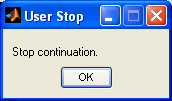
\includegraphics[scale=\scalefactor]{./fig/UserStop}
\label{fig:userstop}
\caption{Dialog box to interrupt a continuation process.}
\end{figure}
\begin{figure}
\centering
\includegraphics[scale=\scalefactor]{./fig/BasicMoMContinuationPath}
\label{fig:basicmomcontsol}
\caption{The stable saddle path of the equilibrium at the origin (green) spirals out from an unstable node (blue).}
\end{figure}

An important aspect of the calculation of stable-paths in \OCMAT\ is the possibility to handle constraints that become active on parts of the trajectory. First of all this means that possible violations of constraints have to be detected during the continuation. Secondly it is necessary to use the information about constraint violations to adapt the underlying \BVP\ and solution to restart the continuation process taking the active constraints into account.
\begin{matlab}
function solp=partialarc(sol,partarccoord)(*@\index{Command!continuation!\lstinline+partialarc+|indexbf}@*)
%
% PARTIALARC returns a part of a trajectory
%
% PARTIALARC(SOL,PARTARCCOORD) the arc of the solution structure SOl is
% returned for the indices specified by PARTARCCOORD.
%
% SOLP=PARTIALARC(SOL,PARTARCCOORD) SOLP is a solution structure, with
% adapted fields 'x', 'y', 'arcarg', 'arcinterval', 'arcposition'.
\end{matlab}
\begin{matlab}
function sol=addarc(sol,arc,iposition)(*@\index{Command!continuation!\lstinline+addarc+|indexbf}@*)
%
% ADDARC fit an arc into a solution
%
% ADDARC(SOL,ARC) the input arguments SOL and ARC are OCMat solution
% structures. ARC is placed as a new arc in front of SOL.
\end{matlab}
\paragraph{Example}
\begin{matlab}
>> m=stdocmodel('fishery2D');
>> ocEP=calcep(m);b=isadmissible(ocEP,m,[],'UserAdmissible');ocEP(~b)=[];store(m,ocEP);
>> opt=setocoptions('OCCONTARG','MaxStepWidth',1);
>> sol=initocmat_AE_EP(m,ocEP{2},1:2,[0.01 0.1],opt);
>> c=bvpcont('extremal2ep',sol,[],opt);
first solution found
tangent vector to first solution found

 Continuation step No.: 1
 stepwidth: 0.01
 Newton Iterations: 1
 Mesh size: 42
 Continuation parameter: 0.00567166

 Continuation step No.: 21
 stepwidth: 1
 Newton Iterations: 1
 Mesh size: 120
 Continuation parameter: 0.902635
 
Non admissible solution detected, reduce stepwidth.

 Continuation step No.: 22
 stepwidth: 0.5
 Newton Iterations: 1
 Mesh size: 131
 Continuation parameter: 0.915318

Non admissible solution detected, reduce stepwidth.
Current step size too small (point 29)

 Continuation step No.: 29
 stepwidth: 1e-005
 Newton Iterations: 1
 Mesh size: 131
 Continuation parameter: 0.915442

>> store(m,'extremal2ep');ocAsym=extremalsolution(m);

>> trj=partialarc(ocAsym{1},[1 1]);trj.arcarg=1;
>> ocAsymN=addarc(ocAsym{1},trj);

>> sol=initocmat_AE_AE(m,ocAsymN,1:2,[0.01 0.1],opt);
>> c=bvpcont('extremal2ep',sol,[],opt);
\end{matlab}

\subsection{Indifference Threshold}
The phenomenon that the optimal solution may not be unique is a well known phenomenon. In the large majority of cases the calculation and detection of these solutions needs to be done numerically. One of the strengths of \OCMAT\ is exactly this task, which in general (for models with at least two states) consists of two basic steps.
\begin{enumerate}
	\item The detection of an indifference threshold.
	\item The continuation of the detected indifference threshold, yielding a curve, surface, ....
\end{enumerate}
These basic steps are reflected in the actual implementation. For the detection of an indifference threshold \OCMAT\ provides the function \lstinline+findindifferencepoint+.
\begin{matlab}
function [indiffpt o]=findindifferencepoint(ocObj,sliceman1,sliceman2,varargin)(*@\index{Command!stdocmodel!\lstinline+findindifferencepoint+|indexbf}@*)
%
% FINDINDIFFERENCEPOINT find indifference threshold.
%
% FINDINDIFFERENCEPOINT(OCOBJ,IDX1,IDX2) IDX1 and IDX2 are the indices of
% continuation results stored in OCOBJ. To detect an indifference threshold
% the Hamiltonian is evaluated at the initial points of the continuation
% process (slice manifold) and intersected. The slice manifold is only
% considered from the first point to the point where it bends back, if it
% bends back at all.
%
% FINDINDIFFERENCEPOINT(OCOBJ,SLMF1,SLMF2) SLMF1 and SLMF2 are slice
% manifolds.
%
% FINDINDIFFERENCEPOINT(OCOBJ,IDX1,IDX2,OPT) 
%   OPT.GENERAL.AdmissibleTolerance defines the tolerance for the
%           collinearity test of the slice manifolds.  
%   OPT.OCCONTARG.PlotCont='on'/'off' if set 'on' the result is shown
%           graphically
%
% FINDINDIFFERENCEPOINT(OCOBJ,IDX1,IDX2,OPT,SPEC1,SPEC2) the argument
%       SPEC1= ''/'r': if set to 'r' the slice manifold is considered in
%               reverse order. This argument is useful if the threshold
%               point separates two solutions converging to the same limit
%               set. In that case it suffices to compute one slice manifold
%               (with at least two limit points) IDX and call
%               FINDINDIFFERENCEPOINT(OCOBJ,IDX,IDX,[],'r')
%
% INDIFFPT=FINDINDIFFERENCEPOINT(...) if the Hamiltonian functions
% intersect the (state) values of the intersection point INDIFFPT is
% returned otherwise it is empty.
%
% [INDIFFPT O]=FINDINDIFFERENCEPOINT(...) O is the corresponding obective
% value or empty.
\end{matlab}
This solution is used to initialize an indifference threshold continuation.
\begin{matlab}
function sol=initocmat_AE_IS(ocObj,ocMP,targetcoordinate,targetvalue,opt,fixedcoordinate,varargin)(*@\index{Command!stdocmodel!\lstinline+initocmat_AE_IS+|indexbf}@*)
%
% INITOCMAT_AE_IS initialization for the continuation of an indifference
% threshold
%
% SOL=INITOCMAT_AE_IS(OCOBJ,OCMP,TARGETCOORDINATE,TARGETVALUE) the
% continuation of an indifference threshold in the state space is
% initialized.    
% OCOBJ          ... corresponding optimal control model
% OCMP           ... two cell array of ocasymptotics, for the different
%                    solution paths or an instance of an ocmultipath
%                    object. 
% TARGETCOORDINATE ... the continuation is done along the n-1 coordinates
%                   (n number of states) 
% TARGETVALUE    ... The value of the target vector for the n-1
%                   coordinates.
%
% The output argument SOL is a solution structure for a BVP with the
% standard fields 'x', 'y', 'parameters' (MATLAB syntax for BVPs).
% The (important) OCMat specific fields 
%   arcinterval ... truncation of the time interval
%   arcarg      ... arc identifier for a specific combination of active and
%                   inactive constraints.
% are provided as well.
%
% During the initialization two global variables OCMATCONT and OCMATINDIF
% are initialized. The first variable contains general information for the
% continuation process. The second variable contains problem specific
% information.
%
% SOL=INITOCMAT_AE_IS(OCOBJ,OCMP,TARGETCOORDINATE,TARGETVALUE,OPT)
\end{matlab}
\paragraph{Example}
The following example is explained more detailed in \cref{sec:initandnumanacrm}.
\begin{matlab}
>> m=stdocmodel('harvest3D');
>> m=changeparametervalue(m,'r,l,s,w',[0.1 1 0.325 0]);
>> ocEP=calcep(m);b=isadmissible(ocEP,m,[],'UserAdmissible');ocEP(~b)=[];(*@\index{Command!stdocmodel!calcep}\index{Command!dynprimitive!isadmissible}@*)
>> [b dim]=issaddle(ocEP{:});ocEP(~b)=[];store(m,ocEP);(*@\index{Command!dynprimitive!issaddle}@*)
>> opt=setocoptions('OCCONTARG','MaxStepWidth',1,'GENERAL','BVPMethod','bvp6c');
>> opt=setocoptions(opt,'OCCONTARG','MaxContinuationSteps',100);
>> sol=initocmat_AE_EP(m,ocEP{1},1:3,ocEP{2}.y(1:3),opt,'TruncationTime',1000);
>> c=bvpcont('extremal2ep',sol,[],opt);
>> store(m,'extremal2ep');
>> opt=setocoptions(opt,'OCCONTARG','MaxStepWidth',50);
>> sol=initocmat_AE_EP(m,ocEP{2},1:3,ocEP{1}.y(1:3),opt,'TruncationTime',1000);
>> c=bvpcont('extremal2ep',sol,[],opt);
>> store(m,'extremal2ep');
>> ocAsym=extremalsolution(m);
>> trj=partialarc(ocAsym{2},[1 1]);trj.arcarg=1;
>> ocAsymN=addarc(ocAsym{2},trj);
>> sol=initocmat_AE_AE(m,ocAsymN,1:3,ocEP{1}.y(1:3),opt);
>> c=bvpcont('extremal2ep',sol,[],opt);
>> store(m,'extremal2ep');
>> it=findindifferencepoint(m,1,3);
>> sol=initocmat_AE_AE(m,ocAsymN,1:3,it,opt);
>> c=bvpcont('extremal2ep',sol,[],opt);
>> store(m,'extremal2ep');
>> sol=initocmat_AE_EP(m,ocEP{1},1:3,it,opt,'TruncationTime',1000);
>> c=bvpcont('extremal2ep',sol,[],opt);
>> store(m,'extremal2ep');
>> ocAsym=extremalsolution(m);
>> opt=setocoptions('OCCONTARG','InitStepWidth',0.1,'MaxStepWidth',5);
>> opt=setocoptions(opt,'SBVPOC','BCJacobian',0,'FJacobian',0);
>> opt=setocoptions(opt,'GENERAL','BVPMethod','bvp4c');
>> sol=initocmat_AE_IS(m,ocAsym(4:5),[1 2],[1.5 it(2)],opt);
>> c=bvpcont('indifferencesolution',sol,[],opt);
>> store(m,'indifferencesolution');
>> sol=initocmat_AE_IS(m,ocAsym(4:5),[3 2],[0.1 it(2)],opt,2);
>> c=bvpcont('indifferencesolution',sol,[],opt);
>> store(m,'indifferencesolution');
\end{matlab}
\section{General Commands}
\subsection{Auxiliary Tools}
A simple tool to help you to keep track of model specific notes, commands, etc...
\begin{matlab}
function fidwrite=remark(ocObj,varargin)(*@\index{Command!stdocmodel!\lstinline+remark+|indexbf}@*)
%
% REMARK creates or opens a text file for remarks.
%
% REMARK(OCOBJ) creates a file with the basic filename of the model OCOBJ,
% see ocmat/tools/remark for further information.
\end{matlab}
Called with a \lstinline+stdocmodel+ as argument a file with standard name, e.g., for \MoM\ \lstinline+momRemark.ocr+ is created or opened in the default data folder of the model \lstinline+\ocmat\model\usermodel\mom\data+. This command is more flexible implemented in the \lstinline+tools+ folder.
\begin{matlab}
function fidwrite=remark(basicfilename,folder,varargin)(*@\index{Command!tools!\lstinline+remark+|indexbf}@*)
%
% REMARK creates or opens a text file for remarks.
%
% REMARK(FNAME) the name of text file is given by the basic filename FNAME
% appending Remark and the extension 'ocr'. This file is created or opened
% if it already exists in the current directory. The actual date is
% appended at the end of the file. On a 'PC' it is opened with a user
% specified editor, if the extension is known to the system, e.g,
% Notepad++, or the MATLAB editor in any other cases. This command shall
% help the user to make model specific notes during her/his analysis.
%
% REMARK(FNAME,FOLDER) with FOLDER a specific folder for the file can be
% specified.
%
% REMARK(FNAME,FOLDER,TYPE) the TYPE specifies the extension of the file.
%   TYPE 
%       'standardmodel'         : 'ocr' 
%       'uncontrolledodemodel'  : 'odr' 
%       'spacedistributedmodel' : 'pdr' 
% and 'txt' otherwise.        
%
% FIDWRITE=REMARK(...) the file identifier FIDWRITE is returned.
\end{matlab}
The current \MATL\ \lstinline+history+ file can be appended to a model specific history file.
\begin{matlab}
function history(ocObj)(*@\index{Command!stdocmodel!\lstinline+history+|indexbf}@*)
%
% HISTORY appends current history file to model specific history file
%
% HISTORY(OCOBJ) creates or opens a file '[modelname]History.m' in the
% default model data folder and appends current MATLAB history file.
%
% HISTORY(OCOBJ,'OPEN') opens the history file '[modelname]History.m' in
% the MATLAB editor.
\end{matlab}
If you only want to store specific commands these can automatically be written into a model specific diary file.
\begin{matlab}
function diary(ocObj,flag)(*@\index{Command!stdocmodel!\lstinline+diary+|indexbf}@*)
%
% DIARY toggles model diary file on/off
%
% DIARY(OCOBJ) writes to the model specific diary file
% '[modelname]Diary.m' in the model data folder. New commands are appended
% to an already existing diary file. Calling DIARY(OCOBJ) a second time
% turns the diary modus off.
\end{matlab} 
\subsection{Option Handling}
\begin{matlab}
function opts=setocoptions(varargin)(*@\index{Command!options!\lstinline+setocoptions+|indexbf}@*)
%
% SETOCOPTIONS lets you adjust the options of the OCMAT toolbox.
%
% OPT=SETOCOPTIONS(CAT1,NAME1,VALUE1,CAT2,NAME2,VALUE2,...) replaces the
% values of the options NAME1, NAME2,... in the categories CAT1,CAT2,.. of
% the default option structure with new values VALUE1, VALUE2,... and
% returns an option structure OPT with the changed options.
%
% OPT=SETOCOPTIONS(OPS,CAT1,NAME1,VALUE1,CAT2,NAME2,VALUE2,...) replaces
% the values of the options NAME1, NAME2,... in the categories CAT1,CAT2,..
% of the option structure OPT with new values VALUE1, VALUE2,... and
% returns the option structure OPT with the changed options. 
%
% OPT=SETOCOPTIONS(OPT,CAT1,NAME1,VALUE1,NAME2,VALUE2,CAT2,NAME3,VALUE3,..)
% replaces the values of the options NAME1, NAME2, ... of the category CAT1
% of the (optional) option structure OPT with the values VALUE1 and VALUE2
% and option NAME3 of category CAT2 with value VALUE3 etc. and returns
% the changed option structure OPT.
\end{matlab}
\paragraph{Example}
\begin{matlab}
>> opt=setocoptions('OCCONTARG','MaxStepWidth',2,'GENERAL','BVPMethod','bvp5c');
\end{matlab}
where one sets the option \lstinline+MaxStepWidth+ to $2$ and \lstinline+BVPMethod+ to \lstinline+bvp5c+.

\begin{matlab}
function varargout = getocoptions(varargin)(*@\index{Command!options!\lstinline+getocoptions+|indexbf}@*)
%
% GETOCOPTIONS returns the value of the options defined in varargin
%
% [VALUE1 VALUE2 ...]=GETOCOPTIONS(CAT1,NAME1,CAT2,NAME2,...) returns the
% default values of the options with the named NAME1, NAME2,... located in
% the categories CAT1,CAT2,.. 
%
% [VALUE1 VALUE2 ...]=GETOCOPTIONS(CAT1,NAME1,DEFAULTVALUE1,CAT2,NAME2,...)
% returns the default values of the options with the named NAME1, NAME2,...
% located in the categories CAT1,CAT2,.. . If the default values are empty
% the optional input argument defaultvalue assigns an alternative value to
% this option. This default value does not have to be assigned for every
% option that is to be returned.
%
% [VALUE1 VALUE2 ...]=GETOCOPTIONS(OPT,CAT1,NAME1,CAT2,NAME2,...) returns the
% value of the options with the names NAME1,NAME2,... of the categories
% CAT1,CAT2,... of the option structure OPT.
%
% [VALUE1 VALUE2 ...]=GETOCOPTIONS(OPTS,CAT1,NAME1,DEFAULTVALUE1,CAT2,NAME2,...)
% returns the value of the options with the names NAME1,NAME2,... of the
% categories CAT1,CAT2,... of the option structure OPT. To avoid an empty
% output argument one can assign default values that are returned in case
% the required value of the option is empty in this option structure.
%
% [VALUE1 VALUE2 ...]=GETOCOPTIONS(OPTS,CAT1,NAME1,DEFAULTVALUE1,NAME2,CAT2,...)
% returns the value of the options with the names name1,name2,... of the
% categorie CAT1 of the option structure OPT. To avoid an empty
% output argument one can assign default values that are returned in case 
% the required value of the option is empty in this option structure.
\end{matlab}
\paragraph{Example}
\begin{matlab}
>> [bvpsolver n]=getocoptions('GENERAL','BVPMethod','TrivialArcMeshNum');
\end{matlab}
assigns the values of the options \lstinline+BVPMethod+ and \lstinline+TrivialArcMeshNum+ of the category \lstinline+GENERAL+ of the default option structure to the variables \lstinline+bvpsolver+ and \lstinline+n+.
\begin{matlab}
function showocoptions(varargin)(*@\index{Command!options!\lstinline+showocoptions+|indexbf}@*)
%
% SHOWOCOPTIONS is a function to display the available categories, names and
% values of an option structure.
%
% SHOWOCOPTIONS shows the default options.
%
% SHOWOCOPTIONS(OPTS) displays the options of the option structure OPTS.
% 
% SHOWOCOPTIONS(CAT) displays the content of the option category CAT of
% the default options
%
% SHOWOCOPTIONS(OPTS,CAT) displays the content of the option category CAT
% of the option structure OPTS.
\end{matlab}
\paragraph{Example}
\begin{matlab}
>> showocoptions('INIT')
INIT
~~~~
             Simplify: 'n'
             Jacobian: 'explicit'
      ControlDynamics: 'explicit'
    ParameterJacobian: 'explicit'
                Force: 'off'
       MessageDisplay: 'off'
      TestConsistency: 'on'
\end{matlab}
\begin{matlab}
function opts=loadocoptions(filename,varargin)(*@\index{Command!options!\lstinline+loadocoptions+|indexbf}@*)
%
% LOADOCOPTIONS An option structure that has priorily been saved to the
% file filename will be loaded.
%
% OPTS=LOADOCOPTIONS(FILENAME) The option structure contained in FILENAME,
% located at the defaultpath at data/options/ will be returned in the
% option structure OPTS.  
%
% OPTS=LOADOCOPTIONS(FILENAME,PATH) The option structure contained in
% FILENAME, located at the PATH defined in the input arguments will be
% returned in the option structure OPTS. 
\end{matlab}

\section{Plotting Commands}
\label{sec:plot_command_sel_com}
In this section plotting commands are introduced. These commands base on the class structure defined in \OCMAT. Their main purpose is it to facilitate the graphical depiction of numerical results done within \OCMAT. Even though these plotting commands are very flexible they cannot cover every possible situation. Therefore, these commands should be seen as an offer. Certainly the user can utilize the native \MATL\ plotting commands.

The low level plotting command is the \lstinline+line+ command.
\begin{matlab}
function varargout=line(ocTrj,varargin)(*@\index{Command!octrajectory!\lstinline+line+|indexbf}@*)
%
% LINE basic plot command of an octrajectory.
%
% LINE(OCTRJ,XCOORD,YCOORD) OCTRJ is an instance of the class octrajecotry
% and XCOORD, YCOORD, respectively coordinates of the dependent variables
% of OCTRJ. This commands calls the native line command of MATLAB with:
%   LINE(OCTRJ.Y(XCOORD,:),OCTRJ.Y(YCOORD,:))
% For a detailed description of the LINE command see the MATLAB help.
%
% LINE(OCTRJ,XCOORD,YCOORD,ZCOORD) creates a 3D plot using a third
% coordinate ZCOORD. 
%
% LINE(OCTRJ,XCOORD,YCOORD,(ZCOORD),'PROPERTYNAME',PROPERTYVALUE,...)
% additionally usual line properties can be provided.
%
% LINE(OCTRJ,'XDATA',XDATA,'XCOORD',XCOORD,'YDATA',YDATA,'YCOORD',YCOORD,'Z
% DATA',ZDATA,'ZCOORD',ZCOORD,'PROPERTYNAME',PROPERTYVALUE,...) is the full
% version of the LINE command, with paired arguments. 'XDATA', 'YDATA' and
% optionally 'ZDATA' denote the name of the depicted variables. Possible
% values are:
%   'dependentvar' ... dependent variables of OCTRJ, usually state and
%                      costates
%   'independentvar' ... the independent variable of OCTRJ, usually the
%                      time
% If model specific variables are depicted, e.g., state, control,
% Hamiltonian, etc. the OCOBJ instance of the model has to be provided as
% well, by the paired argument 'OCMODEL',OCOBJ. Allowed values for 'XDATA',
% 'YDATA' and optionally 'ZDATA' are: 
%   'state'
%   'costate',
%   'control'
%   'lagrangemultiplier'
%   'canonicalsystem'
%   'hamiltonian'
%   'userfunction'
%
% LINE(OCTRJ,...,'CONNECT',VAL,...) for VAL=0 (default) each arc is plotted
% separately, for VAL=1 all arcs are combined.
%
% H=LINE(...) returns the line handles H  for the plotted arc(s).
\end{matlab}
The \lstinline+plot+ command is the ``high level'' counterpart to the \lstinline+line+ command.
\begin{matlab}
function varargout=plot(varargin)(*@\index{Command!octrajectory!\lstinline+plot+|indexbf}@*)
%
% PLOT plot command for an octrajectory.
%
% PLOT(OCTRJ,COORD) plots the coordinates COORD (integer vector) of the
% dependent variables of the octrajectory OCTRJ against the independent
% variable.
%
% PLOT(OCTRJ,XCOORD,YCOORD) plots the coordinates XCOORD and YCOORD of
% the dependent variables of the octrajectory OCTRJ. XCOORD or YCOORD can
% be an integer vector.
%
% PLOT(OCTRJ,COORD,'YDATA',YDATA,'OCMODEL',OCOBJ) 
%   'YDATA'  : specifies the plotted terms. Default value is
%              'dependentvar'. For a detailed list see the LINE command.
%   'OCMODEL': OCOBJ is an object of the used model class. These only have
%              to be provided if model specific terms, e.g. state, costate,
%              control, ... are used for 'YDATA'
%
% PLOT(OCTRJ,XCOORD,YCOORD,'XDATA',XDATA,'YDATA',YDATA,'OCMODEL',OCOBJ) 
%   'XDATA'/'YDATA'  : specifies the plotted terms. Default value is
%                      'dependentvar'. For a detailed list see the LINE
%                      command. 
%   'OCMODEL': OCOBJ is an object of the used model class. These only have
%              to be provided if model specific terms, e.g. state, costate,
%              control, ... are used for 'XDATA' or 'YDATA'.
%  
% PLOT(AHANDLE,...) plots into the axes with the handle AHANDLE instead of
% into the current axes (gca)
% plots to the axes with AHANDLE.
%  
% PLOT(...,'CONNECT',CONNECTVAL,...) CONNECTVAL : 0 (default)|1. For 0
% different arcs of the octrajectory OCTRJ are plotted as separate lines.
% For 1 different arcs are combined into a single line.
% 
%  
% PLOT(...'PROPERTYNAME',PROPERTYVALUE,...) sets properties to the
% specified property values for all lineseries graphics objects created by
% PLOT. 
%
% H=PLOT(...) returns a column vector of handles to lineseries graphics
% objects, one handle per line. 
\end{matlab}
\begin{matlab}
function varargout=plot3(varargin)(*@\index{Command!octrajectory!\lstinline+plot3+|indexbf}@*)
%
% PLOT3 3D plot command for an octrajectory.
%
% PLOT3(OCTRJ,XCOORD,YCOORD) plots the coordinates XCOORD and YCOORD of
% the dependent variables of the octrajectory OCTRJ against the independent
% variable. XCOORD and YCOORD have to be single valued..
%
% PLOT3(OCTRJ,XCOORD,YCOORD,'XDATA',XDATA,'YDATA',YDATA,'OCMODEL',OCOBJ) 
%   'XDATA'/'YDATA'  : specifies the plotted terms. Default value is
%                      'dependentvar'. For a detailed list see the LINE
%                      command. 
%   'OCMODEL': OCOBJ is an object of the used model class. These only have
%              to be provided if model specific terms, e.g. state, costate,
%              control, ... are used for 'XDATA' or 'YDATA'.
%  
% PLOT3(AHANDLE,...) plots into the axes with the handle AHANDLE instead of
% into the current axes (gca)
% plots to the axes with AHANDLE.
%  
% PLOT3(...,'CONNECT',CONNECTVAL,...) CONNECTVAL : 0 (default)/1. For 0
% different arcs of the octrajectory OCTRJ are plotted as separate lines.
% For 1 different arcs are combined into a single line.
% 
%  
% PLOT3(...'PROPERTYNAME',PROPERTYVALUE,...) sets properties to the
% specified property values for all lineseries graphics objects created by
% PLOT3. 
%
% H=PLOT3(...) returns a column vector of handles to lineseries graphics
% objects, one handle per line. 
\end{matlab}
\paragraph{Example}
To load the models for the following examples it is assumed that the current working directory of \MATL\ is the \OCMAT\ directory. The models are located in the documentation folder of \OCMAT\ (\lstinline+'ocmat/doc/latex/matlab/data'+).
\begin{matlab}
>> m=stdocmodel('harvest3D');
>> load(m,[],1,'MultiHarvest3D','./doc/latex/matlab/data')
>> ocAsym=extremalsolution(m);
>> line(ocAsym{4},'xcoord',1,'ycoord',1:3,'xdata','independentvar','ydata','dependentvar')
>> plot(ocAsym{4},1:3)(*@, see \cref{fig:multipleharvest3Didv}@*)
>> line(ocAsym{4},'xcoord',1,'ycoord',1:3,'xdata','time','ydata','state','ocmodel',m)
>> plot(ocAsym{4},1,1:3,'xdata','time','ydata','state','ocmodel',m)(*@, see \cref{fig:multipleharvest3Dtcv}@*)
>> plot(ocAsym{4},1,1,'xdata','time','ydata','control','ocmodel',m)(*@, see \cref{fig:multipleharvest3Dtcv}@*)
>> line(ocAsym{4},'xcoord',1,'ycoord',2,'zcoord',3,'xdata','dependentvar', ...
         'ydata','dependentvar','zdata','dependentvar'),view(3)
>> plot3(ocAsym{4},1,2,3);view(3)(*@, see \cref{fig:multipleharvest3Ddvs}@*)
>> plot3(ocAsym{4},1,2,3,'connect',1);view(3)
>> plot3(ocAsym{4},1,2,1,'xdata','state','ydata','state','zdata','hamiltonian','ocmodel',m),view(3)
\end{matlab}
\begin{figure}
\centering
\includegraphics[scale=\scalefactor]{./fig/MultiHarvest3DIndependent-DependentVar}
\caption{The \lstinline+line+ and \lstinline+plot+ command depicting the first three coordinates of a \BVP\ solution.}
\label{fig:multipleharvest3Didv}
\end{figure}
\begin{figure}
\centering
\includegraphics[scale=\scalefactor]{./fig/MultiHarvest3DTime-StateVar}
\caption{The \lstinline+line+ and \lstinline+plot+ command depicting the time paths of the states.}
\label{fig:multipleharvest3Dtsv}
\end{figure}
\begin{figure}
\centering
\includegraphics[scale=\scalefactor]{./fig/MultiHarvest3DTime-ControlVar}
\caption{The \lstinline+line+ and \lstinline+plot+ command depicting the time path of the control.}
\label{fig:multipleharvest3Dtcv}
\end{figure}
\begin{figure}
\centering
\includegraphics[scale=\scalefactor]{./fig/MultiHarvest3DDependentSpaceVar}
\caption{The \lstinline+line+ and \lstinline+plot3+ command depicting the solution in the dependent variable space.}
\label{fig:multipleharvest3Ddvs}
\end{figure}
\begin{figure}
\centering
\includegraphics[scale=\scalefactor]{./fig/MultiHarvest3DCostateSpaceVar}
\caption{The \lstinline+line+ and \lstinline+plot+ command depicting the solution in the costate space.}
\label{fig:multipleharvest3Dcss}
\end{figure}
\begin{matlab}
function varargout=plotcont(varargin)(*@\index{Command!stdocmodel!\lstinline+plotcont+|indexbf}@*)
%
% PLOTCONT plots the result(s) of a continuation process
%
% PLOTCONT(OCOBJ,'XDATA',XCOORD,'YDATA',YCOORD) plots for each continuation
% process of class 'extremal' stored in OCOBJ the last detected solution
% (entry of the ExtremalSolution field). The values of the x/y-axis are
% determined by the coordinate XCOORD/YCOORD of the term specified in
% 'XDATA'/'YDATA'. Possible values for 'XDATA' and 'YDATA' are: 
%
%   'independentvar'
%   'time'
%   'dependentvar'
%   'state'
%   'costate',
%   'control'
%   'lagrangemultiplier'
%   'canonicalsystem'
%   'hamiltonian'
%   'userfunction'
% 
% The values of XCOORD and YCOORD specify the coordinates of the
% corresponding terms. Either XCOORD or YCOORD can be a vector.
%
% PLOTCONT(...,'PROPERTYNAME',PROPERTYVALUE,...) 
% OCMAT specific pairs 'PROPERTYNAME',PROPERTYVALUE are:
%   'contclass' : 'extremal' continuation of extremal solutions
%                 'indifferencesolution' continuation of indifference
%                                        thresholds 
%   'contfield' : 'ExtremalSolution' last computed solution of a
%                 continuation process  
%                 'ContinuationSolution' solutions computed during the
%                 continuation process.  
%   'index'     : number(s) specifying the continuation process for which
%                 the solution(s) are plotted.
%   'connect'   : (0)/1 see stdocmodel/plot.
% The following values for 'PROPERTYNAME' have only an effect if the
% 'contfield' is set to 'ContinuationSolution'
%   'contindex' : a vector that specifies the indices of solutions that are
%                 plotted.
%   'hold'      : if set to 'on' the axis property 'NextPlot' is set to
%                 'add' during the plotting of the results of the
%                 continuation process. 
%               : if set to 'off' the axis property 'NextPlot' is set to
%                 'replace' during the plotting of the results of the
%                 continuation process. 
%
% For 'PROPERTYNAME' and PROPERTYVALUE usual axes properties can be
% provided.
%
% PLOTCONT(AHANDLE,...) plots into the axes with the handle AHANDLE instead
% of into the current axes (gca)
%
% H=PLOTCONT(...) returns a column vector of handles to lineseries graphics
% objects, one handle per line. 
\end{matlab}
The next class of plotting commands depict result already stored in an instance of the \lstinline+stdocmodel+ class and therefore facilitates the graphical display.
\begin{matlab}
function varargout=plot3cont(varargin)(*@\index{Command!stdocmodel!\lstinline+plot3cont+|indexbf}@*)
%
% PLOT3CONT 3D plot of the result(s) of a continuation process
%
% PLOT3CONT(OCOBJ,'XDATA',XCOORD,'YDATA',YCOORD,'ZDATA',ZCOORD) plots for
% each continuation process of class 'extremal' stored in OCOBJ the last
% detected solution (entry of the ExtremalSolution field). The values of
% the x/y/z-axis are determined by the coordinate XCOORD/YCOORD/ZCOORD of
% the term specified in 'XDATA'/'YDATA'/'ZDATA'. Possible values for
% 'XDATA', 'YDATA' and 'ZDATA' are:  
%
%   'independentvar'
%   'time'
%   'dependentvar'
%   'state'
%   'costate',
%   'control'
%   'lagrangemultiplier'
%   'canonicalsystem'
%   'hamiltonian'
%   'userfunction'
% 
% The values of XCOORD, YCOORD, ZCOORD specify the coordinates of the
% corresponding terms.
%
% PLOT3CONT(...,'PROPERTYNAME',PROPERTYVALUE,...) 
% OCMAT specific pairs 'PROPERTYNAME',PROPERTYVALUE are:
%   'contclass' : 'extremal' continuation of extremal solutions
%                 'indifferencesolution' continuation of indifference
%                                        thresholds 
%   'contfield' : 'ExtremalSolution' last computed solution of a
%                 continuation process  
%                 'ContinuationSolution' solutions computed during the
%                 continuation process.  
%   'index'     : number(s) specifying the continuation process for which
%                 the solution(s) are plotted.
%   'connect'   : (0)/1 see stdocmodel/plot.
%   'view3d'    : 'on' sets the default three-dimensional view 
%                 'off' uses the view specified by the axis properties.  
% The following values for 'PROPERTYNAME' have only an effect if the
% 'contfield' is set to 'ContinuationSolution'
%   'contindex' : a vector that specifies the indices of solutions that are
%                 plotted.
%   'hold'      : if set to 'on' the axis property 'NextPlot' is set to
%                 'add' during the plotting of the results of the
%                 continuation process. 
%               : if set to 'off' the axis property 'NextPlot' is set to
%                 'replace' during the plotting of the results of the
%                 continuation process. 
%
% For 'PROPERTYNAME' and PROPERTYVALUE usual axes properties can be
% provided.
%
% PLOT3CONT(AHANDLE,...) plots into the axes with the handle AHANDLE
% instead of into the current axes (gca) 
%
% H=PLOT3CONT(...) returns a column vector of handles to lineseries
% graphics objects, one handle per line. 
\end{matlab}
Beside the results of a continuation process it is also possible to directly address limitsets (equilibria, limitcycles).
\begin{matlab}
function varargout=plotlimitset(varargin)(*@\index{Command!stdocmodel!\lstinline+plotlimitset+|indexbf}@*)
%
% PLOTLIMITSET plots the stored limitsets
%
% PLOTLIMITSET(OCOBJ,'XDATA',XCOORD,'YDATA',YCOORD) plots the equilibria
% stored in OCOBJ. The values of the x/y-axis are determined by the
% coordinate XCOORD/YCOORD of the term specified in 'XDATA'/'YDATA'.
% Possible values for 'XDATA' and 'YDATA' are:  
%
%   'independentvar'
%   'time'
%   'dependentvar'
%   'state'
%   'costate',
%   'control'
%   'lagrangemultiplier'
%   'canonicalsystem'
%   'hamiltonian'
%   'userfunction'
% 
% The values of XCOORD and YCOORD specify the coordinates of the
% corresponding terms. Either XCOORD or YCOORD can be a vector.
%
% PLOTLIMITSET(...,'PROPERTYNAME',PROPERTYVALUE,...) 
% OCMAT specific pairs 'PROPERTYNAME',PROPERTYVALUE are:
%   'limitclass': 'equilibrium' the equilibria stored in the result field
%                 'Equilibrium'
%   'index'     : integer vector specifying the index of the limitsets that
%                 are plotted. 
%
% For 'PROPERTYNAME' and PROPERTYVALUE usual axes properties can be
% provided.
%
% PLOTLIMITSET(AHANDLE,...) plots into the axes with the handle AHANDLE
% instead of into the current axes (gca)
%
% H=PLOTLIMITSET(...) returns a column vector of handles to lineseries
% graphics objects, one handle per line. 
\end{matlab}
\begin{matlab}
function varargout=plot3limitset(varargin)(*@\index{Command!stdocmodel!\lstinline+plot3limitset+|indexbf}@*)
%
% PLOT3LIMITSET plots the stored limitsets
%
% PLOT3LIMITSET(OCOBJ,'XDATA',XCOORD,'YDATA',YCOORD) plots the equilibria
% stored in OCOBJ. The values of the x/y/z-axis are determined by the
% coordinate XCOORD/YCOORD/ZCOORD of the term specified in
% 'XDATA'/'YDATA'/'ZDATA'. Possible values for 'XDATA', 'YDATA' and 'ZDATA' 
% are:   
%
%   'independentvar'
%   'time'
%   'dependentvar'
%   'state'
%   'costate',
%   'control'
%   'lagrangemultiplier'
%   'canonicalsystem'
%   'hamiltonian'
%   'userfunction'
% 
% The values of XCOORD, YCOORD and ZCOORD specify the coordinates of the
% corresponding terms.
%
% PLOT3LIMITSET(...,'PROPERTYNAME',PROPERTYVALUE,...) 
% OCMAT specific pairs 'PROPERTYNAME',PROPERTYVALUE are:
%   'limitclass': 'equilibrium' the equilibria stored in the result field
%                 'Equilibrium'
%   'index'     : integer vector specifying the index of the limitsets that
%                 are plotted. 
%   'view3d'    : 'on' sets the default three-dimensional view 
%                 'off' uses the view specified by the axis properties.  
%
% For 'PROPERTYNAME' and PROPERTYVALUE usual axes properties can be
% provided.
%
% PLOT3LIMITSET(AHANDLE,...) plots into the axes with the handle AHANDLE
% instead of into the current axes (gca)
%
% H=PLOT3LIMITSET(...) returns a column vector of handles to lineseries
% graphics objects, one handle per line. 
\end{matlab}
One of the advantages when using the previous plotting commands acting on the \lstinline+stdocmodel+ class is the assignment of a unique identifier to each line object. This identifier is a string, given by the \lstinline+continuationclass+ or \lstinline+limitclass+ and the corresponding index. It is assigned to the \lstinline+Tag+ property of the line object. To retrieve this information \lstinline+gettag+ can be used
\begin{matlab}
function [tag,objh] = gettag(varargin)(*@\index{Command!tools!\lstinline+gettag+|indexbf}@*)
%
% GETTAG reads out the 'TAG' property of lineseries graphics objects.
%
% OUT = GETTAG(N) reads out the 'TAG' property of N lineseries graphics
% objects. The lineseries graphics objects are marked using the mouse. If
% the lines are plotted with one of the OCMAT stdocmodel plotting commands
% (plotcont, plotlimitset, ...) the TAGs are unique names. The TAGs are
% returned in the cell array OUT.    
%
% GETTAG mainly bases on the MATLAB function GINPUT.
\end{matlab}
\paragraph{Example}
\begin{matlab}
>> m=stdocmodel('fishery2D');
>> load(m,[],1,'MultiFishery2D','doc/latex/matlab/data')
>> plotcont(m,'state',1,'state',2,'index',[1 3])(*@, see \cref{fig:multiplefishery2Dsp}@*)
>> hold on
>> plotlimitset(m,'state',1,'state',2,'Marker','.','MarkerSize',14,'index',[1 3]);
>> gettag(3)
ans =
ExtremalSolution_extremal2ep_Nr:3
ExtremalSolution_extremal2ep_Nr:1
Equilibrium_Nr:1                 
>> clf,plot3cont(m,'state',1,'state',2,'hamiltonian',1,'index',[1 3]);figure(gcf),view(3)
>> hold on(*@, see \cref{fig:multiplefishery2Dshp}@*)
>> plot3limitset(m,'state',1,'state',2,'hamiltonian',1,'Marker','.','MarkerSize',14,'index',[1 3]);
\end{matlab}
\begin{figure}
\centering
\includegraphics[scale=\scalefactor]{./fig/MultiFishery2DStateSpaceSolutions}
\caption{The last detected solutions of the first and third continuation process. Together with the first and third equilibrium. Depicted in the state space.}
\label{fig:multiplefishery2Dsp}
\end{figure}
\begin{figure}
\centering
\includegraphics[scale=\scalefactor]{./fig/MultiFishery2DStateSpaceHamiltonianSolutions}
\caption{The last detected solutions of the first and third continuation process. Together with the first and third equilibrium. Depicted in the state-Hamiltonian space.}
\label{fig:multiplefishery2Dshp}
\end{figure}


\chapter{Miscellaneous}
\label{ch:miscellaneous}
In the following sections diverse extensions of the general problem \cref{eq:simple_simple_opt_pro} are discussed.
\section{Implicit Optimal Control Values}
\label{sec:ImplicitOptimalControlValues}

\section{Non-autonomous Problem}
\label{sec:NonAutonomousProblem}

\section{Pure State Constraints}
\label{sec:PureStateConstraints}

\section{Diverging Solutions}
\label{sec:DivergingSolutions}

\section{\MATCONT\ Interface}
\label{sec:MATCONTInterface}

\section{Periodic Solutions}
\label{sec:PeriodicSolutions}

\section{\BVP\ Bifurcations}
\label{sec:BVPBifurcations}


\appendix
\chapter{Options}
\label{sec:options}
For many calculations it is necessary to include the possibility to specify options that determine the quality and the run-time of the results. In order to be able to easily access the options, \OCMAT\ provides several functions to make the option-handling as easy as possible. All of the available options can be accessed through a basic option structure. This structure consists of several fields (categories) containing different structures containing concrete options and their value needed for certain functions.
\section{\texorpdfstring{\lstinline+INIT+}{INIT}}
\label{sec:options_opts_init}
The category \lstinline+INIT+ contains options required during the model initialization process. The available options are

\begin{tabularx}{\linewidth}{|l|c|X|}\hline
\textbf{Name} & \textbf{Default Value} & \textbf{Description}\\\hline
\lstinline+Simplify+  &  \lstinline+'n'+   & Simplifies symbolic terms during model initialization.\\
%\lstinline+Jacobian+  &  \lstinline+'explicit'+   &\\
%\lstinline+ControlDynamics+  &  \lstinline+'explicit'+   &\\
%\lstinline+ParameterJacobian+  &  \lstinline+'explicit'+   &\\
%\lstinline+Force+  &  \lstinline+'off'+   &\\
\lstinline+MessageDisplay+  &  \lstinline+'off'+   & Displays messages during model initialization process.\\
\lstinline+TestConsistency+  &  \lstinline+'on'+   & Tests the formal consistency of the model initialization file.\\
\hline
\end{tabularx}

\section{\texorpdfstring{\lstinline+OCCONTARG+}{OCCONTARG}}
\label{sec:options_opts_occontarg}

The category \lstinline+OCCONTARG+ contains the options for the continuation process.

\begin{tabularx}{\linewidth}{|l|c|X|}\hline
\textbf{Name} & \textbf{Default Value} & \textbf{Description}\\\hline
\lstinline+Increment+ & \lstinline+1e-5+ & Increment for numerical derivations.\\ 
%\lstinline+MaxCorrIters+ & \lstinline+10+ & \\ 
\lstinline+MaxTestIters+ & \lstinline+10+ & Maximum number of iterations for test functions. (\lstinline+bvpcont+)\\ 
%\lstinline+FunTolerance+ & \lstinline+1e-6+ & \\ 
\lstinline+VarTolerance+ & \lstinline+1e-6+ & Distance tolerance. \\ 
\lstinline+MaxContinuationSteps+ & \lstinline+300+ &  Maximum number of continuation steps.\\ 
\lstinline+TestTolerance+ & \lstinline+1e-5+ & Deviation tolerance from zero.\\ 
\lstinline+Singularities+ & \lstinline+0+ & Test for singularities.\\ 
\lstinline+Backward+ & \lstinline+0+ & Start continuation: (0) direction of tangent, (1) opposite direction of tangent.\\ 
\lstinline+InitStepWidth+ & \lstinline+0.0100+ & Initial step width of continuation.\\ 
\lstinline+MaxStepWidth+ & \lstinline+0.1000+ & Maximum step width of continuation. \\ 
\lstinline+MinStepWidth+ & \lstinline+1e-5+ &  Minimum step width of continuation.\\ 
\lstinline+IncreaseFactor+ & \lstinline+1.3000+ & Factor for the increase of the step width.\\ 
\lstinline+DecreaseFactor+ & \lstinline+0.5000+ & Factor for the decrease of the step width. \\ 
\lstinline+ContinuationMethod+ & \lstinline+1+ &  Type of continuation algorithm: (0) pseudo-arclength, (1) Moore-Penrose\\ 
\lstinline+WorkSpace+ & \lstinline+0+ & \\ 
\lstinline+HitTargetValue+ & \lstinline+1+ & Tests (1) if user provided target value is hit, (0) no check for target value.\\ 
\lstinline+CheckAngle+ & \lstinline+0.9000+ & Maximum angle between tangents of two consecutive continuation steps.\\ 
\lstinline+CheckStep+ & \lstinline+3+ & Continuation step to start angle check. \\ 
\lstinline+SaveIntermediate+ & \lstinline+'on'+ & Save results during continuation process \lstinline+'on'+ or \lstinline+'off'+.\\ 
\lstinline+PrintContStats+ & \lstinline+'on'+ & Display information about continuation process at command window \lstinline+'on'+ or \lstinline+'off'+.\\ 
\lstinline+PlotCont+ & \lstinline+'on'+ & Plot result of continuation process \lstinline+'on'+ or \lstinline+'off'+.\\ 
\lstinline+IgnoreSingularity+ & \lstinline+[]+ & \\ 
\lstinline+ExitOnTargetValue+ & \lstinline+'on'+ & Exit (1) if user provided target value is hit, (0) no exit.\\ 
\lstinline+Locators+ & \lstinline+[]+ & \\ 
\lstinline+Userfunctions+ & \lstinline+0+ & \\ 
\lstinline+CheckAdmissibility+ & \lstinline+'on'+ & Check admissibility of solution during continuation process \lstinline+'on'+ or \lstinline+'off'+.\\ 
\lstinline+Adapt+ & \lstinline+3+ & Number of steps after which model specific adapt function is called.\\ 
\lstinline+TotalRelativeDistance+ & \lstinline+1+ & \\ 
\hline
\end{tabularx}

\section{\texorpdfstring{\lstinline+GENERAL+}{GENERAL}}
\label{sec:options_opts_general}

The category \lstinline+GENERAL+ contains general options for \OCMAT.

\begin{tabularx}{\linewidth}{|l|c|X|}\hline
\textbf{Name} & \textbf{Default Value} & \textbf{Description}\\\hline
\lstinline+BVPMethod+ & \lstinline+'bvp4c'+ & Possible \BVP\ methods are: \lstinline+'bvp4c'+, \lstinline+'bvp5c'+, \lstinline+'bvp6c'+.\\ 
\lstinline+ODESolver+ & \lstinline+'ode45'+ & A native \MATL\ \ODE\ solver or user defined \ODE\ solver.\\ 
\lstinline+NewtonSolver+ & \lstinline+'newtcorr4bvp'+ & The used Newton algorithm for a continuation step.\\ 
\lstinline+EquationSolver+ & \lstinline+'fsolve'+ & The numerical solver for the calculation of equilibria.\\ 
\lstinline+ZeroDeviationTolerance+ & \lstinline+1e-6+ & Tolerance for the deviation from zero.\\ 
\lstinline+AdmissibleTolerance+ & \lstinline+1e-6+ & Tolerance for admissibility.\\ 
\lstinline+ImaginaryTolerance+ & \lstinline+1e-010+ & Smaller imaginary parts are set to zero.\\ 
\lstinline+TrivialArcMeshNum+ & \lstinline+40+ & Number of discretization points for limitset solutions (equilibrium, periodic solution).\\ 
\lstinline+MultiPointBVP+ & \lstinline+'on'+ & If the used \BVP\ solver allow multi-point \BVPs, otherwise multi-point problems are transformed to two-point problems.\\ 
\hline
\end{tabularx}

\section{\texorpdfstring{\lstinline+NEWTON+}{NEWTON}}
\label{sec:options_opts_newton}

The category \lstinline+NEWTON+ contains options used for the used Newton solver for the continuation process.

\begin{tabularx}{\linewidth}{|l|c|X|}\hline
\textbf{Name} & \textbf{Default Value} & \textbf{Description}\\\hline
\lstinline+MaxNewtonIters+ & \lstinline+4+ & Maximum number of Newton iterations.\\ 
\lstinline+MaxProbes+ & \lstinline+4+ & Maximum iteration numbers of weak line search step.\\ 
\lstinline+AbsTol+ & \lstinline+1e-3+ & Maximum value of the absolute tolerance for the norm of the coefficient in the Newton step. \\ 
%\lstinline+RelTol+ & \lstinline+1e-3+ & \\ 
%\lstinline+Display+ & \lstinline+''+ & \\ 
%\lstinline+TRM+ & \lstinline+0+ & \\ 
%\lstinline+Log+ & \lstinline+0+ & \\ 
%\lstinline+LambdaMin+ & \lstinline+1e-3+ & \\ 
%\lstinline+UpdateJacFactor+ & \lstinline+0.5000+ & \\ 
%\lstinline+SwitchToFFNFactor+ & \lstinline+0.5000+ & \\ 
\hline
\end{tabularx}

\section{\texorpdfstring{\lstinline+SBVPOC+}{SBVPOC}}
\label{sec:options_opts_sbvpoc}

The category \lstinline+SBVPOC+ contains options specifically for the \BVP\ solver.

\begin{tabularx}{\linewidth}{|l|c|X|}\hline
\textbf{Name} & \textbf{Default Value} & \textbf{Description}\\\hline
\lstinline+MeshAdaptation+ & \lstinline+'on'+ & Sets the mesh adaptation of the BVP solver 'on' or 'off'.\\ 
\lstinline+MeshAdaptAbsTol+ & \lstinline+1e-6+ & The threshold for the mesh adaptation is given by the quotient of the absolute 'MeshAdaptAbsTol' and relative tolerance 'MeshAdaptRelTol'.\\ 
\lstinline+MeshAdaptRelTol+ & \lstinline+1e-5+ & \\ 
%\lstinline+MeshAdaptK+ & \lstinline+1000+ & \\ 
%\lstinline+MeshAdaptN0+ & \lstinline+100+ & \\ 
%\lstinline+MeshAdaptMaxIter+ & \lstinline+15+ & \\ 
%\lstinline+MeshAdaptFineMesh+ & \lstinline+1+ & \\ 
\lstinline+Vectorized+ & \lstinline+'on'+ & The function for the dynamics is vectorized ('on'), or not vectorized ('off').\\ 
\lstinline+NMax+ & \lstinline+1000+ & Maximum number of grid points of the BVP solution.\\ 
\lstinline+MaxNewPts+ & \lstinline+2+ & Maximum number of points that can be added during mesh adaptation per time interval.\\ 
\lstinline+FJacobian+ & \lstinline+1+ & Computes the function derivatives by user provided analytical expressions (1), numerical approximation (0)\\ 
\lstinline+BCJacobian+ & \lstinline+1+ & Computes the derivatives of the boundary conditions by user provided analytical expressions (1), numerical approximation (0)\\ 
%\lstinline+residualReductionGuard+ & \lstinline+1e-3+ & \\ 
\hline
\end{tabularx}

\section{\texorpdfstring{\lstinline+ODE+, \lstinline+BVP+, \lstinline+EP+}{\ODE, \BVP, EP}}
\label{sec:options_opts_odebvpep}

See \MATL-Help \lstinline+odeset+, \lstinline+bvpset+ and \lstinline+optimset+ (optimization toolbox required)


\section{\texorpdfstring{\lstinline+MATCONT+}{MATCONT}}
\label{sec:options_opts_matcont}

See \MATCONT-help to learn more about the option structure created with \lstinline+contset+. \MATCONT\ can be downloaded from \httpMATCONT


\chapter{Class Design}
\label{sec:classdesign}
\section{Model class}
In the current version of \OCMAT\ only the class \lstinline+stdocmodel+ is implemented. The implementation of further classes and extensions are planned, e.g. multi-stage \OCPRO s or space distributed \OCPRO s.

\subsection{Standard Model Class (\texorpdfstring{\lstinline+stdocmodel+}{stdocmodel})}\index{Classes!stdocmodel|indexbf}
Any instance \lstinline+ocObj+ of the class \lstinline+stdocmodel+ represents a model of type \cref{eq:simple_simple_opt_pro} specified for a given set of parameter values. To add a new model an initialization file has to be provided and processed, for examples see \cref{sec:InitializationMoM,sec:InitializationCRM}. 

This step only has to be done once. During the initialization of a new model the necessary \MATL\ files for a numerical analysis are created. These files are moved into the default model folder, e.g. for the model \MoM\ \lstinline+ocmat\model\usermodel\mom+. Additionally a structure \lstinline+ocStruct+ is generated and stored in \lstinline+ocmat\model\usermodel\mom\data\momModelDataStructure.mat+. This structure contains all provided and/or derived information of the model (e.g. first order necessary conditions, etc.) that is necessary to create the \MATL\ files. Usually the user need not access this structure directly and only  the experienced user should change its entries.\footnote{That manual changes of the \lstinline+ocStruct+ structure become active the function \lstinline+makefile4ocmat(ocStruct)+ has to be recalled. Then the model files are created with the changes made in \lstinline+ocStruct+.}

To instantiate a specific model, e.g., model \MoM\, call \lstinline+m=ocStruct('mom')+ (for alternative calls see the command description on \cpageref{cmd:stdocmodel}). This creates an object \lstinline+m+ of class \lstinline+stdocmodel+. This class consists of the two fields \lstinline+Model+ and \lstinline+Result+, where the latter is empty. The field \lstinline+Model+
\begin{matlab}
>> m.Model
ans = 
             modeltype: 'standardmodel'
             modelname: 'mom'
              variable: [1x1 struct]
            constraint: [1x1 struct]
             objective: [1x1 struct]
      optimizationtype: 'max'
             parameter: [1x1 struct]
           description: {'a model of moderation, simple one state model with indifference solutions'}
                   arc: [1x1 struct]
    pontryaginfunction: [1x1 struct]
\end{matlab}
consists of the structure \lstinline+ocStruct+, without the field \lstinline+foc+ for the first order necessary conditions. This field is not included since the first order necessary optimality conditions are only needed for the \MATL\ file generation during the initialization process of the model. Each field can be addressed as fields of a usual structure, e.g.
\begin{matlab}
>> m.Model.parameter
ans = 
    variable: [1x1 struct]
         num: 2
>> m.Model.parameter.variable
ans = 
    r: 1
    c: 2
\end{matlab}
But for important fields specific commands are provided that allow an easy access, e.g.
\begin{matlab}
>> [val name]=parametervalue(m)
val =
     1     2
name = 
    'r'    'c'
>> modelname(m)
ans =
mom
\end{matlab}
An instance generated by the class constructor \lstinline+stdocmodel+ uses the default parameter values of the initialization file. The parameter values can be changed using \lstinline+changeparametervalue+ (see \cpageref{cmd:changeparametervalue}).

As shown in the examples in \cref{sec:numanalysis,sec:numanalysis2D} (numerical) results can be stored (\hyperref[cmd:store]{\lstinline+store+}), the instance can be saved (\hyperref[cmd:save]{\lstinline+save+}) and loaded (\hyperref[cmd:load]{\lstinline+load+})

\section{Solution classes}
Most of the relevant data derived during the analysis of an \OCPRO\ are time depending functions (mainly solutions of the canonical system). To cover these data the class of \lstinline+octrajectory+ is implemented. In general this represents the solution of an \ODE. Based on this class further classes are derived. Specific trajectories are equilibria, limit cycles (class \lstinline+dynprimitive+), or solutions converging to such limit sets (class \lstinline+ocasymptotic+), multiple solutions of an \OCPRO\ are represented by the class \lstinline+ocmultipath+. Additionally, curves/manifolds in the state space, etc. are represented by specific points (class \lstinline+occurve+). In this section the main features of these classes are presented.

\subsection{Time path (\texorpdfstring{\lstinline+octrajectory+}{octrajectory})}\index{Classes!octrajectory|indexbf}
The fields of an instance \lstinline+ocTrj+ of the class \lstinline+octrajectory+ are
\begin{matlab}
                 x: [ row vector (length N) ]
                 y: [ matrix (size n x N) ]
            arcarg: [ scalar or integer row vector (length a) ]
       arcposition: [ integer matrix (size 2 x a) ]
       arcinterval: [ row vector (length a+1) ]
                x0: [ scalar ]
     linearization: [ 3D matrix (size n x n x N) / empty ]
            solver: [ string / empty ]
       timehorizon: [ scalar (double or inf) / empty ]
         modelname: [ string / empty ]
    modelparameter: [ row vector / empty]
        solverinfo: [ struct / empty ]
          userinfo: [ struct / empty ]
     violationinfo: [ struct / empty ]
\end{matlab}
where the fields have the following meaning.
\begin{description}
	\item[\texttt ocTrj.x]  Time discretization of the solution path (independent variable). The values are normalized to the interval $[0,a]$, where $a$ is the number of arcs. The switching times between arc $i$ and $i+1$ are normalized to the value $i$ and appear twice (see the \MATL\ reference for \lstinline+bvp4c+). Thus, for a solution path consisting of multiple arcs ($a>1$) the time variable is of the form
\begin{equation*}
	0<t_1^1<\ldots<t_{n_1}^1<1=1<t_1^2<\ldots t_{n_2}^2<2<\ldots<a-1<t_1^a<\ldots<t_{n_a}^a<a.
\end{equation*}
The values at the double entries of the switching times are therefore the left and right side limits.
\item[\texttt ocTrj.y]Values of the solution path at the time discretization (dependent variable). Usually these are the state and costate values.
\item[\texttt ocTrj.arcarg]The arcidentifier(s) corresponding to the solution path. 
\item[\texttt ocTrj.arcposition]The $i$'th column represents the left and right position of the $i$'th arc in the discretization. 
\item[\texttt ocTrj.arcinterval]Contains the initial time, switching times and end time. 
\item[\texttt ocTrj.x0]Initial time. If it is empty \lstinline+x0+ is set to zero. (Mandatory) 
\item[\texttt ocTrj.linearization]It represents the linearization along the solution path at the actual discretization. (Mandatory) 
\item[\texttt ocTrj.solver]The \BVP\ Method used for calculation. (Mandatory) 
\item[\texttt ocTrj.timehorizon]The actual time horizon of the problem. If it is empty it is assumed to be infinite. (Mandatory) 
\item[\texttt ocTrj.modelname]The name of the underlying model. (Mandatory) 
\item[\texttt ocTrj.modelparameter]The parameter values of the underlying model. (Mandatory) 
\item[\texttt ocTrj.solverinfo]Structure containing information that are set during the continuation process. (Mandatory) 
\item[\texttt ocTrj.userinfo]Structure that can be set by the user. (Mandatory) 
\item[\texttt ocTrj.violationinfo]Structure containing information about possible violations along the solution path. 
\end{description}
For the construction of the class \lstinline+octrajectory+ the values for the fields \lstinline+x+, \lstinline+y+, \lstinline+arcarg+ and \lstinline+arcinterval+ have to be provided, e.g.
\begin{matlab}
>> N1=3;N2=4;trj.x=[linspace(0,1,N1) linspace(1,2,N2)];trj.y=rand(4,N1+N2);
>> trj.arcarg=[0 3];trj.arcinterval=[0 0.2 100];
>> ocTrj=octrajectory(trj)
ocTrj =
ocmatclass: octrajectory
                 x: [0 0.5000 1 1 1.3333 1.6667 2]
                 y: [4x7 double]
            arcarg: [0 3]
       arcinterval: [0 0.2000 100]
       arcposition: [2x2 double]
                x0: 0
     linearization: []
            solver: ''
       timehorizon: []
         modelname: ''
    modelparameter: []
        solverinfo: []
          userinfo: []
     violationinfo: []
>> ocTrj.y
ans =
    0.4654    0.4715    0.1342    0.4586    0.0735    0.0920    0.2984
    0.5301    0.3024    0.9015    0.4939    0.3386    0.2679    0.6116
    0.2642    0.9334    0.2870    0.3783    0.1010    0.4533    0.5771
    0.1398    0.5066    0.2646    0.8587    0.7347    0.9319    0.1815
>> ocTrj.arcposition
ans =
     1     4
     3     7
\end{matlab}
Additionally the corresponding model can be provided
\begin{matlab}
>> m=stdocmodel('fishery2D');
>> ocTrj=octrajectory(trj,m)
ocTrj =
ocmatclass: octrajectory
                 x: [0 0.5000 1 1 1.3333 1.6667 2]
                 y: [4x7 double]
            arcarg: [0 3]
       arcinterval: [0 0.2000 100]
       arcposition: [2x2 double]
                x0: 0
     linearization: []
            solver: ''
       timehorizon: []
         modelname: 'fishery2D'
    modelparameter: [0.0300 0.0500 1 1 1 1 1 0 2]
        solverinfo: []
          userinfo: []
     violationinfo: []
\end{matlab}
\subsubsection{Arcdependent size of \ODE}
To handle problems consisting of constrain combinations with different number of implicit controls or multi-stage models with changing number of states the class  \lsi+octrajectory+ is extended. The number of \ODEs{} can vary with the specific arc. This information has to be included into the \lsi+ocTrj+. We therefore introduce a new class \lsi+ocgtrajectory+. This class inherits the attributes from \lsi+octrajectory+ and has a further field \lsi+odenum+. Additionally the field \lsi+y+ is a cell array.

\subsection{Dynamic primitives (\texorpdfstring{\lstinline+dynprimitive+}{dynprimitive})}\index{Classes!dynprimitive|indexbf}
Dynamic primitives cover the basic objects that can appear in a dynamical system. Mainly (for autonomous systems) these are equilibria and limit cycles. The class \lstinline+dynprimitive+ is derived by simple inheritance from the class \lstinline+octrajectory+, with the additional field \lstinline+period+. Thus, an instance \lstinline+dynPrim+ of the class \lstinline+dynprimitive+ has the fields
\begin{matlab}
          period: [ scalar (double) ]
    octrajectory: [ class octrajectory ]
\end{matlab}
where the fields have the following meaning.
\begin{description}
	\item[\texttt dynPrim.period] For an equilibrium \lstinline+period+ is set to zero. For a periodic solution \lstinline+period+ is set to the period of the solution.
	\item[\texttt dynPrim.octrajectory] This field contains the corresponding trajectory. For an equilibrium this is the constant solution.
\end{description}
	


\part{Discrete Optimal Control Model}
\label{part:user_man_discrete}
\chapter{Introduction}
The \OCT\ toolbox is a collection of functions designed to adequately handle optimal control problems in \MATL\TReg\footnote{\MATL\ is a registered trademark of The MathWorks Inc.}. The primary focus of this toolbox lies on discounted, autonomous infinite time horizon models, but it also provides extensions to (non-autonomous) finite time horizon problems. Relying on Pontryagin's \MAXP, at its core is the formulation and solution of boundary value problems in combination with a continuation algorithm. This approach allows a systematic numerical analysis of the problem under varying conditions, like changing initial states or parameter values and therefore the detection of bifurcations of the optimal system. It was \emph{not} the intention to provide a general solver for a wide variety of \OCPRO s, or a very fast solver. The typical situation for the usage of \OCMAT\ is a rather low-dimensional problem in the state space (even though there is no principle limit on the number of states or controls) and analytical functional terms describing the dynamics, objective function and constraints.  

A further advantage of \OCMAT\ is the possibility to derive the first order necessary optimality conditions automatically using the symbolic toolbox of \MATL. This frees the user from this often tedious and error-prone step. Additionally the user also has the possibility to provide the optimality conditions by her/his own, which becomes important if a specific situation has to be considered, that is not included in the standard case. Furthermore, the necessary \MATL\ files are generated automatically, which speeds up the time between model formulation and start of the numerical analysis considerably. 

This automatization process for the file generation relies on the provision of so called template files. These files are pure ASCII files (extension 'oct') and contain variables, which are then replaced by the model specific values. A simple script language also allows the usage of ``if-else'' clauses and ``for'' loops supporting the adaptation on specific needs. An experienced user should therefore be able to write her/his own template files and extending the capabilities of \OCMAT.

Another intention for the development of \OCMAT\ was to create a tool that researchers with only little (mathematical) background knowledge can use for the analysis of standard optimal control models. However, some basic knowledge about the underlying ideas and methods is certainly helpful and for non-standard models even necessary. Introductory books to optimal control theory are numerous, one of these is \cite{grassetal2008} which was written simultaneously to the development of the toolbox. All of the numerical results presented in this book were calculated with \OCMAT. For a first introduction to the used numerical methods the user is referred to \citet{grass2012}. 

But not only problems of mathematical nature were a concern for the design of this toolbox. As a large quantity of information has to be handled, another objective of the toolbox is to ensure that users can efficiently access information interesting not only from a mathematician's point of view, but also information relevant for the economic interpretation of the analyzed model. Closely related is the goal that as much as possible can be handled automatically without losing information, as well as providing ways to influence the outcome. It was also important not to neglect the possibility of further extensions of the toolbox. For all these reason an objective oriented programming approach was used for \OCMAT.

The aim of this manual is to present the main features of the \OCMAT\ toolbox and to provide some guidance to users about how to use it. Additional information are included in the files of the specific functions. Further, on the website\footnote{\httpOCMAT} some demos are provided in order to illustrate \OCMAT's main capabilities.

\section{Model Class}
To help the novice in becoming acquainted with the optimal control toolbox (\OCMAT) we start with a simple class of problems. This has the advantage that we can concentrate on the basic concepts without getting lost in technicalities. Thus, we consider 
\begin{subequations}
\label{eq:simple_dis_opt_pro}
\begin{align}
& \max_{u(\cdot)}\sum_1^\infty\E^{-r(i-1)}g\left(x(i-1),u(i),\modelpar\right)\label{eq:simple_dis_opt_pro_obj}\\
\text{s.t.}\quad & x(i) =\f\left(x(i-1),u(i),\modelpar\right),\quad i\ge1\label{eq:simple_dis_opt_pro_dyn}\\
& \mixc\left(x(i-1),u(i),\modelpar\right)\ge0,\quad i\ge1\label{eq:simple_dis_opt_pro_mc}\\
\text{with}\quad & x(0) = x_0\label{eq:simple_dis_opt_pro_init}
\end{align}
\end{subequations}
where the state dynamics $f:\R^{n+m}\rightarrow\R^n$ and the objective function $g:\R^{n+m}\rightarrow\R$ are assumed to be as often continuously differentiable in their arguments as necessary. Moreover the model is assumed to be nonlinear in the control variable $u$.

\bibliography{myreferences}
\clearpage
\printindex
\end{document}

